\documentclass[a4paper]{book}
\usepackage{a4wide}
\usepackage{makeidx}
\usepackage{graphicx}
\usepackage{multicol}
\usepackage{float}
\usepackage{listings}
\usepackage{color}
\usepackage{textcomp}
\usepackage{alltt}
\usepackage{times}
\usepackage{ifpdf}
\ifpdf
\usepackage[pdftex,
            pagebackref=true,
            colorlinks=true,
            linkcolor=blue,
            unicode
           ]{hyperref}
\else
\usepackage[ps2pdf,
            pagebackref=true,
            colorlinks=true,
            linkcolor=blue,
            unicode
           ]{hyperref}
\usepackage{pspicture}
\fi
\usepackage[utf8]{inputenc}
\usepackage{doxygen}
\lstset{language=C++,inputencoding=utf8,basicstyle=\footnotesize,breaklines=true,breakatwhitespace=true,tabsize=8,numbers=left }
\makeindex
\setcounter{tocdepth}{3}
\renewcommand{\footrulewidth}{0.4pt}
\begin{document}
\hypersetup{pageanchor=false}
\begin{titlepage}
\vspace*{7cm}
\begin{center}
{\Large Reference Manual}\\
\vspace*{1cm}
{\large Generated by Doxygen 1.6.1}\\
\vspace*{0.5cm}
{\small Mon Mar 19 13:03:08 2012}\\
\end{center}
\end{titlepage}
\clearemptydoublepage
\pagenumbering{roman}
\tableofcontents
\clearemptydoublepage
\pagenumbering{arabic}
\hypersetup{pageanchor=true}
\chapter{AST: Abstract Syntax Tree Library}
\label{index}\hypertarget{index}{}\hypertarget{main_section_toc}{}\section{Abstract Syntax Tree Library for TinyJava}\label{main_section_toc}
\hypertarget{main_OVERVIEW}{}\subsection{Overview}\label{main_OVERVIEW}
The AST Libary can be used to create an then traverse abstract syntax trees representing TinyJava programs. The construction of an abstract syntax tree is performed during parsing, by placing suitable AST Library constructor (and other method) calls within the semantic actions of a Bison or YACC specification file for TinyJava.

The root of the syntax tree for a TinyJava program is a node representing the description of the class declaration included in the program.\hypertarget{main_NODETYPES}{}\subsection{Abstract Syntax Tree Node Types}\label{main_NODETYPES}
The \hyperlink{classAstNode}{AstNode} class is the root of the syntax tree classes hierarchy. The class has three direct subclasses: \hyperlink{classDeclaration}{Declaration}, \hyperlink{classExpression}{Expression}, and \hyperlink{classStatement}{Statement}, which subdivide the remaining classes into three sections: TinyJava declarations, expressions, and statements, respectively. The four classes mentioned above (\hyperlink{classAstNode}{AstNode}, \hyperlink{classDeclaration}{Declaration}, \hyperlink{classExpression}{Expression}, and \hyperlink{classStatement}{Statement}) are abstract and therefore are not intended to have any instances.

The AST Library has a number of concrete classes intended to represent all syntactic constructs of TinyJava.

Subclasses of the \hyperlink{classDeclaration}{Declaration} class include:
\begin{DoxyItemize}
\item \hyperlink{classClassDeclaration}{ClassDeclaration}, which represents a class declaration, including its name and member Declarations, each of which must be either a \hyperlink{classFieldDeclaration}{FieldDeclaration} or a \hyperlink{classMethodDeclaration}{MethodDeclaration}.
\item \hyperlink{classFieldDeclaration}{FieldDeclaration}, which represents a declaration of a class field, including its name, an initialization literal, and type, as described in \hyperlink{main_TYPES}{Types and operators in Abstract Syntax Trees}
\item \hyperlink{classMethodDeclaration}{MethodDeclaration}, which represents a method declaration, including its name, return type, parameters (\hyperlink{classParameterDeclaration}{ParameterDeclaration}), local variables (\hyperlink{classVariableDeclaration}{VariableDeclaration}) and a \hyperlink{classBlockStatement}{BlockStatement}, representing the method body
\item \hyperlink{classParameterDeclaration}{ParameterDeclaration}, which represents a declaration of a formal parameter of a method, including its name and type, and
\item \hyperlink{classVariableDeclaration}{VariableDeclaration}, which represents a declaration of a local variable in a method, including its name, type and an initialization.
\end{DoxyItemize}

Subclasses of the \hyperlink{classExpression}{Expression} class include:
\begin{DoxyItemize}
\item \hyperlink{classLiteralExpression}{LiteralExpression}, which represents a literal, represented by the literal string and the literal type
\item \hyperlink{classReferenceExpression}{ReferenceExpression}, which represents an identifier reference, including the identifier and a symbol table ENTRY pointer
\item \hyperlink{classUnaryExpression}{UnaryExpression}, which represents a unary expression, including an operand \hyperlink{classExpression}{Expression} and a unary (prefix or postfix) operator, as defined in \hyperlink{main_TYPES}{Types and operators in Abstract Syntax Trees}
\item \hyperlink{classBinaryExpression}{BinaryExpression}, which represents a binary expression, including two operands (of type \hyperlink{classExpression}{Expression}) and a binary operator
\item \hyperlink{classCastExpression}{CastExpression}, which represents a type cast expression, including a type of the cast and an operand \hyperlink{classExpression}{Expression}
\item \hyperlink{classMethodCallExpression}{MethodCallExpression}, which represents a method call expression, including the method name and the arguments, each of type \hyperlink{classExpression}{Expression}
\item \hyperlink{classNewExpression}{NewExpression}, which represents a new expression (used for array creation), including the base type and an \hyperlink{classExpression}{Expression} specifying the array size.
\end{DoxyItemize}

Finally, subclasses of the \hyperlink{classStatement}{Statement} class include:
\begin{DoxyItemize}
\item \hyperlink{classAssignStatement}{AssignStatement}, which represents an assignment statement
\item \hyperlink{classBlockStatement}{BlockStatement}, which represents a block statement
\item \hyperlink{classEmptyStatement}{EmptyStatement}, which represents an empty statement
\item \hyperlink{classForStatement}{ForStatement}, which represents a FOR statement
\item \hyperlink{classIfStatement}{IfStatement}, which represents IF statement
\item \hyperlink{classMethodCallStatement}{MethodCallStatement}, which represents method call statement
\item \hyperlink{classReturnStatement}{ReturnStatement}, which represents a return statement node in an abstract syntax tree
\item \hyperlink{classWhileStatement}{WhileStatement}, which represents a while statement
\end{DoxyItemize}

Some of the above (concrete) classes, for example \hyperlink{classReferenceExpression}{ReferenceExpression}, can represent a pointer to the symbol table entry corresponding to the represented element. The type of the symbol table entry is defined as a pre-\/processor macro called ENTRY and it should be a legal C++ class. The AST library is not making any assumptions as to the representation of the symbol table entry or its interface, except that it is a class. The default value of the macro is Entry. If your symbol table entry is a different class, you should define the ENTRY macro accordingly and place the definition before you include the Ast.h file.\hypertarget{main_TYPES}{}\subsection{Types and operators in Abstract Syntax Trees}\label{main_TYPES}
TinyJava types and operators are represented as public constants defined in the \hyperlink{classAstNode}{AstNode} class. These constants can be used in your symbol table entries for field types, method return types and formal parameter types, as well as the types of local variables.

The \hyperlink{classAstNode}{AstNode} class defines a number int constants that represent TinyJava types. These include:
\begin{DoxyItemize}
\item \hyperlink{classAstNode_ac664e0864b9c856e947d5fde632eb5e7}{AstNode::TVOID} (void type representation)
\item \hyperlink{classAstNode_a8568313f5d280773a446280c94d382f8}{AstNode::TINT} (int type representation)
\item \hyperlink{classAstNode_abf470f775bd7a7bfc2c0610716054339}{AstNode::TFLOAT} (float type representation)
\item \hyperlink{classAstNode_a71904f4c33eff3bb3a37fadda88f12c9}{AstNode::TBOOL} (boolean type representation)
\item \hyperlink{classAstNode_a2245a2aec841592ecddf8f9497306a4b}{AstNode::TSTRING} (String type representation)
\item \hyperlink{classAstNode_a7233043e1a9d95c3120a62ac66c89608}{AstNode::TINTA} (int\mbox{[}\mbox{]} type representation)
\item \hyperlink{classAstNode_a9d01a6ac8a4a7a5b2d4a3ec8a7e93fa7}{AstNode::TFLOATA} (float\mbox{[}\mbox{]} type representation)
\item \hyperlink{classAstNode_ae3a9310b89b8c86afe245cf88ab1369a}{AstNode::TSTRINGA} (String\mbox{[}\mbox{]} type representation)
\item \hyperlink{classAstNode_ad84a595b7727d93d325664d5bf89c766}{AstNode::TREF} (basic reference type representation, to be used for null expression type)
\end{DoxyItemize}

Also, the \hyperlink{classAstNode}{AstNode} class defines a number of public constants that represent TinyJava operators. These include:
\begin{DoxyItemize}
\item \hyperlink{classAstNode_af908b13b6954116a438f86ce595d5bfe}{AstNode::ADDOP}, which represents the \char`\"{}+\char`\"{} operator (prefix or infix)
\item \hyperlink{classAstNode_a8d62c361a16d84b762172fac68650561}{AstNode::SUBOP}, which represents the \char`\"{}-\/\char`\"{} operator (prefix or infix)
\item \hyperlink{classAstNode_af1564bffc1a770122ea56654f4439531}{AstNode::MULOP}, which represents the \char`\"{}$\ast$\char`\"{} operator
\item \hyperlink{classAstNode_a3972892cd58f1c70c84366804bdfd371}{AstNode::DIVOP}, which represents the \char`\"{}$\ast$\char`\"{} operator
\item \hyperlink{classAstNode_a9cb6a842a496aed85756aa779789ce77}{AstNode::EQOP}, which represents the \char`\"{}==\char`\"{} operator
\item \hyperlink{classAstNode_a3347eacf3e38675c075a7ce1c4cb6e29}{AstNode::NEOP}, which represents the \char`\"{}!=\char`\"{} operator
\item \hyperlink{classAstNode_a1ddf9dbcce4b80d311e7080b8262b65b}{AstNode::LTOP}, which represents the \char`\"{}$<$\char`\"{} operator
\item \hyperlink{classAstNode_a3103a273c9da38b092334c757ee19ace}{AstNode::GTOP}, which represents the \char`\"{}$>$\char`\"{} operator
\item \hyperlink{classAstNode_ac62da8b0313271a74293826f586dd6ea}{AstNode::LEOP}, which represents the \char`\"{}$<$=\char`\"{} operator
\item \hyperlink{classAstNode_aeb92e9f6e1407ff0c945f220b3da9820}{AstNode::GEOP}, which represents the \char`\"{}$>$=$\ast$\char`\"{} operator
\item \hyperlink{classAstNode_abf9092d925819312d2547c414b493c4f}{AstNode::INCOP}, which represents the \char`\"{}++\char`\"{} operator (postfix), and
\item \hyperlink{classAstNode_a0a48e47b23689fb51c059cb48a007adc}{AstNode::DECOP}, which represents the \char`\"{}-\/-\/\char`\"{} operator (postfix).
\end{DoxyItemize}\hypertarget{main_EXCEPTIONS}{}\subsection{Abstract Syntax Trees exceptions}\label{main_EXCEPTIONS}
The \hyperlink{classAstException}{AstException} class is used to represent some problem within the library. If one of the available AST Library constructors or other methods throws an \hyperlink{classAstException}{AstException}, the message indicates the type of the problem encountered.\hypertarget{main_VISITORS}{}\subsection{Abstract Syntax Trees visitors}\label{main_VISITORS}
The AST Libary provides the \hyperlink{classAstVisitor}{AstVisitor} class, which is the base abstract class for implementing a variety of visitors to abstract syntax trees representing TinyJava programs. The vistors follow the well-\/known \href{http://sourcemaking.com/design_patterns/visitor}{\tt Visitor Design Pattern}. The \hyperlink{classAstVisitor}{AstVisitor} class provides a number of pure virtual methods, one for each of the concrete classes included in the \hyperlink{classAstNode}{AstNode} hierarchy.

Once an abstract syntax tree for a TinyJava class has been created, specialized visitors can print out the entire synatx tree (for debugging purposes), construct the symbol table for the program, perform its semantic analysis, and finally generate the intermediate code.

The AST Library includes a simple PrintVisitor class. This class illustrates how to perform a traversal of the entire syntax tree. Additional visitors can be implemented in a similar fashion.\hypertarget{main_USING}{}\subsection{Using the AST Library}\label{main_USING}
You may copy the source code of the AST Library into your own space and use make to compile the library. Alternatively, you may use a copy of the library on nike, which is in my directory /home/profs/kochut/csx570/ast. You should use appropriate options on your g++ compilation commands (for example, -\/I, -\/L and -\/l) to use the library. After compilation, the AST Library directory should contain the library file called libAst.so, which is a shared object. Additional explanations will be provided in class.

In order to use the library, you should include the header file Ast.h, for example in your Bison specification file for TinyJava. If you would like to store references to your symbol table entries in a syntax tree, and if your symbol table entry class is not called Entry (upper case E), you should define the ENTRY macro ahead of the include \char`\"{}Ast.h\char`\"{} directive. 
\chapter{Class Index}
\section{Class Hierarchy}
This inheritance list is sorted roughly, but not completely, alphabetically:\begin{DoxyCompactList}
\item \contentsline{section}{AstException}{\pageref{classAstException}}{}
\item \contentsline{section}{AstNode}{\pageref{classAstNode}}{}
\begin{DoxyCompactList}
\item \contentsline{section}{Declaration}{\pageref{classDeclaration}}{}
\begin{DoxyCompactList}
\item \contentsline{section}{ClassDeclaration}{\pageref{classClassDeclaration}}{}
\item \contentsline{section}{FieldDeclaration}{\pageref{classFieldDeclaration}}{}
\item \contentsline{section}{MethodDeclaration}{\pageref{classMethodDeclaration}}{}
\item \contentsline{section}{ParameterDeclaration}{\pageref{classParameterDeclaration}}{}
\item \contentsline{section}{VariableDeclaration}{\pageref{classVariableDeclaration}}{}
\end{DoxyCompactList}
\item \contentsline{section}{Expression}{\pageref{classExpression}}{}
\begin{DoxyCompactList}
\item \contentsline{section}{BinaryExpression}{\pageref{classBinaryExpression}}{}
\item \contentsline{section}{CastExpression}{\pageref{classCastExpression}}{}
\item \contentsline{section}{LiteralExpression}{\pageref{classLiteralExpression}}{}
\item \contentsline{section}{MethodCallExpression}{\pageref{classMethodCallExpression}}{}
\item \contentsline{section}{NewExpression}{\pageref{classNewExpression}}{}
\item \contentsline{section}{ReferenceExpression}{\pageref{classReferenceExpression}}{}
\item \contentsline{section}{UnaryExpression}{\pageref{classUnaryExpression}}{}
\end{DoxyCompactList}
\item \contentsline{section}{Statement}{\pageref{classStatement}}{}
\begin{DoxyCompactList}
\item \contentsline{section}{AssignStatement}{\pageref{classAssignStatement}}{}
\item \contentsline{section}{BlockStatement}{\pageref{classBlockStatement}}{}
\item \contentsline{section}{EmptyStatement}{\pageref{classEmptyStatement}}{}
\item \contentsline{section}{ForStatement}{\pageref{classForStatement}}{}
\item \contentsline{section}{IfStatement}{\pageref{classIfStatement}}{}
\item \contentsline{section}{MethodCallStatement}{\pageref{classMethodCallStatement}}{}
\item \contentsline{section}{ReturnStatement}{\pageref{classReturnStatement}}{}
\item \contentsline{section}{WhileStatement}{\pageref{classWhileStatement}}{}
\end{DoxyCompactList}
\end{DoxyCompactList}
\item \contentsline{section}{AstVisitor}{\pageref{classAstVisitor}}{}
\end{DoxyCompactList}

\chapter{Class Index}
\section{Class List}
Here are the classes, structs, unions and interfaces with brief descriptions:\begin{DoxyCompactList}
\item\contentsline{section}{\hyperlink{classAssignStatement}{AssignStatement} (This class represents a TinyJava assignment statement )}{\pageref{classAssignStatement}}{}
\item\contentsline{section}{\hyperlink{classAstException}{AstException} (This class represents an exception that may occur within the Abstract Syntax Tree Library for TinyJava )}{\pageref{classAstException}}{}
\item\contentsline{section}{\hyperlink{classAstNode}{AstNode} (This is the root of the Abstract Syntax Tree class hierarchy )}{\pageref{classAstNode}}{}
\item\contentsline{section}{\hyperlink{classAstVisitor}{AstVisitor} (This is the parent of all Abstract Syntax Tree visitors; it is an abstract class )}{\pageref{classAstVisitor}}{}
\item\contentsline{section}{\hyperlink{classBinaryExpression}{BinaryExpression} (This class represents a TinyJava binary expression involving a binary operator and 2 operand expressions )}{\pageref{classBinaryExpression}}{}
\item\contentsline{section}{\hyperlink{classBlockStatement}{BlockStatement} (This class represents a TinyJave block statement; local variables are not represented within a \hyperlink{classBlockStatement}{BlockStatement}, but with a \hyperlink{classMethodDeclaration}{MethodDeclaration} )}{\pageref{classBlockStatement}}{}
\item\contentsline{section}{\hyperlink{classCastExpression}{CastExpression} (This class represents a TinyJava type cast expression )}{\pageref{classCastExpression}}{}
\item\contentsline{section}{\hyperlink{classClassDeclaration}{ClassDeclaration} (This class represents a TinyJava class declaration )}{\pageref{classClassDeclaration}}{}
\item\contentsline{section}{\hyperlink{classDeclaration}{Declaration} (This is the parent of all declaration Abstract Syntax Tree nodes )}{\pageref{classDeclaration}}{}
\item\contentsline{section}{\hyperlink{classEmptyStatement}{EmptyStatement} (This class represents a TinyJava empty statement )}{\pageref{classEmptyStatement}}{}
\item\contentsline{section}{\hyperlink{classExpression}{Expression} (This is the parent of all expression Abstract Syntax Tree nodes )}{\pageref{classExpression}}{}
\item\contentsline{section}{\hyperlink{classFieldDeclaration}{FieldDeclaration} (This class represents a field declaration in a TinyJava class )}{\pageref{classFieldDeclaration}}{}
\item\contentsline{section}{\hyperlink{classForStatement}{ForStatement} (This class represents a TinyJava FOR statement )}{\pageref{classForStatement}}{}
\item\contentsline{section}{\hyperlink{classIfStatement}{IfStatement} (This class represents a TinyJava IF statement )}{\pageref{classIfStatement}}{}
\item\contentsline{section}{\hyperlink{classLiteralExpression}{LiteralExpression} (This class represents a TinyJava literal (smallest expression) )}{\pageref{classLiteralExpression}}{}
\item\contentsline{section}{\hyperlink{classMethodCallExpression}{MethodCallExpression} (This class represents a TinyJava method call expression )}{\pageref{classMethodCallExpression}}{}
\item\contentsline{section}{\hyperlink{classMethodCallStatement}{MethodCallStatement} (This class represents a TinyJava method call statement )}{\pageref{classMethodCallStatement}}{}
\item\contentsline{section}{\hyperlink{classMethodDeclaration}{MethodDeclaration} (This class represents a method declaration in a TinyJava class )}{\pageref{classMethodDeclaration}}{}
\item\contentsline{section}{\hyperlink{classNewExpression}{NewExpression} (This class represents a TinyJava NEW expression (used for array creation) )}{\pageref{classNewExpression}}{}
\item\contentsline{section}{\hyperlink{classParameterDeclaration}{ParameterDeclaration} (This class represents a declaration of a formal parameter of a TinyJava class method )}{\pageref{classParameterDeclaration}}{}
\item\contentsline{section}{\hyperlink{classReferenceExpression}{ReferenceExpression} (This class represents an identifier reference in a TinyJava expression; may be an array element reference with an index (subscript) expression )}{\pageref{classReferenceExpression}}{}
\item\contentsline{section}{\hyperlink{classReturnStatement}{ReturnStatement} (This class represents a TinyJava return statement, with or without an expression )}{\pageref{classReturnStatement}}{}
\item\contentsline{section}{\hyperlink{classStatement}{Statement} (This class is the parent of all statement Abstract Syntax Tree nodes )}{\pageref{classStatement}}{}
\item\contentsline{section}{\hyperlink{classUnaryExpression}{UnaryExpression} (This class represents a TinyJava (prefix or postfix) unary expression involving a unary operator and an operand expression )}{\pageref{classUnaryExpression}}{}
\item\contentsline{section}{\hyperlink{classVariableDeclaration}{VariableDeclaration} (This class represents a declaration of a local variable in a TinyJava class method )}{\pageref{classVariableDeclaration}}{}
\item\contentsline{section}{\hyperlink{classWhileStatement}{WhileStatement} (This class represents a TinyJava WHILE statement )}{\pageref{classWhileStatement}}{}
\end{DoxyCompactList}

\chapter{Class Documentation}
\hypertarget{classAssignStatement}{
\section{AssignStatement Class Reference}
\label{classAssignStatement}\index{AssignStatement@{AssignStatement}}
}


This class represents a TinyJava assignment statement.  


{\ttfamily \#include $<$AssignStmt.h$>$}Inheritance diagram for AssignStatement::\begin{figure}[H]
\begin{center}
\leavevmode
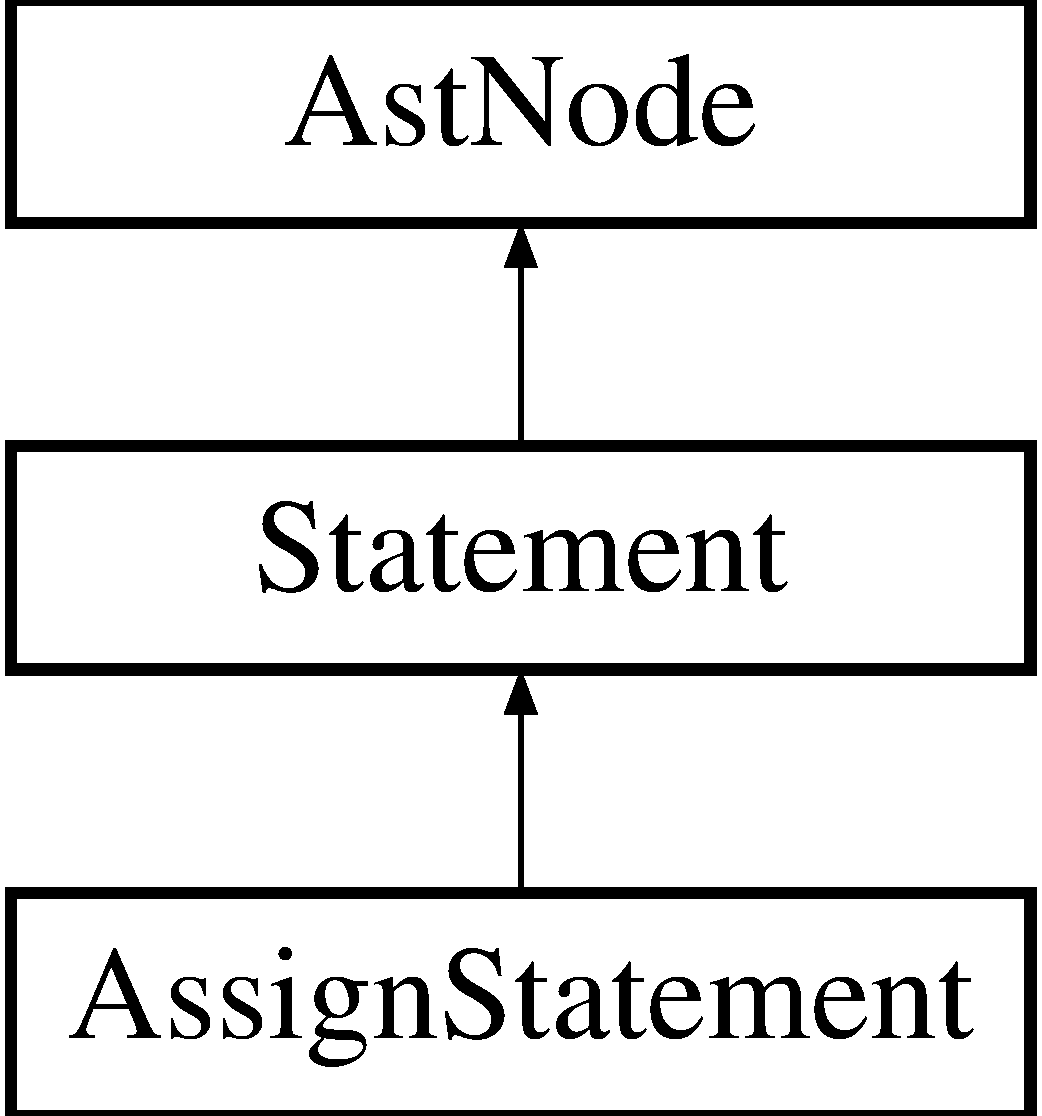
\includegraphics[height=3cm]{classAssignStatement}
\end{center}
\end{figure}
\subsection*{Public Member Functions}
\begin{DoxyCompactItemize}
\item 
\hyperlink{classAssignStatement_ad2cc7d861f58d9ebe7302aeca01975fb}{AssignStatement} (int lineNo, const char $\ast$lhsName, \hyperlink{classExpression}{Expression} $\ast$rhs)
\item 
\hyperlink{classAssignStatement_a54299cdd3f930c738a74bbff01200d9d}{AssignStatement} (int lineNo, const char $\ast$lhsName, \hyperlink{classExpression}{Expression} $\ast$idx, \hyperlink{classExpression}{Expression} $\ast$rhs)
\item 
const char $\ast$ \hyperlink{classAssignStatement_a9c6b348f0bcd4ca190414710ddeb085f}{getLHSName} ()
\item 
ENTRY $\ast$ \hyperlink{classAssignStatement_a4b640ab15accc35753ef8ae72c7b90fc}{getEntry} ()
\item 
void \hyperlink{classAssignStatement_a8a0b32169f7557553d24582f5b893ba2}{setEntry} (ENTRY $\ast$e)
\item 
\hyperlink{classExpression}{Expression} $\ast$ \hyperlink{classAssignStatement_a89a46624c82d07ce4b4f4819c2d7df81}{getIndex} ()
\item 
\hyperlink{classExpression}{Expression} $\ast$ \hyperlink{classAssignStatement_a488cf9857d458c808b97471a1a3789df}{getExpression} ()
\item 
void \hyperlink{classAssignStatement_a178a2773781301e16eebfd3d420dc98d}{accept} (\hyperlink{classAstVisitor}{AstVisitor} $\ast$aVisitor)
\end{DoxyCompactItemize}


\subsection{Detailed Description}
This class represents a TinyJava assignment statement. An assignment statement has:
\begin{DoxyItemize}
\item a left-\/hand side, which may be a simple name (a variable, parameter, or a class field), or an array reference with a subscript expression. A pointer to the symbol table ENTRY for the name may also be included.
\item a right-\/hand side, which is an expression.
\end{DoxyItemize}

ENTRY should be defined as a macro, and its value should be a class, which is the root of the symbol table entry hierarchy. Its default value is Entry. The macro should be defined at the beginning of the header file Ast.h. 

\subsection{Constructor \& Destructor Documentation}
\hypertarget{classAssignStatement_ad2cc7d861f58d9ebe7302aeca01975fb}{
\index{AssignStatement@{AssignStatement}!AssignStatement@{AssignStatement}}
\index{AssignStatement@{AssignStatement}!AssignStatement@{AssignStatement}}
\subsubsection[{AssignStatement}]{\setlength{\rightskip}{0pt plus 5cm}AssignStatement::AssignStatement (int {\em lineNo}, \/  const char $\ast$ {\em lhsName}, \/  {\bf Expression} $\ast$ {\em rhs})}}
\label{classAssignStatement_ad2cc7d861f58d9ebe7302aeca01975fb}
Create a assignment statement node, where the left-\/hand side is a simple variable, parameter, or a class field. 
\begin{DoxyParams}{Parameters}
\item[{\em lineNo}]is a source line number with the assignment statement \item[{\em lhsName}]is the name on the left-\/hand side of this assignment \item[{\em rhs}]is a pointer to an expression node representing the right-\/hand side expression \end{DoxyParams}

\begin{DoxyExceptions}{Exceptions}
\item[{\em \hyperlink{classAstException}{AstException}}]if the lhs or the rhs is NULL \end{DoxyExceptions}
\hypertarget{classAssignStatement_a54299cdd3f930c738a74bbff01200d9d}{
\index{AssignStatement@{AssignStatement}!AssignStatement@{AssignStatement}}
\index{AssignStatement@{AssignStatement}!AssignStatement@{AssignStatement}}
\subsubsection[{AssignStatement}]{\setlength{\rightskip}{0pt plus 5cm}AssignStatement::AssignStatement (int {\em lineNo}, \/  const char $\ast$ {\em lhsName}, \/  {\bf Expression} $\ast$ {\em idx}, \/  {\bf Expression} $\ast$ {\em rhs})}}
\label{classAssignStatement_a54299cdd3f930c738a74bbff01200d9d}
Create a assignment statement node, where the left-\/hand side is a simple variable, parameter, or a class field. 
\begin{DoxyParams}{Parameters}
\item[{\em lineNo}]is a source line number. \item[{\em lhsName}]is the name on the left-\/hand side of this assignment. \item[{\em idx}]is a pointer to an expression node representing the index (subscript) expression. \item[{\em rhs}]is a pointer to an expression node representing the right-\/hand side expression. \end{DoxyParams}

\begin{DoxyExceptions}{Exceptions}
\item[{\em \hyperlink{classAstException}{AstException}}]if the lhs or the rhs is NULL \end{DoxyExceptions}


\subsection{Member Function Documentation}
\hypertarget{classAssignStatement_a178a2773781301e16eebfd3d420dc98d}{
\index{AssignStatement@{AssignStatement}!accept@{accept}}
\index{accept@{accept}!AssignStatement@{AssignStatement}}
\subsubsection[{accept}]{\setlength{\rightskip}{0pt plus 5cm}void AssignStatement::accept ({\bf AstVisitor} $\ast$ {\em aVisitor})\hspace{0.3cm}{\ttfamily  \mbox{[}inline, virtual\mbox{]}}}}
\label{classAssignStatement_a178a2773781301e16eebfd3d420dc98d}
Accept a visitor to this node. 
\begin{DoxyParams}{Parameters}
\item[{\em aVisitor}]is a visitor object of type \hyperlink{classAstVisitor}{AstVisitor}. \end{DoxyParams}


Implements \hyperlink{classAstNode_a67b2d6ce1262da2954fb4db255759fb3}{AstNode}.\hypertarget{classAssignStatement_a4b640ab15accc35753ef8ae72c7b90fc}{
\index{AssignStatement@{AssignStatement}!getEntry@{getEntry}}
\index{getEntry@{getEntry}!AssignStatement@{AssignStatement}}
\subsubsection[{getEntry}]{\setlength{\rightskip}{0pt plus 5cm}ENTRY$\ast$ AssignStatement::getEntry ()\hspace{0.3cm}{\ttfamily  \mbox{[}inline\mbox{]}}}}
\label{classAssignStatement_a4b640ab15accc35753ef8ae72c7b90fc}
Return the symbol table entry representing the left-\/hand side of this assignment. \begin{DoxyReturn}{Returns}
ENTRY pointer to the symbol table. 
\end{DoxyReturn}
\hypertarget{classAssignStatement_a488cf9857d458c808b97471a1a3789df}{
\index{AssignStatement@{AssignStatement}!getExpression@{getExpression}}
\index{getExpression@{getExpression}!AssignStatement@{AssignStatement}}
\subsubsection[{getExpression}]{\setlength{\rightskip}{0pt plus 5cm}{\bf Expression}$\ast$ AssignStatement::getExpression ()\hspace{0.3cm}{\ttfamily  \mbox{[}inline\mbox{]}}}}
\label{classAssignStatement_a488cf9857d458c808b97471a1a3789df}
Return the expression pointer representing the right-\/hand side of this assignment. \begin{DoxyReturn}{Returns}
\hyperlink{classExpression}{Expression} pointer representing the right-\/hand side expression. 
\end{DoxyReturn}
\hypertarget{classAssignStatement_a89a46624c82d07ce4b4f4819c2d7df81}{
\index{AssignStatement@{AssignStatement}!getIndex@{getIndex}}
\index{getIndex@{getIndex}!AssignStatement@{AssignStatement}}
\subsubsection[{getIndex}]{\setlength{\rightskip}{0pt plus 5cm}{\bf Expression}$\ast$ AssignStatement::getIndex ()\hspace{0.3cm}{\ttfamily  \mbox{[}inline\mbox{]}}}}
\label{classAssignStatement_a89a46624c82d07ce4b4f4819c2d7df81}
Return the index expression, if the left hand side is an array element.

\begin{DoxyReturn}{Returns}
\hyperlink{classExpression}{Expression} pointer representing the array index (subscript). 
\end{DoxyReturn}
\hypertarget{classAssignStatement_a9c6b348f0bcd4ca190414710ddeb085f}{
\index{AssignStatement@{AssignStatement}!getLHSName@{getLHSName}}
\index{getLHSName@{getLHSName}!AssignStatement@{AssignStatement}}
\subsubsection[{getLHSName}]{\setlength{\rightskip}{0pt plus 5cm}const char$\ast$ AssignStatement::getLHSName ()\hspace{0.3cm}{\ttfamily  \mbox{[}inline\mbox{]}}}}
\label{classAssignStatement_a9c6b348f0bcd4ca190414710ddeb085f}
Return the identifier (variable, field, or parameter) on the left hand side of this assignment statement. \begin{DoxyReturn}{Returns}
const char $\ast$ pointer to the left-\/hand side identifier. 
\end{DoxyReturn}
\hypertarget{classAssignStatement_a8a0b32169f7557553d24582f5b893ba2}{
\index{AssignStatement@{AssignStatement}!setEntry@{setEntry}}
\index{setEntry@{setEntry}!AssignStatement@{AssignStatement}}
\subsubsection[{setEntry}]{\setlength{\rightskip}{0pt plus 5cm}void AssignStatement::setEntry (ENTRY $\ast$ {\em e})\hspace{0.3cm}{\ttfamily  \mbox{[}inline\mbox{]}}}}
\label{classAssignStatement_a8a0b32169f7557553d24582f5b893ba2}
Set the symbol table entry representing the left-\/hand side of this assignment.


\begin{DoxyParams}{Parameters}
\item[{\em e}]is the new pointer to the symbol table. \end{DoxyParams}


The documentation for this class was generated from the following files:\begin{DoxyCompactItemize}
\item 
AssignStmt.h\item 
AssignStmt.cpp\end{DoxyCompactItemize}

\hypertarget{classAstException}{
\section{AstException Class Reference}
\label{classAstException}\index{AstException@{AstException}}
}


This class represents an exception that may occur within the Abstract Syntax Tree Library for TinyJava.  


{\ttfamily \#include $<$AstException.h$>$}\subsection*{Public Member Functions}
\begin{DoxyCompactItemize}
\item 
\hyperlink{classAstException_aff6bd0191954f4c9d5bc2c1608d3e94e}{AstException} (const std::string \&msg)
\end{DoxyCompactItemize}


\subsection{Detailed Description}
This class represents an exception that may occur within the Abstract Syntax Tree Library for TinyJava. An \hyperlink{classAstException}{AstException} includes a message indicating the cause for the exception. 

\subsection{Constructor \& Destructor Documentation}
\hypertarget{classAstException_aff6bd0191954f4c9d5bc2c1608d3e94e}{
\index{AstException@{AstException}!AstException@{AstException}}
\index{AstException@{AstException}!AstException@{AstException}}
\subsubsection[{AstException}]{\setlength{\rightskip}{0pt plus 5cm}AstException::AstException (const std::string \& {\em msg})\hspace{0.3cm}{\ttfamily  \mbox{[}inline\mbox{]}}}}
\label{classAstException_aff6bd0191954f4c9d5bc2c1608d3e94e}
Construct an \hyperlink{classAstException}{AstException} exception object indicating a problem within an Abstract Syntax Tree.


\begin{DoxyParams}{Parameters}
\item[{\em msg}]a message describing the error. \end{DoxyParams}


The documentation for this class was generated from the following file:\begin{DoxyCompactItemize}
\item 
AstException.h\end{DoxyCompactItemize}

\hypertarget{classAstNode}{
\section{AstNode Class Reference}
\label{classAstNode}\index{AstNode@{AstNode}}
}


This is the root of the Abstract Syntax Tree class hierarchy.  


{\ttfamily \#include $<$AstNode.h$>$}Inheritance diagram for AstNode::\begin{figure}[H]
\begin{center}
\leavevmode
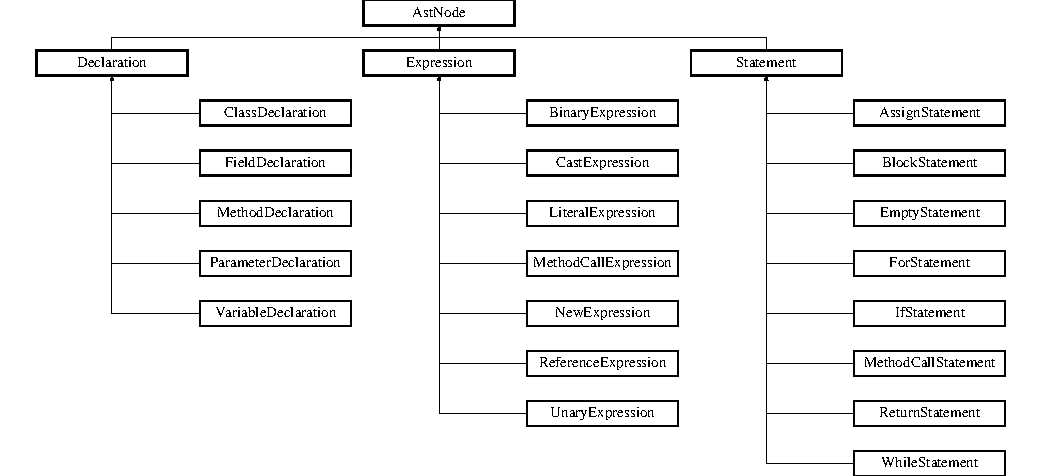
\includegraphics[height=6.39269cm]{classAstNode}
\end{center}
\end{figure}
\subsection*{Public Types}
\begin{DoxyCompactItemize}
\item 
enum \hyperlink{classAstNode_a365f519b5e9e517edc83566bd1cfe950}{AstNodeKind} \{ \par
\hyperlink{classAstNode_a365f519b5e9e517edc83566bd1cfe950a74f05149a25fe61dabeb25520382c1c2}{DCLASS}, 
\hyperlink{classAstNode_a365f519b5e9e517edc83566bd1cfe950af58ad2e4831b8c3c7789a3c4054642c5}{DFIELD}, 
\hyperlink{classAstNode_a365f519b5e9e517edc83566bd1cfe950ad3b8425047b32cc74fa3688c2da95761}{DMETHOD}, 
\hyperlink{classAstNode_a365f519b5e9e517edc83566bd1cfe950a1dd054e6f23331982e648d40a3a010f5}{DPARAMETER}, 
\par
\hyperlink{classAstNode_a365f519b5e9e517edc83566bd1cfe950a63ec96e21ca1021019b7e5d2f11e71b1}{DVARIABLE}, 
\hyperlink{classAstNode_a365f519b5e9e517edc83566bd1cfe950a36765da53ef4678d5e619ffe0e85307c}{ELITERAL}, 
\hyperlink{classAstNode_a365f519b5e9e517edc83566bd1cfe950a60af566d801917b1682de26a9e0004fd}{ENAME}, 
\hyperlink{classAstNode_a365f519b5e9e517edc83566bd1cfe950aab4b8cee1550e71c04537cce17c71edc}{ENEW}, 
\par
\hyperlink{classAstNode_a365f519b5e9e517edc83566bd1cfe950a4697428e167fee2f70f010c36dd3e9c8}{EUNARY}, 
\hyperlink{classAstNode_a365f519b5e9e517edc83566bd1cfe950a58ca86e25c2f6c444bf339818c1a9239}{EBINARY}, 
\hyperlink{classAstNode_a365f519b5e9e517edc83566bd1cfe950a1daa1362aa004cdefe437681ec66e299}{ECAST}, 
\hyperlink{classAstNode_a365f519b5e9e517edc83566bd1cfe950a3f693d520f9042b99bc39c5e11538812}{EMCALL}, 
\par
\hyperlink{classAstNode_a365f519b5e9e517edc83566bd1cfe950a07ad9af3faed1cd28726abe1ce7f2bdb}{SASSIGN}, 
\hyperlink{classAstNode_a365f519b5e9e517edc83566bd1cfe950ab5481ab4de7d88b5004055a0c7fb8629}{SWHILE}, 
\hyperlink{classAstNode_a365f519b5e9e517edc83566bd1cfe950a8e42e06272e07bffadee68c4d393ddbe}{SFOR}, 
\hyperlink{classAstNode_a365f519b5e9e517edc83566bd1cfe950a927858fb9744799e4e35e9ba9c577047}{SIF}, 
\par
\hyperlink{classAstNode_a365f519b5e9e517edc83566bd1cfe950aa831a911ca3a2eff7c1027846d133113}{SRETURN}, 
\hyperlink{classAstNode_a365f519b5e9e517edc83566bd1cfe950af7cb46f572219dca20fb4d0ad7280ad6}{SBLOCK}, 
\hyperlink{classAstNode_a365f519b5e9e517edc83566bd1cfe950a5d5130e3c308a4e74a2b77ebd2766052}{SMCALL}, 
\hyperlink{classAstNode_a365f519b5e9e517edc83566bd1cfe950a795546958814b99a16d59743f029eb55}{SEMPTY}
 \}
\end{DoxyCompactItemize}
\subsection*{Public Member Functions}
\begin{DoxyCompactItemize}
\item 
\hyperlink{classAstNode_a365f519b5e9e517edc83566bd1cfe950}{AstNodeKind} \hyperlink{classAstNode_ac18055137cc3544e330c42f0c41acf86}{getKind} ()
\item 
void \hyperlink{classAstNode_a1d7bf9b1d9cd668d155ddd86d22bc727}{setKind} (\hyperlink{classAstNode_a365f519b5e9e517edc83566bd1cfe950}{AstNodeKind} newKind)
\item 
int \hyperlink{classAstNode_a93ce204950529a50b86813904e03dfd7}{getLineNo} ()
\item 
void \hyperlink{classAstNode_abe694eb81a2d9042c571ecc2ca8d38e8}{setLineNo} (int lno)
\item 
virtual void \hyperlink{classAstNode_a67b2d6ce1262da2954fb4db255759fb3}{accept} (\hyperlink{classAstVisitor}{AstVisitor} $\ast$aVisitor)=0
\end{DoxyCompactItemize}
\subsection*{Static Public Member Functions}
\begin{DoxyCompactItemize}
\item 
static const char $\ast$ \hyperlink{classAstNode_a6b77773e4a27d8ca40bc1fce09d4764e}{type2string} (int tp)
\item 
static const char $\ast$ \hyperlink{classAstNode_abb3df00672c92269af102f415b9acf62}{operator2string} (int op)
\item 
static const char $\ast$ \hyperlink{classAstNode_a9579a36e66ca9449b8aac87f0bf8f832}{kind2string} (\hyperlink{classAstNode_a365f519b5e9e517edc83566bd1cfe950}{AstNodeKind} kind)
\end{DoxyCompactItemize}
\subsection*{Static Public Attributes}
\begin{DoxyCompactItemize}
\item 
static const int \hyperlink{classAstNode_ac664e0864b9c856e947d5fde632eb5e7}{TVOID} = 0
\item 
static const int \hyperlink{classAstNode_a8568313f5d280773a446280c94d382f8}{TINT} = 1
\item 
static const int \hyperlink{classAstNode_abf470f775bd7a7bfc2c0610716054339}{TFLOAT} = 2
\item 
static const int \hyperlink{classAstNode_a71904f4c33eff3bb3a37fadda88f12c9}{TBOOL} = 3
\item 
static const int \hyperlink{classAstNode_a2245a2aec841592ecddf8f9497306a4b}{TSTRING} = 4
\item 
static const int \hyperlink{classAstNode_a7233043e1a9d95c3120a62ac66c89608}{TINTA} = 5
\item 
static const int \hyperlink{classAstNode_a9d01a6ac8a4a7a5b2d4a3ec8a7e93fa7}{TFLOATA} = 6
\item 
static const int \hyperlink{classAstNode_ae3a9310b89b8c86afe245cf88ab1369a}{TSTRINGA} = 7
\item 
static const int \hyperlink{classAstNode_ad84a595b7727d93d325664d5bf89c766}{TREF} = 8
\item 
static const int \hyperlink{classAstNode_af908b13b6954116a438f86ce595d5bfe}{ADDOP} = 0
\item 
static const int \hyperlink{classAstNode_a8d62c361a16d84b762172fac68650561}{SUBOP} = 1
\item 
static const int \hyperlink{classAstNode_af1564bffc1a770122ea56654f4439531}{MULOP} = 2
\item 
static const int \hyperlink{classAstNode_a3972892cd58f1c70c84366804bdfd371}{DIVOP} = 3
\item 
static const int \hyperlink{classAstNode_a9cb6a842a496aed85756aa779789ce77}{EQOP} = 4
\item 
static const int \hyperlink{classAstNode_a3347eacf3e38675c075a7ce1c4cb6e29}{NEOP} = 5
\item 
static const int \hyperlink{classAstNode_a1ddf9dbcce4b80d311e7080b8262b65b}{LTOP} = 6
\item 
static const int \hyperlink{classAstNode_a3103a273c9da38b092334c757ee19ace}{GTOP} = 7
\item 
static const int \hyperlink{classAstNode_ac62da8b0313271a74293826f586dd6ea}{LEOP} = 8
\item 
static const int \hyperlink{classAstNode_aeb92e9f6e1407ff0c945f220b3da9820}{GEOP} = 9
\item 
static const int \hyperlink{classAstNode_abf9092d925819312d2547c414b493c4f}{INCOP} = 10
\item 
static const int \hyperlink{classAstNode_a0a48e47b23689fb51c059cb48a007adc}{DECOP} = 11
\end{DoxyCompactItemize}


\subsection{Detailed Description}
This is the root of the Abstract Syntax Tree class hierarchy. An \hyperlink{classAstNode}{AstNode} object represents an Abstract Syntax Tree (AST) Node. The \hyperlink{classAstNode}{AstNode} class hierarchy is subdivided into:
\begin{DoxyItemize}
\item declarations (subclasses of \hyperlink{classDeclaration}{Declaration}),
\item expressions (subclasses of \hyperlink{classExpression}{Expression}), and
\item statements (subclasses of \hyperlink{classStatement}{Statement}).
\end{DoxyItemize}

There are several types (kinds) of concrete AST nodes. More specifically, a node can be:
\begin{DoxyItemize}
\item a declaration node (a subclass of \hyperlink{classDeclaration}{Declaration}) of type: DCLASS, DMETHOD, DFIELD, DPARAMETER, DVARIABLE
\item an expression node (a subclass of \hyperlink{classExpression}{Expression}) of type: ELITERAL, ENAME, EUNARY, EBINARY, ECAST, EMCALL,
\item a statement node (a subclass of \hyperlink{classStatement}{Statement}) of type: SASSIGN, SWHILE, SIF, SRETURN, SBLOCK, SMCALL, SEMPTY 
\end{DoxyItemize}

\subsection{Member Enumeration Documentation}
\hypertarget{classAstNode_a365f519b5e9e517edc83566bd1cfe950}{
\index{AstNode@{AstNode}!AstNodeKind@{AstNodeKind}}
\index{AstNodeKind@{AstNodeKind}!AstNode@{AstNode}}
\subsubsection[{AstNodeKind}]{\setlength{\rightskip}{0pt plus 5cm}enum {\bf AstNode::AstNodeKind}}}
\label{classAstNode_a365f519b5e9e517edc83566bd1cfe950}
This enumeration type elements are used to represent the kinds of Abstract Syntax Tree nodes. \begin{Desc}
\item[Enumerator: ]\par
\begin{description}
\index{DCLASS@{DCLASS}!AstNode@{AstNode}}\index{AstNode@{AstNode}!DCLASS@{DCLASS}}\item[{\em 
\hypertarget{classAstNode_a365f519b5e9e517edc83566bd1cfe950a74f05149a25fe61dabeb25520382c1c2}{
DCLASS}
\label{classAstNode_a365f519b5e9e517edc83566bd1cfe950a74f05149a25fe61dabeb25520382c1c2}
}]a class declaration node \index{DFIELD@{DFIELD}!AstNode@{AstNode}}\index{AstNode@{AstNode}!DFIELD@{DFIELD}}\item[{\em 
\hypertarget{classAstNode_a365f519b5e9e517edc83566bd1cfe950af58ad2e4831b8c3c7789a3c4054642c5}{
DFIELD}
\label{classAstNode_a365f519b5e9e517edc83566bd1cfe950af58ad2e4831b8c3c7789a3c4054642c5}
}]a field declaration node \index{DMETHOD@{DMETHOD}!AstNode@{AstNode}}\index{AstNode@{AstNode}!DMETHOD@{DMETHOD}}\item[{\em 
\hypertarget{classAstNode_a365f519b5e9e517edc83566bd1cfe950ad3b8425047b32cc74fa3688c2da95761}{
DMETHOD}
\label{classAstNode_a365f519b5e9e517edc83566bd1cfe950ad3b8425047b32cc74fa3688c2da95761}
}]a method declaration node \index{DPARAMETER@{DPARAMETER}!AstNode@{AstNode}}\index{AstNode@{AstNode}!DPARAMETER@{DPARAMETER}}\item[{\em 
\hypertarget{classAstNode_a365f519b5e9e517edc83566bd1cfe950a1dd054e6f23331982e648d40a3a010f5}{
DPARAMETER}
\label{classAstNode_a365f519b5e9e517edc83566bd1cfe950a1dd054e6f23331982e648d40a3a010f5}
}]a parameter declaration node \index{DVARIABLE@{DVARIABLE}!AstNode@{AstNode}}\index{AstNode@{AstNode}!DVARIABLE@{DVARIABLE}}\item[{\em 
\hypertarget{classAstNode_a365f519b5e9e517edc83566bd1cfe950a63ec96e21ca1021019b7e5d2f11e71b1}{
DVARIABLE}
\label{classAstNode_a365f519b5e9e517edc83566bd1cfe950a63ec96e21ca1021019b7e5d2f11e71b1}
}]a variabale declaration node \index{ELITERAL@{ELITERAL}!AstNode@{AstNode}}\index{AstNode@{AstNode}!ELITERAL@{ELITERAL}}\item[{\em 
\hypertarget{classAstNode_a365f519b5e9e517edc83566bd1cfe950a36765da53ef4678d5e619ffe0e85307c}{
ELITERAL}
\label{classAstNode_a365f519b5e9e517edc83566bd1cfe950a36765da53ef4678d5e619ffe0e85307c}
}]a literal expression node \index{ENAME@{ENAME}!AstNode@{AstNode}}\index{AstNode@{AstNode}!ENAME@{ENAME}}\item[{\em 
\hypertarget{classAstNode_a365f519b5e9e517edc83566bd1cfe950a60af566d801917b1682de26a9e0004fd}{
ENAME}
\label{classAstNode_a365f519b5e9e517edc83566bd1cfe950a60af566d801917b1682de26a9e0004fd}
}]a name reference expression node (may be a vriable, parameter, or a field) \index{ENEW@{ENEW}!AstNode@{AstNode}}\index{AstNode@{AstNode}!ENEW@{ENEW}}\item[{\em 
\hypertarget{classAstNode_a365f519b5e9e517edc83566bd1cfe950aab4b8cee1550e71c04537cce17c71edc}{
ENEW}
\label{classAstNode_a365f519b5e9e517edc83566bd1cfe950aab4b8cee1550e71c04537cce17c71edc}
}]a NEW expression node (just for array construction) \index{EUNARY@{EUNARY}!AstNode@{AstNode}}\index{AstNode@{AstNode}!EUNARY@{EUNARY}}\item[{\em 
\hypertarget{classAstNode_a365f519b5e9e517edc83566bd1cfe950a4697428e167fee2f70f010c36dd3e9c8}{
EUNARY}
\label{classAstNode_a365f519b5e9e517edc83566bd1cfe950a4697428e167fee2f70f010c36dd3e9c8}
}]a unary expression node (may be prefix or postfix) \index{EBINARY@{EBINARY}!AstNode@{AstNode}}\index{AstNode@{AstNode}!EBINARY@{EBINARY}}\item[{\em 
\hypertarget{classAstNode_a365f519b5e9e517edc83566bd1cfe950a58ca86e25c2f6c444bf339818c1a9239}{
EBINARY}
\label{classAstNode_a365f519b5e9e517edc83566bd1cfe950a58ca86e25c2f6c444bf339818c1a9239}
}]a binary expression node \index{ECAST@{ECAST}!AstNode@{AstNode}}\index{AstNode@{AstNode}!ECAST@{ECAST}}\item[{\em 
\hypertarget{classAstNode_a365f519b5e9e517edc83566bd1cfe950a1daa1362aa004cdefe437681ec66e299}{
ECAST}
\label{classAstNode_a365f519b5e9e517edc83566bd1cfe950a1daa1362aa004cdefe437681ec66e299}
}]a type cast expression node \index{EMCALL@{EMCALL}!AstNode@{AstNode}}\index{AstNode@{AstNode}!EMCALL@{EMCALL}}\item[{\em 
\hypertarget{classAstNode_a365f519b5e9e517edc83566bd1cfe950a3f693d520f9042b99bc39c5e11538812}{
EMCALL}
\label{classAstNode_a365f519b5e9e517edc83566bd1cfe950a3f693d520f9042b99bc39c5e11538812}
}]a method call expression node \index{SASSIGN@{SASSIGN}!AstNode@{AstNode}}\index{AstNode@{AstNode}!SASSIGN@{SASSIGN}}\item[{\em 
\hypertarget{classAstNode_a365f519b5e9e517edc83566bd1cfe950a07ad9af3faed1cd28726abe1ce7f2bdb}{
SASSIGN}
\label{classAstNode_a365f519b5e9e517edc83566bd1cfe950a07ad9af3faed1cd28726abe1ce7f2bdb}
}]an assignment statement node \index{SWHILE@{SWHILE}!AstNode@{AstNode}}\index{AstNode@{AstNode}!SWHILE@{SWHILE}}\item[{\em 
\hypertarget{classAstNode_a365f519b5e9e517edc83566bd1cfe950ab5481ab4de7d88b5004055a0c7fb8629}{
SWHILE}
\label{classAstNode_a365f519b5e9e517edc83566bd1cfe950ab5481ab4de7d88b5004055a0c7fb8629}
}]a WHILE statement node \index{SFOR@{SFOR}!AstNode@{AstNode}}\index{AstNode@{AstNode}!SFOR@{SFOR}}\item[{\em 
\hypertarget{classAstNode_a365f519b5e9e517edc83566bd1cfe950a8e42e06272e07bffadee68c4d393ddbe}{
SFOR}
\label{classAstNode_a365f519b5e9e517edc83566bd1cfe950a8e42e06272e07bffadee68c4d393ddbe}
}]a FOR statement node \index{SIF@{SIF}!AstNode@{AstNode}}\index{AstNode@{AstNode}!SIF@{SIF}}\item[{\em 
\hypertarget{classAstNode_a365f519b5e9e517edc83566bd1cfe950a927858fb9744799e4e35e9ba9c577047}{
SIF}
\label{classAstNode_a365f519b5e9e517edc83566bd1cfe950a927858fb9744799e4e35e9ba9c577047}
}]an IF statement node \index{SRETURN@{SRETURN}!AstNode@{AstNode}}\index{AstNode@{AstNode}!SRETURN@{SRETURN}}\item[{\em 
\hypertarget{classAstNode_a365f519b5e9e517edc83566bd1cfe950aa831a911ca3a2eff7c1027846d133113}{
SRETURN}
\label{classAstNode_a365f519b5e9e517edc83566bd1cfe950aa831a911ca3a2eff7c1027846d133113}
}]a return statement node \index{SBLOCK@{SBLOCK}!AstNode@{AstNode}}\index{AstNode@{AstNode}!SBLOCK@{SBLOCK}}\item[{\em 
\hypertarget{classAstNode_a365f519b5e9e517edc83566bd1cfe950af7cb46f572219dca20fb4d0ad7280ad6}{
SBLOCK}
\label{classAstNode_a365f519b5e9e517edc83566bd1cfe950af7cb46f572219dca20fb4d0ad7280ad6}
}]a block statement node \index{SMCALL@{SMCALL}!AstNode@{AstNode}}\index{AstNode@{AstNode}!SMCALL@{SMCALL}}\item[{\em 
\hypertarget{classAstNode_a365f519b5e9e517edc83566bd1cfe950a5d5130e3c308a4e74a2b77ebd2766052}{
SMCALL}
\label{classAstNode_a365f519b5e9e517edc83566bd1cfe950a5d5130e3c308a4e74a2b77ebd2766052}
}]a method call statement (a wrapper for a method call expression node) \index{SEMPTY@{SEMPTY}!AstNode@{AstNode}}\index{AstNode@{AstNode}!SEMPTY@{SEMPTY}}\item[{\em 
\hypertarget{classAstNode_a365f519b5e9e517edc83566bd1cfe950a795546958814b99a16d59743f029eb55}{
SEMPTY}
\label{classAstNode_a365f519b5e9e517edc83566bd1cfe950a795546958814b99a16d59743f029eb55}
}]an empty statement node \end{description}
\end{Desc}



\subsection{Member Function Documentation}
\hypertarget{classAstNode_a67b2d6ce1262da2954fb4db255759fb3}{
\index{AstNode@{AstNode}!accept@{accept}}
\index{accept@{accept}!AstNode@{AstNode}}
\subsubsection[{accept}]{\setlength{\rightskip}{0pt plus 5cm}virtual void AstNode::accept ({\bf AstVisitor} $\ast$ {\em aVisitor})\hspace{0.3cm}{\ttfamily  \mbox{[}pure virtual\mbox{]}}}}
\label{classAstNode_a67b2d6ce1262da2954fb4db255759fb3}
Accept a visitor to this node. 
\begin{DoxyParams}{Parameters}
\item[{\em aVisitor}]is a visitor object of type \hyperlink{classAstVisitor}{AstVisitor}. \end{DoxyParams}


Implemented in \hyperlink{classAssignStatement_a178a2773781301e16eebfd3d420dc98d}{AssignStatement}, \hyperlink{classBinaryExpression_a2af7e73b6a90c216ef00b6297ce83da5}{BinaryExpression}, \hyperlink{classBlockStatement_a20df05e7536e375226639b483e8c4732}{BlockStatement}, \hyperlink{classCastExpression_af98e34f83dce5fec6d21f4baf4679dea}{CastExpression}, \hyperlink{classClassDeclaration_abb1e806c4c54cfecbc685b5c8a072eae}{ClassDeclaration}, \hyperlink{classEmptyStatement_a54138a042d8de2fecf90448a0048757b}{EmptyStatement}, \hyperlink{classFieldDeclaration_a60ce09d75a5864803ca3b24530267af1}{FieldDeclaration}, \hyperlink{classForStatement_a8d31a952806bc123a2f6227d4aa17f2f}{ForStatement}, \hyperlink{classIfStatement_ab4c2cd2f1c924951d782493281d15249}{IfStatement}, \hyperlink{classLiteralExpression_a02054e805df96a9d75ea64acc35d15a7}{LiteralExpression}, \hyperlink{classMethodCallExpression_a306fe23511d0d35c003a6256816ccea6}{MethodCallExpression}, \hyperlink{classMethodCallStatement_a4bbae8f172868a47ba651f436087e16f}{MethodCallStatement}, \hyperlink{classMethodDeclaration_af4989b6bfa1fdc87be33f4315aa54a7e}{MethodDeclaration}, \hyperlink{classNewExpression_a4b5178e78150432ac58a08197204fa27}{NewExpression}, \hyperlink{classParameterDeclaration_a7e9679286d169930445a159abd5e42ad}{ParameterDeclaration}, \hyperlink{classReferenceExpression_a5235ddeb368f790fd69b73dc1fe5a80e}{ReferenceExpression}, \hyperlink{classReturnStatement_a491cb39772b9054be31d27dbc0d72d0f}{ReturnStatement}, \hyperlink{classUnaryExpression_a555e53bb0a187856275b8d2c885b75d0}{UnaryExpression}, \hyperlink{classVariableDeclaration_af8e0086b00a9bc45f2aff7bf91d8f17d}{VariableDeclaration}, and \hyperlink{classWhileStatement_aeb7e6e61053a3e8a7b82a54c4eb8bf0d}{WhileStatement}.\hypertarget{classAstNode_ac18055137cc3544e330c42f0c41acf86}{
\index{AstNode@{AstNode}!getKind@{getKind}}
\index{getKind@{getKind}!AstNode@{AstNode}}
\subsubsection[{getKind}]{\setlength{\rightskip}{0pt plus 5cm}{\bf AstNodeKind} AstNode::getKind ()\hspace{0.3cm}{\ttfamily  \mbox{[}inline\mbox{]}}}}
\label{classAstNode_ac18055137cc3544e330c42f0c41acf86}
Return the type (kind) of this node. \begin{DoxyReturn}{Returns}
the node kind (of type AstNodeKind) 
\end{DoxyReturn}
\hypertarget{classAstNode_a93ce204950529a50b86813904e03dfd7}{
\index{AstNode@{AstNode}!getLineNo@{getLineNo}}
\index{getLineNo@{getLineNo}!AstNode@{AstNode}}
\subsubsection[{getLineNo}]{\setlength{\rightskip}{0pt plus 5cm}int AstNode::getLineNo ()\hspace{0.3cm}{\ttfamily  \mbox{[}inline\mbox{]}}}}
\label{classAstNode_a93ce204950529a50b86813904e03dfd7}
Return the source line number of this node. \begin{DoxyReturn}{Returns}
the line number 
\end{DoxyReturn}
\hypertarget{classAstNode_a9579a36e66ca9449b8aac87f0bf8f832}{
\index{AstNode@{AstNode}!kind2string@{kind2string}}
\index{kind2string@{kind2string}!AstNode@{AstNode}}
\subsubsection[{kind2string}]{\setlength{\rightskip}{0pt plus 5cm}const char $\ast$ AstNode::kind2string ({\bf AstNode::AstNodeKind} {\em kind})\hspace{0.3cm}{\ttfamily  \mbox{[}static\mbox{]}}}}
\label{classAstNode_a9579a36e66ca9449b8aac87f0bf8f832}
Return a string representation of an \hyperlink{classAstNode}{AstNode} kind


\begin{DoxyParams}{Parameters}
\item[{\em kind}]an AstNodeKind value, as defined in the \hyperlink{classAstNode}{AstNode} class\end{DoxyParams}
\begin{DoxyReturn}{Returns}
a string representation of the \hyperlink{classAstNode}{AstNode} kind 
\end{DoxyReturn}
\hypertarget{classAstNode_abb3df00672c92269af102f415b9acf62}{
\index{AstNode@{AstNode}!operator2string@{operator2string}}
\index{operator2string@{operator2string}!AstNode@{AstNode}}
\subsubsection[{operator2string}]{\setlength{\rightskip}{0pt plus 5cm}const char $\ast$ AstNode::operator2string (int {\em op})\hspace{0.3cm}{\ttfamily  \mbox{[}static\mbox{]}}}}
\label{classAstNode_abb3df00672c92269af102f415b9acf62}
Return a string representation of a TinyJava operator


\begin{DoxyParams}{Parameters}
\item[{\em op}]an operator representation, as defined in the \hyperlink{classAstNode}{AstNode} class\end{DoxyParams}
\begin{DoxyReturn}{Returns}
a string representation of the operator 
\end{DoxyReturn}
\hypertarget{classAstNode_a1d7bf9b1d9cd668d155ddd86d22bc727}{
\index{AstNode@{AstNode}!setKind@{setKind}}
\index{setKind@{setKind}!AstNode@{AstNode}}
\subsubsection[{setKind}]{\setlength{\rightskip}{0pt plus 5cm}void AstNode::setKind ({\bf AstNodeKind} {\em newKind})\hspace{0.3cm}{\ttfamily  \mbox{[}inline\mbox{]}}}}
\label{classAstNode_a1d7bf9b1d9cd668d155ddd86d22bc727}
Set the type (kind) of this node. 
\begin{DoxyParams}{Parameters}
\item[{\em newKind}]is a new node type (kind). \end{DoxyParams}
\hypertarget{classAstNode_abe694eb81a2d9042c571ecc2ca8d38e8}{
\index{AstNode@{AstNode}!setLineNo@{setLineNo}}
\index{setLineNo@{setLineNo}!AstNode@{AstNode}}
\subsubsection[{setLineNo}]{\setlength{\rightskip}{0pt plus 5cm}void AstNode::setLineNo (int {\em lno})\hspace{0.3cm}{\ttfamily  \mbox{[}inline\mbox{]}}}}
\label{classAstNode_abe694eb81a2d9042c571ecc2ca8d38e8}
Set the source line number for this node 
\begin{DoxyParams}{Parameters}
\item[{\em lno}]is a source code line number for this \hyperlink{classAstNode}{AstNode} (a positive integer). \end{DoxyParams}
\hypertarget{classAstNode_a6b77773e4a27d8ca40bc1fce09d4764e}{
\index{AstNode@{AstNode}!type2string@{type2string}}
\index{type2string@{type2string}!AstNode@{AstNode}}
\subsubsection[{type2string}]{\setlength{\rightskip}{0pt plus 5cm}const char $\ast$ AstNode::type2string (int {\em tp})\hspace{0.3cm}{\ttfamily  \mbox{[}static\mbox{]}}}}
\label{classAstNode_a6b77773e4a27d8ca40bc1fce09d4764e}
Return a string representation of a TinyJava type


\begin{DoxyParams}{Parameters}
\item[{\em tp}]a type representation, as defined in the \hyperlink{classAstNode}{AstNode} class\end{DoxyParams}
\begin{DoxyReturn}{Returns}
a string representation of the type 
\end{DoxyReturn}


\subsection{Member Data Documentation}
\hypertarget{classAstNode_af908b13b6954116a438f86ce595d5bfe}{
\index{AstNode@{AstNode}!ADDOP@{ADDOP}}
\index{ADDOP@{ADDOP}!AstNode@{AstNode}}
\subsubsection[{ADDOP}]{\setlength{\rightskip}{0pt plus 5cm}const int {\bf AstNode::ADDOP} = 0\hspace{0.3cm}{\ttfamily  \mbox{[}static\mbox{]}}}}
\label{classAstNode_af908b13b6954116a438f86ce595d5bfe}
These constants are used to represent the TinyJava operators. '+' operator representation (prefix or infix) \hypertarget{classAstNode_a0a48e47b23689fb51c059cb48a007adc}{
\index{AstNode@{AstNode}!DECOP@{DECOP}}
\index{DECOP@{DECOP}!AstNode@{AstNode}}
\subsubsection[{DECOP}]{\setlength{\rightskip}{0pt plus 5cm}const int {\bf AstNode::DECOP} = 11\hspace{0.3cm}{\ttfamily  \mbox{[}static\mbox{]}}}}
\label{classAstNode_a0a48e47b23689fb51c059cb48a007adc}
'-\/-\/' operator (postfix) \hypertarget{classAstNode_a3972892cd58f1c70c84366804bdfd371}{
\index{AstNode@{AstNode}!DIVOP@{DIVOP}}
\index{DIVOP@{DIVOP}!AstNode@{AstNode}}
\subsubsection[{DIVOP}]{\setlength{\rightskip}{0pt plus 5cm}const int {\bf AstNode::DIVOP} = 3\hspace{0.3cm}{\ttfamily  \mbox{[}static\mbox{]}}}}
\label{classAstNode_a3972892cd58f1c70c84366804bdfd371}
'$\ast$' operator \hypertarget{classAstNode_a9cb6a842a496aed85756aa779789ce77}{
\index{AstNode@{AstNode}!EQOP@{EQOP}}
\index{EQOP@{EQOP}!AstNode@{AstNode}}
\subsubsection[{EQOP}]{\setlength{\rightskip}{0pt plus 5cm}const int {\bf AstNode::EQOP} = 4\hspace{0.3cm}{\ttfamily  \mbox{[}static\mbox{]}}}}
\label{classAstNode_a9cb6a842a496aed85756aa779789ce77}
'==' operator \hypertarget{classAstNode_aeb92e9f6e1407ff0c945f220b3da9820}{
\index{AstNode@{AstNode}!GEOP@{GEOP}}
\index{GEOP@{GEOP}!AstNode@{AstNode}}
\subsubsection[{GEOP}]{\setlength{\rightskip}{0pt plus 5cm}const int {\bf AstNode::GEOP} = 9\hspace{0.3cm}{\ttfamily  \mbox{[}static\mbox{]}}}}
\label{classAstNode_aeb92e9f6e1407ff0c945f220b3da9820}
'$>$=$\ast$' operator \hypertarget{classAstNode_a3103a273c9da38b092334c757ee19ace}{
\index{AstNode@{AstNode}!GTOP@{GTOP}}
\index{GTOP@{GTOP}!AstNode@{AstNode}}
\subsubsection[{GTOP}]{\setlength{\rightskip}{0pt plus 5cm}const int {\bf AstNode::GTOP} = 7\hspace{0.3cm}{\ttfamily  \mbox{[}static\mbox{]}}}}
\label{classAstNode_a3103a273c9da38b092334c757ee19ace}
'$>$' operator \hypertarget{classAstNode_abf9092d925819312d2547c414b493c4f}{
\index{AstNode@{AstNode}!INCOP@{INCOP}}
\index{INCOP@{INCOP}!AstNode@{AstNode}}
\subsubsection[{INCOP}]{\setlength{\rightskip}{0pt plus 5cm}const int {\bf AstNode::INCOP} = 10\hspace{0.3cm}{\ttfamily  \mbox{[}static\mbox{]}}}}
\label{classAstNode_abf9092d925819312d2547c414b493c4f}
'++' operator (postfix) \hypertarget{classAstNode_ac62da8b0313271a74293826f586dd6ea}{
\index{AstNode@{AstNode}!LEOP@{LEOP}}
\index{LEOP@{LEOP}!AstNode@{AstNode}}
\subsubsection[{LEOP}]{\setlength{\rightskip}{0pt plus 5cm}const int {\bf AstNode::LEOP} = 8\hspace{0.3cm}{\ttfamily  \mbox{[}static\mbox{]}}}}
\label{classAstNode_ac62da8b0313271a74293826f586dd6ea}
'$<$=' operator \hypertarget{classAstNode_a1ddf9dbcce4b80d311e7080b8262b65b}{
\index{AstNode@{AstNode}!LTOP@{LTOP}}
\index{LTOP@{LTOP}!AstNode@{AstNode}}
\subsubsection[{LTOP}]{\setlength{\rightskip}{0pt plus 5cm}const int {\bf AstNode::LTOP} = 6\hspace{0.3cm}{\ttfamily  \mbox{[}static\mbox{]}}}}
\label{classAstNode_a1ddf9dbcce4b80d311e7080b8262b65b}
'$<$' operator \hypertarget{classAstNode_af1564bffc1a770122ea56654f4439531}{
\index{AstNode@{AstNode}!MULOP@{MULOP}}
\index{MULOP@{MULOP}!AstNode@{AstNode}}
\subsubsection[{MULOP}]{\setlength{\rightskip}{0pt plus 5cm}const int {\bf AstNode::MULOP} = 2\hspace{0.3cm}{\ttfamily  \mbox{[}static\mbox{]}}}}
\label{classAstNode_af1564bffc1a770122ea56654f4439531}
'$\ast$' operator \hypertarget{classAstNode_a3347eacf3e38675c075a7ce1c4cb6e29}{
\index{AstNode@{AstNode}!NEOP@{NEOP}}
\index{NEOP@{NEOP}!AstNode@{AstNode}}
\subsubsection[{NEOP}]{\setlength{\rightskip}{0pt plus 5cm}const int {\bf AstNode::NEOP} = 5\hspace{0.3cm}{\ttfamily  \mbox{[}static\mbox{]}}}}
\label{classAstNode_a3347eacf3e38675c075a7ce1c4cb6e29}
'!=' operator \hypertarget{classAstNode_a8d62c361a16d84b762172fac68650561}{
\index{AstNode@{AstNode}!SUBOP@{SUBOP}}
\index{SUBOP@{SUBOP}!AstNode@{AstNode}}
\subsubsection[{SUBOP}]{\setlength{\rightskip}{0pt plus 5cm}const int {\bf AstNode::SUBOP} = 1\hspace{0.3cm}{\ttfamily  \mbox{[}static\mbox{]}}}}
\label{classAstNode_a8d62c361a16d84b762172fac68650561}
'-\/' operator representation (prefix or infix) \hypertarget{classAstNode_a71904f4c33eff3bb3a37fadda88f12c9}{
\index{AstNode@{AstNode}!TBOOL@{TBOOL}}
\index{TBOOL@{TBOOL}!AstNode@{AstNode}}
\subsubsection[{TBOOL}]{\setlength{\rightskip}{0pt plus 5cm}const int {\bf AstNode::TBOOL} = 3\hspace{0.3cm}{\ttfamily  \mbox{[}static\mbox{]}}}}
\label{classAstNode_a71904f4c33eff3bb3a37fadda88f12c9}
boolean type representation \hypertarget{classAstNode_abf470f775bd7a7bfc2c0610716054339}{
\index{AstNode@{AstNode}!TFLOAT@{TFLOAT}}
\index{TFLOAT@{TFLOAT}!AstNode@{AstNode}}
\subsubsection[{TFLOAT}]{\setlength{\rightskip}{0pt plus 5cm}const int {\bf AstNode::TFLOAT} = 2\hspace{0.3cm}{\ttfamily  \mbox{[}static\mbox{]}}}}
\label{classAstNode_abf470f775bd7a7bfc2c0610716054339}
float type representation \hypertarget{classAstNode_a9d01a6ac8a4a7a5b2d4a3ec8a7e93fa7}{
\index{AstNode@{AstNode}!TFLOATA@{TFLOATA}}
\index{TFLOATA@{TFLOATA}!AstNode@{AstNode}}
\subsubsection[{TFLOATA}]{\setlength{\rightskip}{0pt plus 5cm}const int {\bf AstNode::TFLOATA} = 6\hspace{0.3cm}{\ttfamily  \mbox{[}static\mbox{]}}}}
\label{classAstNode_a9d01a6ac8a4a7a5b2d4a3ec8a7e93fa7}
float\mbox{[}\mbox{]} type representation \hypertarget{classAstNode_a8568313f5d280773a446280c94d382f8}{
\index{AstNode@{AstNode}!TINT@{TINT}}
\index{TINT@{TINT}!AstNode@{AstNode}}
\subsubsection[{TINT}]{\setlength{\rightskip}{0pt plus 5cm}const int {\bf AstNode::TINT} = 1\hspace{0.3cm}{\ttfamily  \mbox{[}static\mbox{]}}}}
\label{classAstNode_a8568313f5d280773a446280c94d382f8}
int type representation \hypertarget{classAstNode_a7233043e1a9d95c3120a62ac66c89608}{
\index{AstNode@{AstNode}!TINTA@{TINTA}}
\index{TINTA@{TINTA}!AstNode@{AstNode}}
\subsubsection[{TINTA}]{\setlength{\rightskip}{0pt plus 5cm}const int {\bf AstNode::TINTA} = 5\hspace{0.3cm}{\ttfamily  \mbox{[}static\mbox{]}}}}
\label{classAstNode_a7233043e1a9d95c3120a62ac66c89608}
int\mbox{[}\mbox{]} type representation \hypertarget{classAstNode_ad84a595b7727d93d325664d5bf89c766}{
\index{AstNode@{AstNode}!TREF@{TREF}}
\index{TREF@{TREF}!AstNode@{AstNode}}
\subsubsection[{TREF}]{\setlength{\rightskip}{0pt plus 5cm}const int {\bf AstNode::TREF} = 8\hspace{0.3cm}{\ttfamily  \mbox{[}static\mbox{]}}}}
\label{classAstNode_ad84a595b7727d93d325664d5bf89c766}
basic reference type representation (to be used for null expression type) \hypertarget{classAstNode_a2245a2aec841592ecddf8f9497306a4b}{
\index{AstNode@{AstNode}!TSTRING@{TSTRING}}
\index{TSTRING@{TSTRING}!AstNode@{AstNode}}
\subsubsection[{TSTRING}]{\setlength{\rightskip}{0pt plus 5cm}const int {\bf AstNode::TSTRING} = 4\hspace{0.3cm}{\ttfamily  \mbox{[}static\mbox{]}}}}
\label{classAstNode_a2245a2aec841592ecddf8f9497306a4b}
String type representation \hypertarget{classAstNode_ae3a9310b89b8c86afe245cf88ab1369a}{
\index{AstNode@{AstNode}!TSTRINGA@{TSTRINGA}}
\index{TSTRINGA@{TSTRINGA}!AstNode@{AstNode}}
\subsubsection[{TSTRINGA}]{\setlength{\rightskip}{0pt plus 5cm}const int {\bf AstNode::TSTRINGA} = 7\hspace{0.3cm}{\ttfamily  \mbox{[}static\mbox{]}}}}
\label{classAstNode_ae3a9310b89b8c86afe245cf88ab1369a}
String\mbox{[}\mbox{]} type representation \hypertarget{classAstNode_ac664e0864b9c856e947d5fde632eb5e7}{
\index{AstNode@{AstNode}!TVOID@{TVOID}}
\index{TVOID@{TVOID}!AstNode@{AstNode}}
\subsubsection[{TVOID}]{\setlength{\rightskip}{0pt plus 5cm}const int {\bf AstNode::TVOID} = 0\hspace{0.3cm}{\ttfamily  \mbox{[}static\mbox{]}}}}
\label{classAstNode_ac664e0864b9c856e947d5fde632eb5e7}
These constants are used to represent the TinyJava types. void type representation 

The documentation for this class was generated from the following files:\begin{DoxyCompactItemize}
\item 
AstNode.h\item 
AstNode.cpp\end{DoxyCompactItemize}

\hypertarget{classAstVisitor}{
\section{AstVisitor Class Reference}
\label{classAstVisitor}\index{AstVisitor@{AstVisitor}}
}


This is the parent of all Abstract Syntax Tree visitors; it is an abstract class.  


{\ttfamily \#include $<$AstVisitor.h$>$}\subsection*{Public Member Functions}
\begin{DoxyCompactItemize}
\item 
virtual void \hyperlink{classAstVisitor_ae922c774d8e8e3fbb9a81a229ef00ecb}{visit} (\hyperlink{classClassDeclaration}{ClassDeclaration} $\ast$aDeclNode)=0
\item 
virtual void \hyperlink{classAstVisitor_ab9d4c10a46ea5252fb90a76f347852af}{visit} (\hyperlink{classMethodDeclaration}{MethodDeclaration} $\ast$aDeclNode)=0
\item 
virtual void \hyperlink{classAstVisitor_a15ca20c155aa1b3c67c983dc9ecf10a7}{visit} (\hyperlink{classFieldDeclaration}{FieldDeclaration} $\ast$aDeclNode)=0
\item 
virtual void \hyperlink{classAstVisitor_a55c262f146345bdeb890ba032e08650a}{visit} (\hyperlink{classParameterDeclaration}{ParameterDeclaration} $\ast$aDeclNode)=0
\item 
virtual void \hyperlink{classAstVisitor_a7b11f0796ae296e3edc720de75a496c3}{visit} (\hyperlink{classVariableDeclaration}{VariableDeclaration} $\ast$aDeclNode)=0
\item 
virtual void \hyperlink{classAstVisitor_a60b3207e90b0a520a30147d4f4fba2a0}{visit} (\hyperlink{classLiteralExpression}{LiteralExpression} $\ast$anExpNode)=0
\item 
virtual void \hyperlink{classAstVisitor_a20dc1c03f85502175abdd5cc7cd25a9d}{visit} (\hyperlink{classReferenceExpression}{ReferenceExpression} $\ast$anExpNode)=0
\item 
virtual void \hyperlink{classAstVisitor_a84ce449d7f5ede3881cdcb8ac8f94078}{visit} (\hyperlink{classNewExpression}{NewExpression} $\ast$anExpNode)=0
\item 
virtual void \hyperlink{classAstVisitor_ab1c2fc3a9145d871b7f8a502324b58a7}{visit} (\hyperlink{classUnaryExpression}{UnaryExpression} $\ast$anExpNode)=0
\item 
virtual void \hyperlink{classAstVisitor_a9b135e2823d8aab8a832478fd90ebf8c}{visit} (\hyperlink{classBinaryExpression}{BinaryExpression} $\ast$anExpNode)=0
\item 
virtual void \hyperlink{classAstVisitor_a2b90ef6f1a66a690b66c03b700a5a6bf}{visit} (\hyperlink{classCastExpression}{CastExpression} $\ast$anExpNode)=0
\item 
virtual void \hyperlink{classAstVisitor_af1b565438e63e492a6696a7ee0872815}{visit} (\hyperlink{classMethodCallExpression}{MethodCallExpression} $\ast$anExpNode)=0
\item 
virtual void \hyperlink{classAstVisitor_a44bb2ee3b317cd859760b2a747a26dfd}{visit} (\hyperlink{classAssignStatement}{AssignStatement} $\ast$anStmtNode)=0
\item 
virtual void \hyperlink{classAstVisitor_ac1272bbe5b7c9b604cfd112001cbafa8}{visit} (\hyperlink{classWhileStatement}{WhileStatement} $\ast$anStmtNode)=0
\item 
virtual void \hyperlink{classAstVisitor_a04ab246b6b4f982075744cb79d9e3d83}{visit} (\hyperlink{classForStatement}{ForStatement} $\ast$anStmtNode)=0
\item 
virtual void \hyperlink{classAstVisitor_a013c3bcd69e558c3b5a1d129d7943dc3}{visit} (\hyperlink{classIfStatement}{IfStatement} $\ast$anStmtNode)=0
\item 
virtual void \hyperlink{classAstVisitor_a67d9b772dd6c8c7d0b95f13f06a94fcd}{visit} (\hyperlink{classReturnStatement}{ReturnStatement} $\ast$anStmtNode)=0
\item 
virtual void \hyperlink{classAstVisitor_a5599e57d09e99f818cc1e1b484e1616a}{visit} (\hyperlink{classBlockStatement}{BlockStatement} $\ast$anStmtNode)=0
\item 
virtual void \hyperlink{classAstVisitor_a157fd3ed798acf5a3694bb045a4e83c5}{visit} (\hyperlink{classMethodCallStatement}{MethodCallStatement} $\ast$anStmtNode)=0
\item 
virtual void \hyperlink{classAstVisitor_ae4a605acd038f5983b70edb8f1d51ea2}{visit} (\hyperlink{classEmptyStatement}{EmptyStatement} $\ast$anStmtNode)=0
\end{DoxyCompactItemize}


\subsection{Detailed Description}
This is the parent of all Abstract Syntax Tree visitors; it is an abstract class. Specialized concrete visitors should be implemented as subclasses of \hyperlink{classAstVisitor}{AstVisitor}. The AstPrinter class can be used as an example. 

\subsection{Member Function Documentation}
\hypertarget{classAstVisitor_ae4a605acd038f5983b70edb8f1d51ea2}{
\index{AstVisitor@{AstVisitor}!visit@{visit}}
\index{visit@{visit}!AstVisitor@{AstVisitor}}
\subsubsection[{visit}]{\setlength{\rightskip}{0pt plus 5cm}virtual void AstVisitor::visit ({\bf EmptyStatement} $\ast$ {\em anStmtNode})\hspace{0.3cm}{\ttfamily  \mbox{[}pure virtual\mbox{]}}}}
\label{classAstVisitor_ae4a605acd038f5983b70edb8f1d51ea2}
Visit a \hyperlink{classEmptyStatement}{EmptyStatement}


\begin{DoxyParams}{Parameters}
\item[{\em anStmtNode}]a \hyperlink{classEmptyStatement}{EmptyStatement} to be visited \end{DoxyParams}
\hypertarget{classAstVisitor_a157fd3ed798acf5a3694bb045a4e83c5}{
\index{AstVisitor@{AstVisitor}!visit@{visit}}
\index{visit@{visit}!AstVisitor@{AstVisitor}}
\subsubsection[{visit}]{\setlength{\rightskip}{0pt plus 5cm}virtual void AstVisitor::visit ({\bf MethodCallStatement} $\ast$ {\em anStmtNode})\hspace{0.3cm}{\ttfamily  \mbox{[}pure virtual\mbox{]}}}}
\label{classAstVisitor_a157fd3ed798acf5a3694bb045a4e83c5}
Visit a \hyperlink{classMethodCallStatement}{MethodCallStatement}


\begin{DoxyParams}{Parameters}
\item[{\em anStmtNode}]a \hyperlink{classMethodCallStatement}{MethodCallStatement} to be visited \end{DoxyParams}
\hypertarget{classAstVisitor_a5599e57d09e99f818cc1e1b484e1616a}{
\index{AstVisitor@{AstVisitor}!visit@{visit}}
\index{visit@{visit}!AstVisitor@{AstVisitor}}
\subsubsection[{visit}]{\setlength{\rightskip}{0pt plus 5cm}virtual void AstVisitor::visit ({\bf BlockStatement} $\ast$ {\em anStmtNode})\hspace{0.3cm}{\ttfamily  \mbox{[}pure virtual\mbox{]}}}}
\label{classAstVisitor_a5599e57d09e99f818cc1e1b484e1616a}
Visit a \hyperlink{classBlockStatement}{BlockStatement}


\begin{DoxyParams}{Parameters}
\item[{\em anStmtNode}]a \hyperlink{classBlockStatement}{BlockStatement} to be visited \end{DoxyParams}
\hypertarget{classAstVisitor_a67d9b772dd6c8c7d0b95f13f06a94fcd}{
\index{AstVisitor@{AstVisitor}!visit@{visit}}
\index{visit@{visit}!AstVisitor@{AstVisitor}}
\subsubsection[{visit}]{\setlength{\rightskip}{0pt plus 5cm}virtual void AstVisitor::visit ({\bf ReturnStatement} $\ast$ {\em anStmtNode})\hspace{0.3cm}{\ttfamily  \mbox{[}pure virtual\mbox{]}}}}
\label{classAstVisitor_a67d9b772dd6c8c7d0b95f13f06a94fcd}
Visit a \hyperlink{classReturnStatement}{ReturnStatement}


\begin{DoxyParams}{Parameters}
\item[{\em anStmtNode}]a \hyperlink{classReturnStatement}{ReturnStatement} to be visited \end{DoxyParams}
\hypertarget{classAstVisitor_a013c3bcd69e558c3b5a1d129d7943dc3}{
\index{AstVisitor@{AstVisitor}!visit@{visit}}
\index{visit@{visit}!AstVisitor@{AstVisitor}}
\subsubsection[{visit}]{\setlength{\rightskip}{0pt plus 5cm}virtual void AstVisitor::visit ({\bf IfStatement} $\ast$ {\em anStmtNode})\hspace{0.3cm}{\ttfamily  \mbox{[}pure virtual\mbox{]}}}}
\label{classAstVisitor_a013c3bcd69e558c3b5a1d129d7943dc3}
Visit a \hyperlink{classIfStatement}{IfStatement}


\begin{DoxyParams}{Parameters}
\item[{\em anStmtNode}]a \hyperlink{classIfStatement}{IfStatement} to be visited \end{DoxyParams}
\hypertarget{classAstVisitor_a04ab246b6b4f982075744cb79d9e3d83}{
\index{AstVisitor@{AstVisitor}!visit@{visit}}
\index{visit@{visit}!AstVisitor@{AstVisitor}}
\subsubsection[{visit}]{\setlength{\rightskip}{0pt plus 5cm}virtual void AstVisitor::visit ({\bf ForStatement} $\ast$ {\em anStmtNode})\hspace{0.3cm}{\ttfamily  \mbox{[}pure virtual\mbox{]}}}}
\label{classAstVisitor_a04ab246b6b4f982075744cb79d9e3d83}
Visit a \hyperlink{classForStatement}{ForStatement}


\begin{DoxyParams}{Parameters}
\item[{\em anStmtNode}]a \hyperlink{classForStatement}{ForStatement} to be visited \end{DoxyParams}
\hypertarget{classAstVisitor_ac1272bbe5b7c9b604cfd112001cbafa8}{
\index{AstVisitor@{AstVisitor}!visit@{visit}}
\index{visit@{visit}!AstVisitor@{AstVisitor}}
\subsubsection[{visit}]{\setlength{\rightskip}{0pt plus 5cm}virtual void AstVisitor::visit ({\bf WhileStatement} $\ast$ {\em anStmtNode})\hspace{0.3cm}{\ttfamily  \mbox{[}pure virtual\mbox{]}}}}
\label{classAstVisitor_ac1272bbe5b7c9b604cfd112001cbafa8}
Visit a \hyperlink{classWhileStatement}{WhileStatement}


\begin{DoxyParams}{Parameters}
\item[{\em anStmtNode}]a \hyperlink{classWhileStatement}{WhileStatement} to be visited \end{DoxyParams}
\hypertarget{classAstVisitor_a44bb2ee3b317cd859760b2a747a26dfd}{
\index{AstVisitor@{AstVisitor}!visit@{visit}}
\index{visit@{visit}!AstVisitor@{AstVisitor}}
\subsubsection[{visit}]{\setlength{\rightskip}{0pt plus 5cm}virtual void AstVisitor::visit ({\bf AssignStatement} $\ast$ {\em anStmtNode})\hspace{0.3cm}{\ttfamily  \mbox{[}pure virtual\mbox{]}}}}
\label{classAstVisitor_a44bb2ee3b317cd859760b2a747a26dfd}
Visit a \hyperlink{classAssignStatement}{AssignStatement}


\begin{DoxyParams}{Parameters}
\item[{\em anStmtNode}]a \hyperlink{classAssignStatement}{AssignStatement} to be visited \end{DoxyParams}
\hypertarget{classAstVisitor_af1b565438e63e492a6696a7ee0872815}{
\index{AstVisitor@{AstVisitor}!visit@{visit}}
\index{visit@{visit}!AstVisitor@{AstVisitor}}
\subsubsection[{visit}]{\setlength{\rightskip}{0pt plus 5cm}virtual void AstVisitor::visit ({\bf MethodCallExpression} $\ast$ {\em anExpNode})\hspace{0.3cm}{\ttfamily  \mbox{[}pure virtual\mbox{]}}}}
\label{classAstVisitor_af1b565438e63e492a6696a7ee0872815}
Visit a \hyperlink{classMethodCallExpression}{MethodCallExpression}


\begin{DoxyParams}{Parameters}
\item[{\em anExpNode}]a \hyperlink{classMethodCallExpression}{MethodCallExpression} to be visited \end{DoxyParams}
\hypertarget{classAstVisitor_a2b90ef6f1a66a690b66c03b700a5a6bf}{
\index{AstVisitor@{AstVisitor}!visit@{visit}}
\index{visit@{visit}!AstVisitor@{AstVisitor}}
\subsubsection[{visit}]{\setlength{\rightskip}{0pt plus 5cm}virtual void AstVisitor::visit ({\bf CastExpression} $\ast$ {\em anExpNode})\hspace{0.3cm}{\ttfamily  \mbox{[}pure virtual\mbox{]}}}}
\label{classAstVisitor_a2b90ef6f1a66a690b66c03b700a5a6bf}
Visit a \hyperlink{classCastExpression}{CastExpression}


\begin{DoxyParams}{Parameters}
\item[{\em anExpNode}]a \hyperlink{classCastExpression}{CastExpression} to be visited \end{DoxyParams}
\hypertarget{classAstVisitor_a9b135e2823d8aab8a832478fd90ebf8c}{
\index{AstVisitor@{AstVisitor}!visit@{visit}}
\index{visit@{visit}!AstVisitor@{AstVisitor}}
\subsubsection[{visit}]{\setlength{\rightskip}{0pt plus 5cm}virtual void AstVisitor::visit ({\bf BinaryExpression} $\ast$ {\em anExpNode})\hspace{0.3cm}{\ttfamily  \mbox{[}pure virtual\mbox{]}}}}
\label{classAstVisitor_a9b135e2823d8aab8a832478fd90ebf8c}
Visit a \hyperlink{classBinaryExpression}{BinaryExpression}


\begin{DoxyParams}{Parameters}
\item[{\em anExpNode}]a \hyperlink{classBinaryExpression}{BinaryExpression} to be visited \end{DoxyParams}
\hypertarget{classAstVisitor_ab1c2fc3a9145d871b7f8a502324b58a7}{
\index{AstVisitor@{AstVisitor}!visit@{visit}}
\index{visit@{visit}!AstVisitor@{AstVisitor}}
\subsubsection[{visit}]{\setlength{\rightskip}{0pt plus 5cm}virtual void AstVisitor::visit ({\bf UnaryExpression} $\ast$ {\em anExpNode})\hspace{0.3cm}{\ttfamily  \mbox{[}pure virtual\mbox{]}}}}
\label{classAstVisitor_ab1c2fc3a9145d871b7f8a502324b58a7}
Visit a \hyperlink{classUnaryExpression}{UnaryExpression}


\begin{DoxyParams}{Parameters}
\item[{\em anExpNode}]a \hyperlink{classUnaryExpression}{UnaryExpression} to be visited \end{DoxyParams}
\hypertarget{classAstVisitor_a84ce449d7f5ede3881cdcb8ac8f94078}{
\index{AstVisitor@{AstVisitor}!visit@{visit}}
\index{visit@{visit}!AstVisitor@{AstVisitor}}
\subsubsection[{visit}]{\setlength{\rightskip}{0pt plus 5cm}virtual void AstVisitor::visit ({\bf NewExpression} $\ast$ {\em anExpNode})\hspace{0.3cm}{\ttfamily  \mbox{[}pure virtual\mbox{]}}}}
\label{classAstVisitor_a84ce449d7f5ede3881cdcb8ac8f94078}
Visit a \hyperlink{classNewExpression}{NewExpression}


\begin{DoxyParams}{Parameters}
\item[{\em anExpNode}]a \hyperlink{classNewExpression}{NewExpression} to be visited \end{DoxyParams}
\hypertarget{classAstVisitor_a20dc1c03f85502175abdd5cc7cd25a9d}{
\index{AstVisitor@{AstVisitor}!visit@{visit}}
\index{visit@{visit}!AstVisitor@{AstVisitor}}
\subsubsection[{visit}]{\setlength{\rightskip}{0pt plus 5cm}virtual void AstVisitor::visit ({\bf ReferenceExpression} $\ast$ {\em anExpNode})\hspace{0.3cm}{\ttfamily  \mbox{[}pure virtual\mbox{]}}}}
\label{classAstVisitor_a20dc1c03f85502175abdd5cc7cd25a9d}
Visit a \hyperlink{classReferenceExpression}{ReferenceExpression}


\begin{DoxyParams}{Parameters}
\item[{\em anExpNode}]a \hyperlink{classReferenceExpression}{ReferenceExpression} to be visited \end{DoxyParams}
\hypertarget{classAstVisitor_a60b3207e90b0a520a30147d4f4fba2a0}{
\index{AstVisitor@{AstVisitor}!visit@{visit}}
\index{visit@{visit}!AstVisitor@{AstVisitor}}
\subsubsection[{visit}]{\setlength{\rightskip}{0pt plus 5cm}virtual void AstVisitor::visit ({\bf LiteralExpression} $\ast$ {\em anExpNode})\hspace{0.3cm}{\ttfamily  \mbox{[}pure virtual\mbox{]}}}}
\label{classAstVisitor_a60b3207e90b0a520a30147d4f4fba2a0}
Visit a \hyperlink{classLiteralExpression}{LiteralExpression}


\begin{DoxyParams}{Parameters}
\item[{\em anExpNode}]a \hyperlink{classLiteralExpression}{LiteralExpression} to be visited \end{DoxyParams}
\hypertarget{classAstVisitor_a7b11f0796ae296e3edc720de75a496c3}{
\index{AstVisitor@{AstVisitor}!visit@{visit}}
\index{visit@{visit}!AstVisitor@{AstVisitor}}
\subsubsection[{visit}]{\setlength{\rightskip}{0pt plus 5cm}virtual void AstVisitor::visit ({\bf VariableDeclaration} $\ast$ {\em aDeclNode})\hspace{0.3cm}{\ttfamily  \mbox{[}pure virtual\mbox{]}}}}
\label{classAstVisitor_a7b11f0796ae296e3edc720de75a496c3}
Visit a \hyperlink{classVariableDeclaration}{VariableDeclaration}


\begin{DoxyParams}{Parameters}
\item[{\em aDeclNode}]a \hyperlink{classVariableDeclaration}{VariableDeclaration} to be visited \end{DoxyParams}
\hypertarget{classAstVisitor_a55c262f146345bdeb890ba032e08650a}{
\index{AstVisitor@{AstVisitor}!visit@{visit}}
\index{visit@{visit}!AstVisitor@{AstVisitor}}
\subsubsection[{visit}]{\setlength{\rightskip}{0pt plus 5cm}virtual void AstVisitor::visit ({\bf ParameterDeclaration} $\ast$ {\em aDeclNode})\hspace{0.3cm}{\ttfamily  \mbox{[}pure virtual\mbox{]}}}}
\label{classAstVisitor_a55c262f146345bdeb890ba032e08650a}
Visit a \hyperlink{classParameterDeclaration}{ParameterDeclaration}


\begin{DoxyParams}{Parameters}
\item[{\em aDeclNode}]a \hyperlink{classParameterDeclaration}{ParameterDeclaration} to be visited \end{DoxyParams}
\hypertarget{classAstVisitor_a15ca20c155aa1b3c67c983dc9ecf10a7}{
\index{AstVisitor@{AstVisitor}!visit@{visit}}
\index{visit@{visit}!AstVisitor@{AstVisitor}}
\subsubsection[{visit}]{\setlength{\rightskip}{0pt plus 5cm}virtual void AstVisitor::visit ({\bf FieldDeclaration} $\ast$ {\em aDeclNode})\hspace{0.3cm}{\ttfamily  \mbox{[}pure virtual\mbox{]}}}}
\label{classAstVisitor_a15ca20c155aa1b3c67c983dc9ecf10a7}
Visit a \hyperlink{classFieldDeclaration}{FieldDeclaration}


\begin{DoxyParams}{Parameters}
\item[{\em aDeclNode}]a \hyperlink{classFieldDeclaration}{FieldDeclaration} to be visited \end{DoxyParams}
\hypertarget{classAstVisitor_ab9d4c10a46ea5252fb90a76f347852af}{
\index{AstVisitor@{AstVisitor}!visit@{visit}}
\index{visit@{visit}!AstVisitor@{AstVisitor}}
\subsubsection[{visit}]{\setlength{\rightskip}{0pt plus 5cm}virtual void AstVisitor::visit ({\bf MethodDeclaration} $\ast$ {\em aDeclNode})\hspace{0.3cm}{\ttfamily  \mbox{[}pure virtual\mbox{]}}}}
\label{classAstVisitor_ab9d4c10a46ea5252fb90a76f347852af}
Visit a \hyperlink{classMethodDeclaration}{MethodDeclaration}


\begin{DoxyParams}{Parameters}
\item[{\em aDeclNode}]a \hyperlink{classMethodDeclaration}{MethodDeclaration} to be visited \end{DoxyParams}
\hypertarget{classAstVisitor_ae922c774d8e8e3fbb9a81a229ef00ecb}{
\index{AstVisitor@{AstVisitor}!visit@{visit}}
\index{visit@{visit}!AstVisitor@{AstVisitor}}
\subsubsection[{visit}]{\setlength{\rightskip}{0pt plus 5cm}virtual void AstVisitor::visit ({\bf ClassDeclaration} $\ast$ {\em aDeclNode})\hspace{0.3cm}{\ttfamily  \mbox{[}pure virtual\mbox{]}}}}
\label{classAstVisitor_ae922c774d8e8e3fbb9a81a229ef00ecb}
Visit a \hyperlink{classClassDeclaration}{ClassDeclaration}.


\begin{DoxyParams}{Parameters}
\item[{\em aDeclNode}]a class declaration to be visited \end{DoxyParams}


The documentation for this class was generated from the following file:\begin{DoxyCompactItemize}
\item 
AstVisitor.h\end{DoxyCompactItemize}

\hypertarget{classBinaryExpression}{
\section{BinaryExpression Class Reference}
\label{classBinaryExpression}\index{BinaryExpression@{BinaryExpression}}
}


This class represents a TinyJava binary expression involving a binary operator and 2 operand expressions.  


{\ttfamily \#include $<$BinaryExpression.h$>$}Inheritance diagram for BinaryExpression::\begin{figure}[H]
\begin{center}
\leavevmode
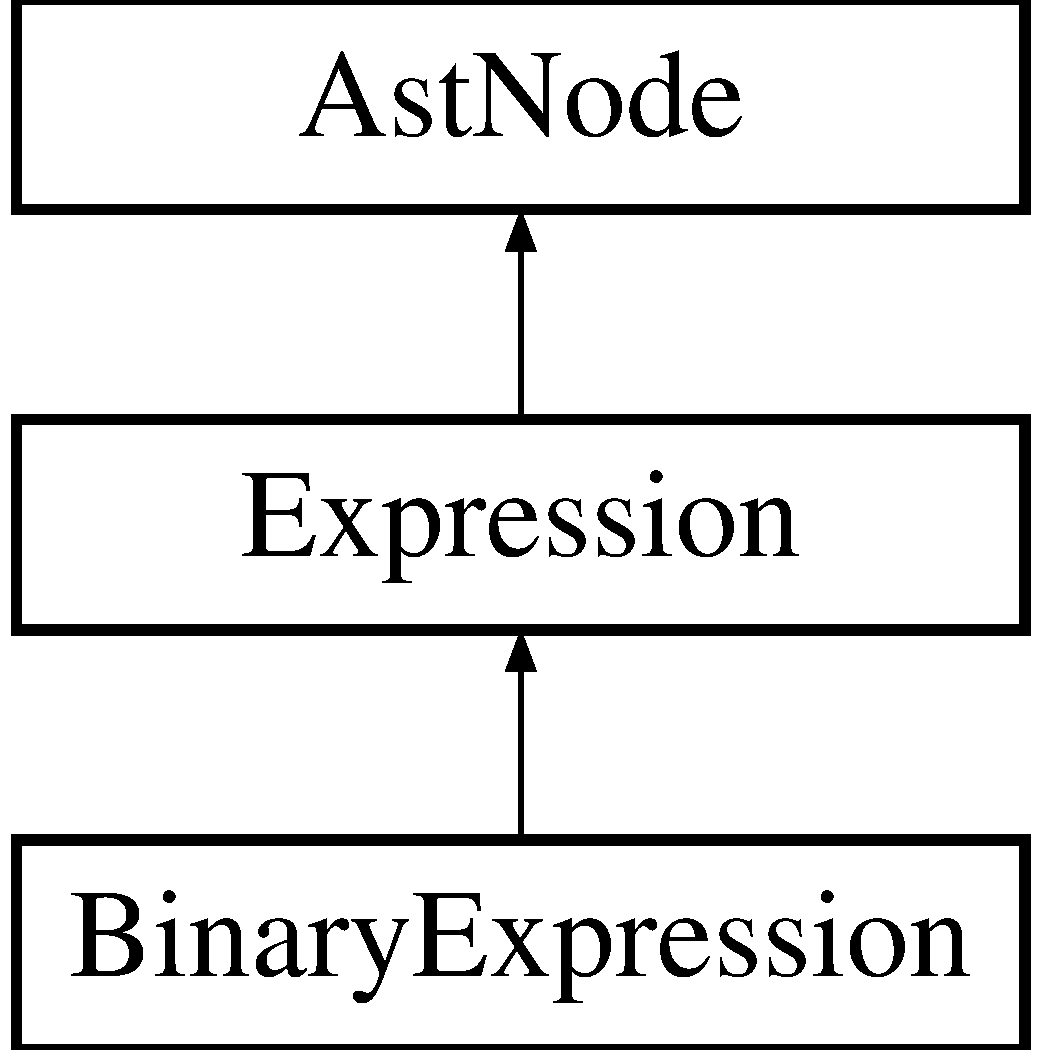
\includegraphics[height=3cm]{classBinaryExpression}
\end{center}
\end{figure}
\subsection*{Public Member Functions}
\begin{DoxyCompactItemize}
\item 
\hyperlink{classBinaryExpression_af36e7f9f5222b93f030748384c631eb0}{BinaryExpression} (int lno, int op, \hyperlink{classExpression}{Expression} $\ast$left, \hyperlink{classExpression}{Expression} $\ast$right)
\item 
int \hyperlink{classBinaryExpression_af2d7644a8e57083fe9c550cf02900068}{getOperator} ()
\item 
\hyperlink{classExpression}{Expression} $\ast$ \hyperlink{classBinaryExpression_a0b8e6e09079d13b029c1fae785e0be01}{getLeftOperand} ()
\item 
\hyperlink{classExpression}{Expression} $\ast$ \hyperlink{classBinaryExpression_a49ee8f4a0fbed5656fbd0c37446e8f82}{getRightOperand} ()
\item 
void \hyperlink{classBinaryExpression_a2bf7fd38f96a775a988bfb6b7838d9bf}{setLeftOperand} (\hyperlink{classExpression}{Expression} $\ast$left)
\item 
void \hyperlink{classBinaryExpression_a78f08f420bbba62af7fc8693bde2fb76}{setRightOperand} (\hyperlink{classExpression}{Expression} $\ast$right)
\item 
void \hyperlink{classBinaryExpression_a2af7e73b6a90c216ef00b6297ce83da5}{accept} (\hyperlink{classAstVisitor}{AstVisitor} $\ast$aVisitor)
\end{DoxyCompactItemize}


\subsection{Detailed Description}
This class represents a TinyJava binary expression involving a binary operator and 2 operand expressions. A binary expression is represented by:
\begin{DoxyItemize}
\item an operator (which may be an arithmetic, relational, or equality operator)
\item a left expression subtree representing the left operand, and
\item a right expression subtree representing the right operand. 
\end{DoxyItemize}

\subsection{Constructor \& Destructor Documentation}
\hypertarget{classBinaryExpression_af36e7f9f5222b93f030748384c631eb0}{
\index{BinaryExpression@{BinaryExpression}!BinaryExpression@{BinaryExpression}}
\index{BinaryExpression@{BinaryExpression}!BinaryExpression@{BinaryExpression}}
\subsubsection[{BinaryExpression}]{\setlength{\rightskip}{0pt plus 5cm}BinaryExpression::BinaryExpression (int {\em lno}, \/  int {\em op}, \/  {\bf Expression} $\ast$ {\em left}, \/  {\bf Expression} $\ast$ {\em right})}}
\label{classBinaryExpression_af36e7f9f5222b93f030748384c631eb0}
Create a new \hyperlink{classBinaryExpression}{BinaryExpression} object.


\begin{DoxyParams}{Parameters}
\item[{\em lno}]source code line number with the binary expression. \item[{\em op}]an int value representing the operator; it should be one of the constants defined in the \hyperlink{classAstNode}{AstNode} class \item[{\em left}]an \hyperlink{classExpression}{Expression} representing the left operand \item[{\em right}]an \hyperlink{classExpression}{Expression} representing the right operand \end{DoxyParams}

\begin{DoxyExceptions}{Exceptions}
\item[{\em \hyperlink{classAstException}{AstException}}]if either the left operand or the right operand is NULL \end{DoxyExceptions}


\subsection{Member Function Documentation}
\hypertarget{classBinaryExpression_a2af7e73b6a90c216ef00b6297ce83da5}{
\index{BinaryExpression@{BinaryExpression}!accept@{accept}}
\index{accept@{accept}!BinaryExpression@{BinaryExpression}}
\subsubsection[{accept}]{\setlength{\rightskip}{0pt plus 5cm}void BinaryExpression::accept ({\bf AstVisitor} $\ast$ {\em aVisitor})\hspace{0.3cm}{\ttfamily  \mbox{[}inline, virtual\mbox{]}}}}
\label{classBinaryExpression_a2af7e73b6a90c216ef00b6297ce83da5}
Accept a visitor to this node. 
\begin{DoxyParams}{Parameters}
\item[{\em aVisitor}]is a visitor object of type \hyperlink{classAstVisitor}{AstVisitor}. \end{DoxyParams}


Implements \hyperlink{classAstNode_a67b2d6ce1262da2954fb4db255759fb3}{AstNode}.\hypertarget{classBinaryExpression_a0b8e6e09079d13b029c1fae785e0be01}{
\index{BinaryExpression@{BinaryExpression}!getLeftOperand@{getLeftOperand}}
\index{getLeftOperand@{getLeftOperand}!BinaryExpression@{BinaryExpression}}
\subsubsection[{getLeftOperand}]{\setlength{\rightskip}{0pt plus 5cm}{\bf Expression}$\ast$ BinaryExpression::getLeftOperand ()\hspace{0.3cm}{\ttfamily  \mbox{[}inline\mbox{]}}}}
\label{classBinaryExpression_a0b8e6e09079d13b029c1fae785e0be01}
Return the left operand of this binary expression.

\begin{DoxyReturn}{Returns}
the \hyperlink{classExpression}{Expression} which is the left operand. 
\end{DoxyReturn}
\hypertarget{classBinaryExpression_af2d7644a8e57083fe9c550cf02900068}{
\index{BinaryExpression@{BinaryExpression}!getOperator@{getOperator}}
\index{getOperator@{getOperator}!BinaryExpression@{BinaryExpression}}
\subsubsection[{getOperator}]{\setlength{\rightskip}{0pt plus 5cm}int BinaryExpression::getOperator ()\hspace{0.3cm}{\ttfamily  \mbox{[}inline\mbox{]}}}}
\label{classBinaryExpression_af2d7644a8e57083fe9c550cf02900068}
Return the operator of this binary expression.

\begin{DoxyReturn}{Returns}
operator as defined in the \hyperlink{classAstNode}{AstNode} class. 
\end{DoxyReturn}
\hypertarget{classBinaryExpression_a49ee8f4a0fbed5656fbd0c37446e8f82}{
\index{BinaryExpression@{BinaryExpression}!getRightOperand@{getRightOperand}}
\index{getRightOperand@{getRightOperand}!BinaryExpression@{BinaryExpression}}
\subsubsection[{getRightOperand}]{\setlength{\rightskip}{0pt plus 5cm}{\bf Expression}$\ast$ BinaryExpression::getRightOperand ()\hspace{0.3cm}{\ttfamily  \mbox{[}inline\mbox{]}}}}
\label{classBinaryExpression_a49ee8f4a0fbed5656fbd0c37446e8f82}
Return the right operand of this binary expression.

\begin{DoxyReturn}{Returns}
the \hyperlink{classExpression}{Expression} which is the right operand. 
\end{DoxyReturn}
\hypertarget{classBinaryExpression_a2bf7fd38f96a775a988bfb6b7838d9bf}{
\index{BinaryExpression@{BinaryExpression}!setLeftOperand@{setLeftOperand}}
\index{setLeftOperand@{setLeftOperand}!BinaryExpression@{BinaryExpression}}
\subsubsection[{setLeftOperand}]{\setlength{\rightskip}{0pt plus 5cm}void BinaryExpression::setLeftOperand ({\bf Expression} $\ast$ {\em left})\hspace{0.3cm}{\ttfamily  \mbox{[}inline\mbox{]}}}}
\label{classBinaryExpression_a2bf7fd38f96a775a988bfb6b7838d9bf}
Set the left operand expression of this binary expression.


\begin{DoxyParams}{Parameters}
\item[{\em left}]the expression to be the new left operand. \end{DoxyParams}

\begin{DoxyExceptions}{Exceptions}
\item[{\em \hyperlink{classAstException}{AstException}}]if the argument is NULL \end{DoxyExceptions}
\hypertarget{classBinaryExpression_a78f08f420bbba62af7fc8693bde2fb76}{
\index{BinaryExpression@{BinaryExpression}!setRightOperand@{setRightOperand}}
\index{setRightOperand@{setRightOperand}!BinaryExpression@{BinaryExpression}}
\subsubsection[{setRightOperand}]{\setlength{\rightskip}{0pt plus 5cm}void BinaryExpression::setRightOperand ({\bf Expression} $\ast$ {\em right})\hspace{0.3cm}{\ttfamily  \mbox{[}inline\mbox{]}}}}
\label{classBinaryExpression_a78f08f420bbba62af7fc8693bde2fb76}
Set the right operand expression of this binary expression.


\begin{DoxyParams}{Parameters}
\item[{\em right}]the expression to be the new right operand. \end{DoxyParams}

\begin{DoxyExceptions}{Exceptions}
\item[{\em \hyperlink{classAstException}{AstException}}]if the argument is NULL \end{DoxyExceptions}


The documentation for this class was generated from the following files:\begin{DoxyCompactItemize}
\item 
BinaryExpression.h\item 
BinaryExpression.cpp\end{DoxyCompactItemize}

\hypertarget{classBlockStatement}{
\section{BlockStatement Class Reference}
\label{classBlockStatement}\index{BlockStatement@{BlockStatement}}
}


This class represents a TinyJave block statement; local variables are not represented within a \hyperlink{classBlockStatement}{BlockStatement}, but with a \hyperlink{classMethodDeclaration}{MethodDeclaration}.  


{\ttfamily \#include $<$BlockStmt.h$>$}Inheritance diagram for BlockStatement::\begin{figure}[H]
\begin{center}
\leavevmode
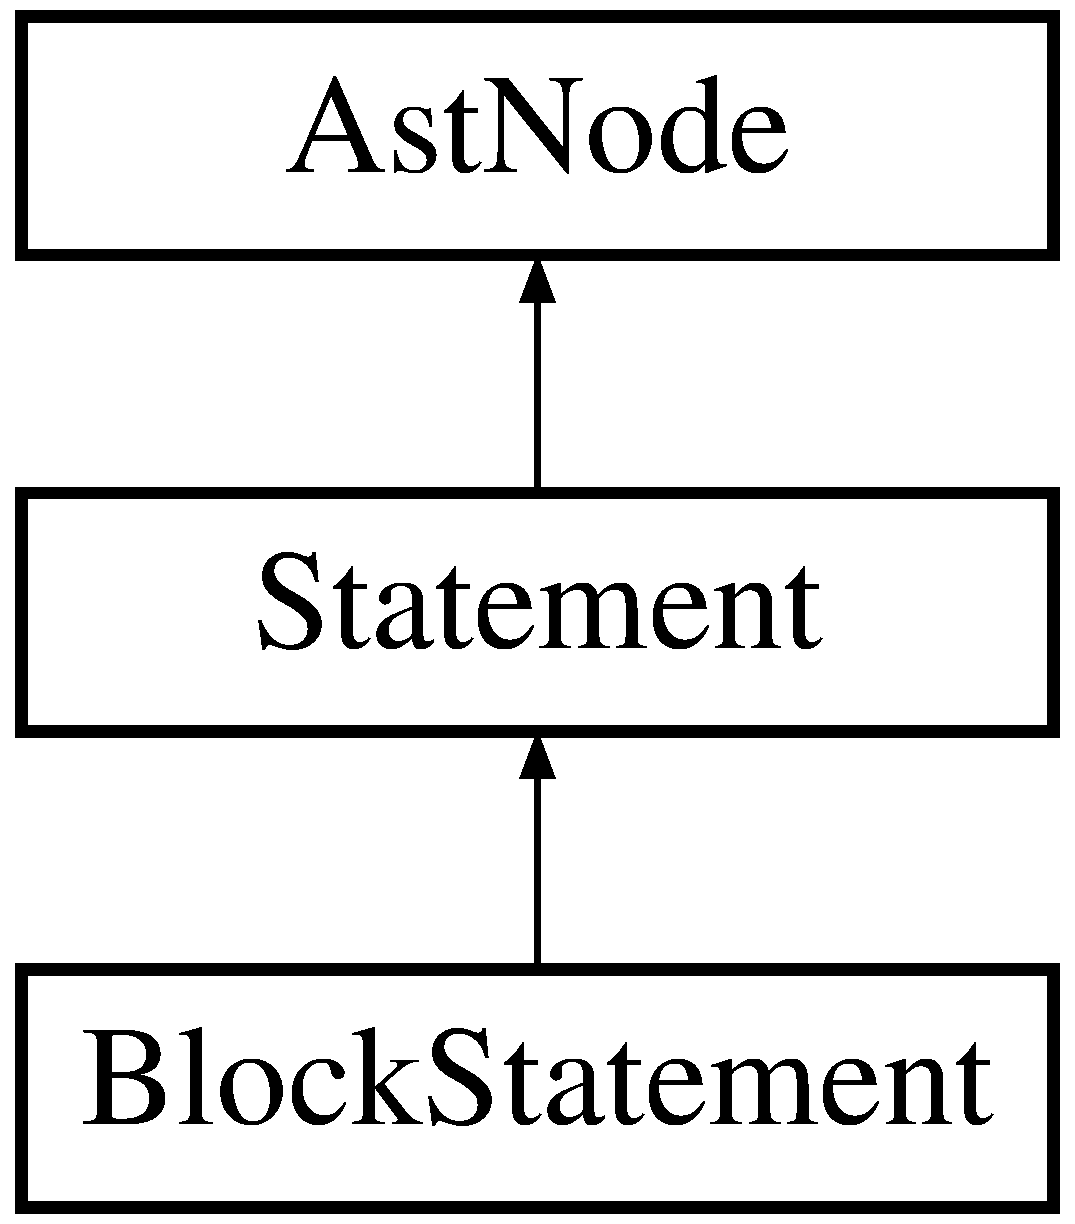
\includegraphics[height=3cm]{classBlockStatement}
\end{center}
\end{figure}
\subsection*{Public Member Functions}
\begin{DoxyCompactItemize}
\item 
\hyperlink{classBlockStatement_a7d28cb688a765ca809bc55aa75e0b245}{BlockStatement} (int lno)
\item 
std::vector$<$ \hyperlink{classStatement}{Statement} $\ast$ $>$ $\ast$ \hyperlink{classBlockStatement_a049f6ad899e8480dd3b55bab8f442928}{getStatements} ()
\item 
void \hyperlink{classBlockStatement_adbd315994e8319333c0f7cd22681ec31}{addStatement} (\hyperlink{classStatement}{Statement} $\ast$stmt)
\item 
void \hyperlink{classBlockStatement_a36f2db846cf7f7a559e8b19b5e3d5c01}{prependStatement} (\hyperlink{classStatement}{Statement} $\ast$stmt)
\item 
void \hyperlink{classBlockStatement_a20df05e7536e375226639b483e8c4732}{accept} (\hyperlink{classAstVisitor}{AstVisitor} $\ast$aVisitor)
\end{DoxyCompactItemize}


\subsection{Detailed Description}
This class represents a TinyJave block statement; local variables are not represented within a \hyperlink{classBlockStatement}{BlockStatement}, but with a \hyperlink{classMethodDeclaration}{MethodDeclaration}. A block statement is a sequence of statements represented as a std::vector of \hyperlink{classStatement}{Statement} nodes. 

\subsection{Constructor \& Destructor Documentation}
\hypertarget{classBlockStatement_a7d28cb688a765ca809bc55aa75e0b245}{
\index{BlockStatement@{BlockStatement}!BlockStatement@{BlockStatement}}
\index{BlockStatement@{BlockStatement}!BlockStatement@{BlockStatement}}
\subsubsection[{BlockStatement}]{\setlength{\rightskip}{0pt plus 5cm}BlockStatement::BlockStatement (int {\em lno})}}
\label{classBlockStatement_a7d28cb688a765ca809bc55aa75e0b245}
Create a new block statement node.


\begin{DoxyParams}{Parameters}
\item[{\em lno}]is a source line number (should be the beginning of the block). \end{DoxyParams}


\subsection{Member Function Documentation}
\hypertarget{classBlockStatement_a20df05e7536e375226639b483e8c4732}{
\index{BlockStatement@{BlockStatement}!accept@{accept}}
\index{accept@{accept}!BlockStatement@{BlockStatement}}
\subsubsection[{accept}]{\setlength{\rightskip}{0pt plus 5cm}void BlockStatement::accept ({\bf AstVisitor} $\ast$ {\em aVisitor})\hspace{0.3cm}{\ttfamily  \mbox{[}inline, virtual\mbox{]}}}}
\label{classBlockStatement_a20df05e7536e375226639b483e8c4732}
Accept a visitor to this node. 
\begin{DoxyParams}{Parameters}
\item[{\em aVisitor}]is a visitor object of type \hyperlink{classAstVisitor}{AstVisitor}. \end{DoxyParams}


Implements \hyperlink{classAstNode_a67b2d6ce1262da2954fb4db255759fb3}{AstNode}.\hypertarget{classBlockStatement_adbd315994e8319333c0f7cd22681ec31}{
\index{BlockStatement@{BlockStatement}!addStatement@{addStatement}}
\index{addStatement@{addStatement}!BlockStatement@{BlockStatement}}
\subsubsection[{addStatement}]{\setlength{\rightskip}{0pt plus 5cm}void BlockStatement::addStatement ({\bf Statement} $\ast$ {\em stmt})}}
\label{classBlockStatement_adbd315994e8319333c0f7cd22681ec31}
Add a statement to this block statement at the end.


\begin{DoxyParams}{Parameters}
\item[{\em stmt}]a \hyperlink{classStatement}{Statement} to be aded as the last in sequence. \end{DoxyParams}

\begin{DoxyExceptions}{Exceptions}
\item[{\em \hyperlink{classAstException}{AstException}}]if the argument is NULL \end{DoxyExceptions}
\hypertarget{classBlockStatement_a049f6ad899e8480dd3b55bab8f442928}{
\index{BlockStatement@{BlockStatement}!getStatements@{getStatements}}
\index{getStatements@{getStatements}!BlockStatement@{BlockStatement}}
\subsubsection[{getStatements}]{\setlength{\rightskip}{0pt plus 5cm}std::vector$<${\bf Statement} $\ast$$>$$\ast$ BlockStatement::getStatements ()\hspace{0.3cm}{\ttfamily  \mbox{[}inline\mbox{]}}}}
\label{classBlockStatement_a049f6ad899e8480dd3b55bab8f442928}
Return the statements of this block.

\begin{DoxyReturn}{Returns}
a pointer to the std::vector with the \hyperlink{classStatement}{Statement} nodes 
\end{DoxyReturn}
\hypertarget{classBlockStatement_a36f2db846cf7f7a559e8b19b5e3d5c01}{
\index{BlockStatement@{BlockStatement}!prependStatement@{prependStatement}}
\index{prependStatement@{prependStatement}!BlockStatement@{BlockStatement}}
\subsubsection[{prependStatement}]{\setlength{\rightskip}{0pt plus 5cm}void BlockStatement::prependStatement ({\bf Statement} $\ast$ {\em stmt})}}
\label{classBlockStatement_a36f2db846cf7f7a559e8b19b5e3d5c01}
Add another statement to this block statement in the front.


\begin{DoxyParams}{Parameters}
\item[{\em stmt}]a \hyperlink{classStatement}{Statement} to be aded as the first in sequence. \end{DoxyParams}

\begin{DoxyExceptions}{Exceptions}
\item[{\em \hyperlink{classAstException}{AstException}}]if the argument is NULL \end{DoxyExceptions}


The documentation for this class was generated from the following files:\begin{DoxyCompactItemize}
\item 
BlockStmt.h\item 
BlockStmt.cpp\end{DoxyCompactItemize}

\hypertarget{classCastExpression}{
\section{CastExpression Class Reference}
\label{classCastExpression}\index{CastExpression@{CastExpression}}
}


This class represents a TinyJava type cast expression.  


{\ttfamily \#include $<$CastExpression.h$>$}Inheritance diagram for CastExpression::\begin{figure}[H]
\begin{center}
\leavevmode
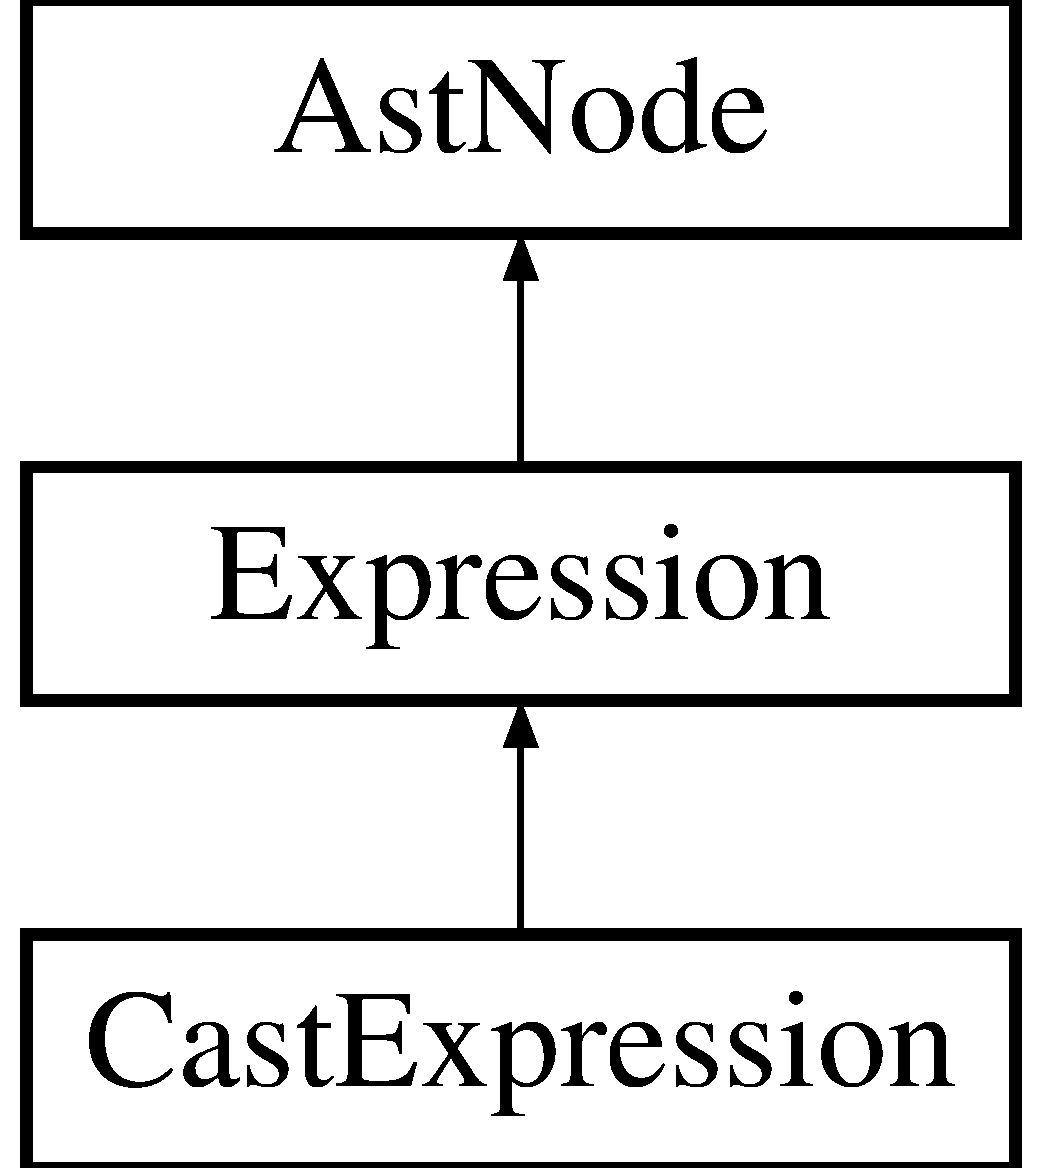
\includegraphics[height=3cm]{classCastExpression}
\end{center}
\end{figure}
\subsection*{Public Member Functions}
\begin{DoxyCompactItemize}
\item 
\hyperlink{classCastExpression_a1c5bdbe92eabf17c09577c39937f4ff0}{CastExpression} (int lno, int castToType, \hyperlink{classExpression}{Expression} $\ast$arg)
\item 
int \hyperlink{classCastExpression_aa6ba133577fc9296450cb88410a24853}{getCastToType} ()
\item 
void \hyperlink{classCastExpression_ae0d08e3b57a33740d1d85f283ed755ab}{setCastToType} (int ct)
\item 
\hyperlink{classExpression}{Expression} $\ast$ \hyperlink{classCastExpression_ac35b327f25747795273b7bf991c77eef}{getOperand} ()
\item 
void \hyperlink{classCastExpression_ac24a64d42327406feeee20ef0b641c6b}{setOperand} (\hyperlink{classExpression}{Expression} $\ast$arg)
\item 
void \hyperlink{classCastExpression_af98e34f83dce5fec6d21f4baf4679dea}{accept} (\hyperlink{classAstVisitor}{AstVisitor} $\ast$aVisitor)
\end{DoxyCompactItemize}


\subsection{Detailed Description}
This class represents a TinyJava type cast expression. A cast expression is represented by:
\begin{DoxyItemize}
\item the resulting type (an integer, as defined in the \hyperlink{classAstNode}{AstNode} class)
\item the \hyperlink{classExpression}{Expression} whose result should be type cast. 
\end{DoxyItemize}

\subsection{Constructor \& Destructor Documentation}
\hypertarget{classCastExpression_a1c5bdbe92eabf17c09577c39937f4ff0}{
\index{CastExpression@{CastExpression}!CastExpression@{CastExpression}}
\index{CastExpression@{CastExpression}!CastExpression@{CastExpression}}
\subsubsection[{CastExpression}]{\setlength{\rightskip}{0pt plus 5cm}CastExpression::CastExpression (int {\em lno}, \/  int {\em castToType}, \/  {\bf Expression} $\ast$ {\em arg})}}
\label{classCastExpression_a1c5bdbe92eabf17c09577c39937f4ff0}
Create a new \hyperlink{classCastExpression}{CastExpression} object.


\begin{DoxyParams}{Parameters}
\item[{\em lno}]a source code line number with the type cast \item[{\em castToType}]the resulting type (as defined in the \hyperlink{classAstNode}{AstNode} class) \item[{\em arg}]the argument expression to be type cast. \end{DoxyParams}

\begin{DoxyExceptions}{Exceptions}
\item[{\em \hyperlink{classAstException}{AstException}}]if the \hyperlink{classExpression}{Expression} argument is NULL \end{DoxyExceptions}


\subsection{Member Function Documentation}
\hypertarget{classCastExpression_af98e34f83dce5fec6d21f4baf4679dea}{
\index{CastExpression@{CastExpression}!accept@{accept}}
\index{accept@{accept}!CastExpression@{CastExpression}}
\subsubsection[{accept}]{\setlength{\rightskip}{0pt plus 5cm}void CastExpression::accept ({\bf AstVisitor} $\ast$ {\em aVisitor})\hspace{0.3cm}{\ttfamily  \mbox{[}inline, virtual\mbox{]}}}}
\label{classCastExpression_af98e34f83dce5fec6d21f4baf4679dea}
Accept a visitor to this node. 
\begin{DoxyParams}{Parameters}
\item[{\em aVisitor}]is a visitor object of type \hyperlink{classAstVisitor}{AstVisitor}. \end{DoxyParams}


Implements \hyperlink{classAstNode_a67b2d6ce1262da2954fb4db255759fb3}{AstNode}.\hypertarget{classCastExpression_aa6ba133577fc9296450cb88410a24853}{
\index{CastExpression@{CastExpression}!getCastToType@{getCastToType}}
\index{getCastToType@{getCastToType}!CastExpression@{CastExpression}}
\subsubsection[{getCastToType}]{\setlength{\rightskip}{0pt plus 5cm}int CastExpression::getCastToType ()\hspace{0.3cm}{\ttfamily  \mbox{[}inline\mbox{]}}}}
\label{classCastExpression_aa6ba133577fc9296450cb88410a24853}
Return the type of the tape cast expression.

\begin{DoxyReturn}{Returns}
int value representing the type (as defined in the \hyperlink{classAstNode}{AstNode} class) 
\end{DoxyReturn}
\hypertarget{classCastExpression_ac35b327f25747795273b7bf991c77eef}{
\index{CastExpression@{CastExpression}!getOperand@{getOperand}}
\index{getOperand@{getOperand}!CastExpression@{CastExpression}}
\subsubsection[{getOperand}]{\setlength{\rightskip}{0pt plus 5cm}{\bf Expression}$\ast$ CastExpression::getOperand ()\hspace{0.3cm}{\ttfamily  \mbox{[}inline\mbox{]}}}}
\label{classCastExpression_ac35b327f25747795273b7bf991c77eef}
Return the operand expression.

\begin{DoxyReturn}{Returns}
an \hyperlink{classExpression}{Expression} node representing the operand expression. 
\end{DoxyReturn}
\hypertarget{classCastExpression_ae0d08e3b57a33740d1d85f283ed755ab}{
\index{CastExpression@{CastExpression}!setCastToType@{setCastToType}}
\index{setCastToType@{setCastToType}!CastExpression@{CastExpression}}
\subsubsection[{setCastToType}]{\setlength{\rightskip}{0pt plus 5cm}void CastExpression::setCastToType (int {\em ct})\hspace{0.3cm}{\ttfamily  \mbox{[}inline\mbox{]}}}}
\label{classCastExpression_ae0d08e3b57a33740d1d85f283ed755ab}
Set the cast-\/to type.


\begin{DoxyParams}{Parameters}
\item[{\em ct}]cast to be typed to, as defined in the \hyperlink{classAstNode}{AstNode} class \end{DoxyParams}
\hypertarget{classCastExpression_ac24a64d42327406feeee20ef0b641c6b}{
\index{CastExpression@{CastExpression}!setOperand@{setOperand}}
\index{setOperand@{setOperand}!CastExpression@{CastExpression}}
\subsubsection[{setOperand}]{\setlength{\rightskip}{0pt plus 5cm}void CastExpression::setOperand ({\bf Expression} $\ast$ {\em arg})\hspace{0.3cm}{\ttfamily  \mbox{[}inline\mbox{]}}}}
\label{classCastExpression_ac24a64d42327406feeee20ef0b641c6b}
Set the operand expression.


\begin{DoxyParams}{Parameters}
\item[{\em arg}]the new \hyperlink{classExpression}{Expression} node to be set as the operand. \end{DoxyParams}

\begin{DoxyExceptions}{Exceptions}
\item[{\em \hyperlink{classAstException}{AstException}}]if the \hyperlink{classExpression}{Expression} argument is NULL \end{DoxyExceptions}


The documentation for this class was generated from the following files:\begin{DoxyCompactItemize}
\item 
CastExpression.h\item 
CastExpression.cpp\end{DoxyCompactItemize}

\hypertarget{classClassDeclaration}{
\section{ClassDeclaration Class Reference}
\label{classClassDeclaration}\index{ClassDeclaration@{ClassDeclaration}}
}


This class represents a TinyJava class declaration.  


{\ttfamily \#include $<$ClassDeclaration.h$>$}Inheritance diagram for ClassDeclaration::\begin{figure}[H]
\begin{center}
\leavevmode
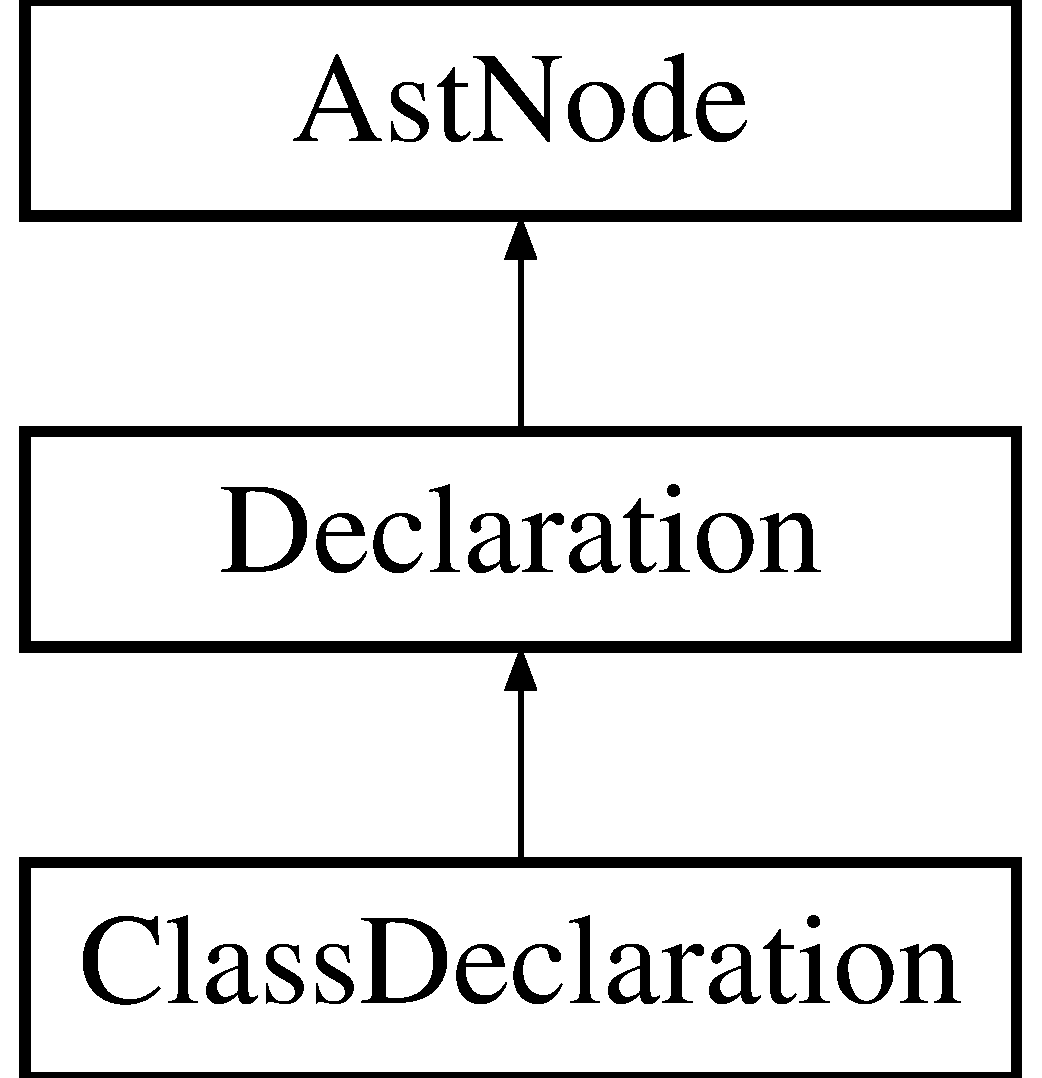
\includegraphics[height=3cm]{classClassDeclaration}
\end{center}
\end{figure}
\subsection*{Public Member Functions}
\begin{DoxyCompactItemize}
\item 
\hyperlink{classClassDeclaration_a1016b2f9166666f12ff69d8f35c5f4b0}{ClassDeclaration} (int lno, const char $\ast$className)
\item 
const char $\ast$ \hyperlink{classClassDeclaration_aee9941ff0bc3f063352dc9150c8f4733}{getName} ()
\item 
void \hyperlink{classClassDeclaration_a4d48dcc425315c542f1bee48287fb237}{addMember} (\hyperlink{classDeclaration}{Declaration} $\ast$member)
\item 
int \hyperlink{classClassDeclaration_ae2b6695aa4eee03d8516637535ec4907}{getNoMembers} ()
\item 
\hyperlink{classDeclaration}{Declaration} $\ast$ \hyperlink{classClassDeclaration_a2a905ef9d8d1034606f554917c1a83f6}{getMember} (int pos)
\item 
std::vector$<$ \hyperlink{classDeclaration}{Declaration} $\ast$ $>$ $\ast$ \hyperlink{classClassDeclaration_ac52a79fdbdf26dd21327c54632d9d452}{getMembers} ()
\item 
void \hyperlink{classClassDeclaration_abb1e806c4c54cfecbc685b5c8a072eae}{accept} (\hyperlink{classAstVisitor}{AstVisitor} $\ast$aVisitor)
\end{DoxyCompactItemize}


\subsection{Detailed Description}
This class represents a TinyJava class declaration. A class declaration is represented by:
\begin{DoxyItemize}
\item a string representing the class name
\item a list of class members, that is fields and methods, represented by \hyperlink{classFieldDeclaration}{FieldDeclaration} and \hyperlink{classMethodDeclaration}{MethodDeclaration} nodes, respectively. 
\end{DoxyItemize}

\subsection{Constructor \& Destructor Documentation}
\hypertarget{classClassDeclaration_a1016b2f9166666f12ff69d8f35c5f4b0}{
\index{ClassDeclaration@{ClassDeclaration}!ClassDeclaration@{ClassDeclaration}}
\index{ClassDeclaration@{ClassDeclaration}!ClassDeclaration@{ClassDeclaration}}
\subsubsection[{ClassDeclaration}]{\setlength{\rightskip}{0pt plus 5cm}ClassDeclaration::ClassDeclaration (int {\em lno}, \/  const char $\ast$ {\em className})}}
\label{classClassDeclaration_a1016b2f9166666f12ff69d8f35c5f4b0}
Create a new \hyperlink{classClassDeclaration}{ClassDeclaration} object.


\begin{DoxyParams}{Parameters}
\item[{\em lno}]a source code line number (should be the start of the class declaration). \item[{\em className}]a string with the class name \end{DoxyParams}


\subsection{Member Function Documentation}
\hypertarget{classClassDeclaration_abb1e806c4c54cfecbc685b5c8a072eae}{
\index{ClassDeclaration@{ClassDeclaration}!accept@{accept}}
\index{accept@{accept}!ClassDeclaration@{ClassDeclaration}}
\subsubsection[{accept}]{\setlength{\rightskip}{0pt plus 5cm}void ClassDeclaration::accept ({\bf AstVisitor} $\ast$ {\em aVisitor})\hspace{0.3cm}{\ttfamily  \mbox{[}inline, virtual\mbox{]}}}}
\label{classClassDeclaration_abb1e806c4c54cfecbc685b5c8a072eae}
Accept a visitor to this node. 
\begin{DoxyParams}{Parameters}
\item[{\em aVisitor}]is a visitor object of type \hyperlink{classAstVisitor}{AstVisitor}. \end{DoxyParams}


Implements \hyperlink{classAstNode_a67b2d6ce1262da2954fb4db255759fb3}{AstNode}.\hypertarget{classClassDeclaration_a4d48dcc425315c542f1bee48287fb237}{
\index{ClassDeclaration@{ClassDeclaration}!addMember@{addMember}}
\index{addMember@{addMember}!ClassDeclaration@{ClassDeclaration}}
\subsubsection[{addMember}]{\setlength{\rightskip}{0pt plus 5cm}void ClassDeclaration::addMember ({\bf Declaration} $\ast$ {\em member})}}
\label{classClassDeclaration_a4d48dcc425315c542f1bee48287fb237}
Add a new class mamber (either a field or a method).


\begin{DoxyParams}{Parameters}
\item[{\em member}]a \hyperlink{classDeclaration}{Declaration} node representing the new class member. It must be either a pointer to \hyperlink{classFieldDeclaration}{FieldDeclaration} or to \hyperlink{classMethodDeclaration}{MethodDeclaration}. \end{DoxyParams}

\begin{DoxyExceptions}{Exceptions}
\item[{\em \hyperlink{classAstException}{AstException}}]if the argument is neither a \hyperlink{classFieldDeclaration}{FieldDeclaration} nor a \hyperlink{classMethodDeclaration}{MethodDeclaration}. \end{DoxyExceptions}
\hypertarget{classClassDeclaration_a2a905ef9d8d1034606f554917c1a83f6}{
\index{ClassDeclaration@{ClassDeclaration}!getMember@{getMember}}
\index{getMember@{getMember}!ClassDeclaration@{ClassDeclaration}}
\subsubsection[{getMember}]{\setlength{\rightskip}{0pt plus 5cm}{\bf Declaration}$\ast$ ClassDeclaration::getMember (int {\em pos})\hspace{0.3cm}{\ttfamily  \mbox{[}inline\mbox{]}}}}
\label{classClassDeclaration_a2a905ef9d8d1034606f554917c1a83f6}
Return the i-\/the class member.


\begin{DoxyParams}{Parameters}
\item[{\em pos}]integer representing the position of the class member requested. \end{DoxyParams}
\begin{DoxyReturn}{Returns}
a pointer to a \hyperlink{classDeclaration}{Declaration} representing the requested class member. 
\end{DoxyReturn}

\begin{DoxyExceptions}{Exceptions}
\item[{\em \hyperlink{classAstException}{AstException}}]if there are no members or if the pos value is out of bounds \end{DoxyExceptions}
\hypertarget{classClassDeclaration_ac52a79fdbdf26dd21327c54632d9d452}{
\index{ClassDeclaration@{ClassDeclaration}!getMembers@{getMembers}}
\index{getMembers@{getMembers}!ClassDeclaration@{ClassDeclaration}}
\subsubsection[{getMembers}]{\setlength{\rightskip}{0pt plus 5cm}std::vector$<${\bf Declaration} $\ast$$>$$\ast$ ClassDeclaration::getMembers ()\hspace{0.3cm}{\ttfamily  \mbox{[}inline\mbox{]}}}}
\label{classClassDeclaration_ac52a79fdbdf26dd21327c54632d9d452}
Return all class members.

\begin{DoxyReturn}{Returns}
a pointer to a std::vector representing all class members in this class declaration. 
\end{DoxyReturn}
\hypertarget{classClassDeclaration_aee9941ff0bc3f063352dc9150c8f4733}{
\index{ClassDeclaration@{ClassDeclaration}!getName@{getName}}
\index{getName@{getName}!ClassDeclaration@{ClassDeclaration}}
\subsubsection[{getName}]{\setlength{\rightskip}{0pt plus 5cm}const char$\ast$ ClassDeclaration::getName ()\hspace{0.3cm}{\ttfamily  \mbox{[}inline\mbox{]}}}}
\label{classClassDeclaration_aee9941ff0bc3f063352dc9150c8f4733}
Return the class name.

\begin{DoxyReturn}{Returns}
string representing the class name. 
\end{DoxyReturn}
\hypertarget{classClassDeclaration_ae2b6695aa4eee03d8516637535ec4907}{
\index{ClassDeclaration@{ClassDeclaration}!getNoMembers@{getNoMembers}}
\index{getNoMembers@{getNoMembers}!ClassDeclaration@{ClassDeclaration}}
\subsubsection[{getNoMembers}]{\setlength{\rightskip}{0pt plus 5cm}int ClassDeclaration::getNoMembers ()\hspace{0.3cm}{\ttfamily  \mbox{[}inline\mbox{]}}}}
\label{classClassDeclaration_ae2b6695aa4eee03d8516637535ec4907}
Return the number of class members in this \hyperlink{classClassDeclaration}{ClassDeclaration} node.

\begin{DoxyReturn}{Returns}
the number of class members. 
\end{DoxyReturn}


The documentation for this class was generated from the following files:\begin{DoxyCompactItemize}
\item 
ClassDeclaration.h\item 
ClassDeclaration.cpp\end{DoxyCompactItemize}

\hypertarget{classDeclaration}{
\section{Declaration Class Reference}
\label{classDeclaration}\index{Declaration@{Declaration}}
}


This is the parent of all declaration Abstract Syntax Tree nodes.  


{\ttfamily \#include $<$Declaration.h$>$}Inheritance diagram for Declaration::\begin{figure}[H]
\begin{center}
\leavevmode
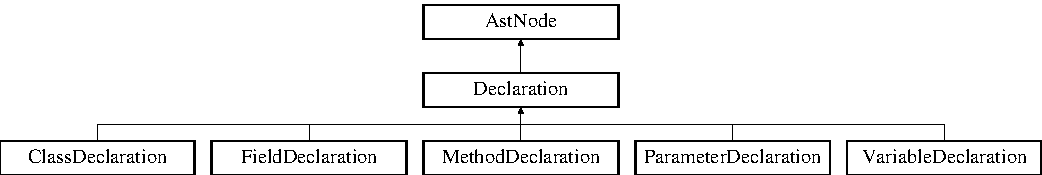
\includegraphics[height=2.34965cm]{classDeclaration}
\end{center}
\end{figure}


\subsection{Detailed Description}
This is the parent of all declaration Abstract Syntax Tree nodes. This class will not have direct instances. It only serves as the common parent class of:


\begin{DoxyItemize}
\item \hyperlink{classClassDeclaration}{ClassDeclaration},
\item FieldDeclarations,
\item \hyperlink{classMethodDeclaration}{MethodDeclaration},
\item \hyperlink{classParameterDeclaration}{ParameterDeclaration}, and
\item \hyperlink{classVariableDeclaration}{VariableDeclaration} 
\end{DoxyItemize}

The documentation for this class was generated from the following file:\begin{DoxyCompactItemize}
\item 
Declaration.h\end{DoxyCompactItemize}

\hypertarget{classEmptyStatement}{
\section{EmptyStatement Class Reference}
\label{classEmptyStatement}\index{EmptyStatement@{EmptyStatement}}
}


This class represents a TinyJava empty statement.  


{\ttfamily \#include $<$EmptyStmt.h$>$}Inheritance diagram for EmptyStatement::\begin{figure}[H]
\begin{center}
\leavevmode
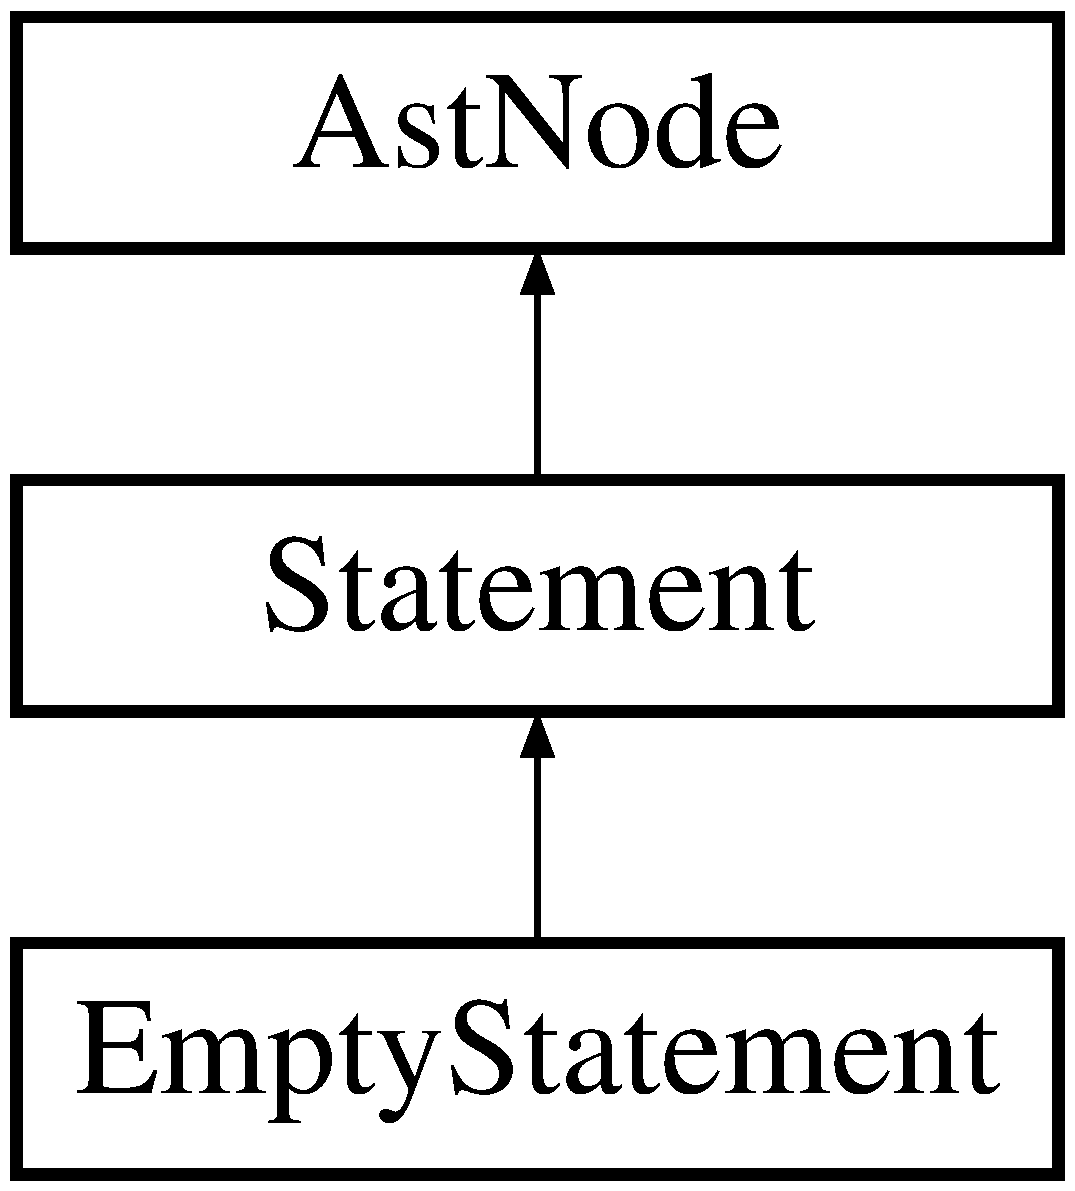
\includegraphics[height=3cm]{classEmptyStatement}
\end{center}
\end{figure}
\subsection*{Public Member Functions}
\begin{DoxyCompactItemize}
\item 
\hyperlink{classEmptyStatement_a95dfede9144f6f66b6ded4497147ec16}{EmptyStatement} (int lno)
\item 
void \hyperlink{classEmptyStatement_a54138a042d8de2fecf90448a0048757b}{accept} (\hyperlink{classAstVisitor}{AstVisitor} $\ast$aVisitor)
\end{DoxyCompactItemize}


\subsection{Detailed Description}
This class represents a TinyJava empty statement. 

\subsection{Constructor \& Destructor Documentation}
\hypertarget{classEmptyStatement_a95dfede9144f6f66b6ded4497147ec16}{
\index{EmptyStatement@{EmptyStatement}!EmptyStatement@{EmptyStatement}}
\index{EmptyStatement@{EmptyStatement}!EmptyStatement@{EmptyStatement}}
\subsubsection[{EmptyStatement}]{\setlength{\rightskip}{0pt plus 5cm}EmptyStatement::EmptyStatement (int {\em lno})\hspace{0.3cm}{\ttfamily  \mbox{[}inline\mbox{]}}}}
\label{classEmptyStatement_a95dfede9144f6f66b6ded4497147ec16}
Create a \hyperlink{classEmptyStatement}{EmptyStatement} object.


\begin{DoxyParams}{Parameters}
\item[{\em lno}]a source code line number with the empty statement. \end{DoxyParams}


\subsection{Member Function Documentation}
\hypertarget{classEmptyStatement_a54138a042d8de2fecf90448a0048757b}{
\index{EmptyStatement@{EmptyStatement}!accept@{accept}}
\index{accept@{accept}!EmptyStatement@{EmptyStatement}}
\subsubsection[{accept}]{\setlength{\rightskip}{0pt plus 5cm}void EmptyStatement::accept ({\bf AstVisitor} $\ast$ {\em aVisitor})\hspace{0.3cm}{\ttfamily  \mbox{[}inline, virtual\mbox{]}}}}
\label{classEmptyStatement_a54138a042d8de2fecf90448a0048757b}
Accept a visitor to this node. 
\begin{DoxyParams}{Parameters}
\item[{\em aVisitor}]is a visitor object of type \hyperlink{classAstVisitor}{AstVisitor}. \end{DoxyParams}


Implements \hyperlink{classAstNode_a67b2d6ce1262da2954fb4db255759fb3}{AstNode}.

The documentation for this class was generated from the following file:\begin{DoxyCompactItemize}
\item 
EmptyStmt.h\end{DoxyCompactItemize}

\hypertarget{classExpression}{
\section{Expression Class Reference}
\label{classExpression}\index{Expression@{Expression}}
}


This is the parent of all expression Abstract Syntax Tree nodes.  


{\ttfamily \#include $<$Expression.h$>$}Inheritance diagram for Expression::\begin{figure}[H]
\begin{center}
\leavevmode
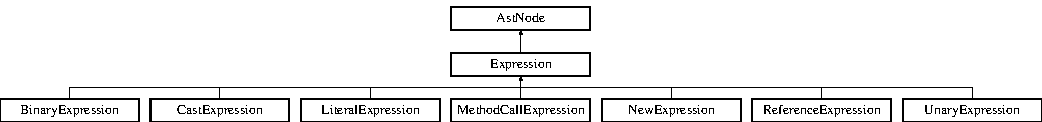
\includegraphics[height=1.64384cm]{classExpression}
\end{center}
\end{figure}
\subsection*{Public Member Functions}
\begin{DoxyCompactItemize}
\item 
\hyperlink{classExpression_afcf87716bf0abfe8d414c92529e1564a}{Expression} ()
\item 
\hyperlink{classExpression_a3b3e124dd46ae70e1aae195089e839ab}{Expression} (int tp)
\item 
int \hyperlink{classExpression_add42721451cd946ac4e02ced146b95b7}{getType} ()
\item 
void \hyperlink{classExpression_ac2a2e67e764dd3ed9733b9cfd3e27f26}{setType} (int tp)
\end{DoxyCompactItemize}


\subsection{Detailed Description}
This is the parent of all expression Abstract Syntax Tree nodes. This class will not have direct instances. Each \hyperlink{classExpression}{Expression} has a type, represented as an integer value, as defined in the \hyperlink{classAstNode}{AstNode} class.

The \hyperlink{classExpression}{Expression} class serves as the common parent class of:


\begin{DoxyItemize}
\item \hyperlink{classReferenceExpression}{ReferenceExpression}
\item \hyperlink{classLiteralExpression}{LiteralExpression}
\item \hyperlink{classNewExpression}{NewExpression}
\item \hyperlink{classMethodCallExpression}{MethodCallExpression}
\item \hyperlink{classCastExpression}{CastExpression}
\item \hyperlink{classUnaryExpression}{UnaryExpression}, and
\item \hyperlink{classBinaryExpression}{BinaryExpression} 
\end{DoxyItemize}

\subsection{Constructor \& Destructor Documentation}
\hypertarget{classExpression_afcf87716bf0abfe8d414c92529e1564a}{
\index{Expression@{Expression}!Expression@{Expression}}
\index{Expression@{Expression}!Expression@{Expression}}
\subsubsection[{Expression}]{\setlength{\rightskip}{0pt plus 5cm}Expression::Expression ()\hspace{0.3cm}{\ttfamily  \mbox{[}inline\mbox{]}}}}
\label{classExpression_afcf87716bf0abfe8d414c92529e1564a}
Create a new \hyperlink{classExpression}{Expression} object. The type will be set to TINT. \hypertarget{classExpression_a3b3e124dd46ae70e1aae195089e839ab}{
\index{Expression@{Expression}!Expression@{Expression}}
\index{Expression@{Expression}!Expression@{Expression}}
\subsubsection[{Expression}]{\setlength{\rightskip}{0pt plus 5cm}Expression::Expression (int {\em tp})\hspace{0.3cm}{\ttfamily  \mbox{[}inline\mbox{]}}}}
\label{classExpression_a3b3e124dd46ae70e1aae195089e839ab}
Create a new \hyperlink{classExpression}{Expression} object.


\begin{DoxyParams}{Parameters}
\item[{\em tp}]the type of the \hyperlink{classExpression}{Expression}. It must be an integer value, as defined in the \hyperlink{classAstNode}{AstNode} class. \end{DoxyParams}


\subsection{Member Function Documentation}
\hypertarget{classExpression_add42721451cd946ac4e02ced146b95b7}{
\index{Expression@{Expression}!getType@{getType}}
\index{getType@{getType}!Expression@{Expression}}
\subsubsection[{getType}]{\setlength{\rightskip}{0pt plus 5cm}int Expression::getType ()\hspace{0.3cm}{\ttfamily  \mbox{[}inline\mbox{]}}}}
\label{classExpression_add42721451cd946ac4e02ced146b95b7}
Return the type of this \hyperlink{classExpression}{Expression} node.

\begin{DoxyReturn}{Returns}
an integer value representing the type, as defined in the \hyperlink{classAstNode}{AstNode} class. 
\end{DoxyReturn}
\hypertarget{classExpression_ac2a2e67e764dd3ed9733b9cfd3e27f26}{
\index{Expression@{Expression}!setType@{setType}}
\index{setType@{setType}!Expression@{Expression}}
\subsubsection[{setType}]{\setlength{\rightskip}{0pt plus 5cm}void Expression::setType (int {\em tp})\hspace{0.3cm}{\ttfamily  \mbox{[}inline\mbox{]}}}}
\label{classExpression_ac2a2e67e764dd3ed9733b9cfd3e27f26}
Set the type of this \hyperlink{classExpression}{Expression} node.


\begin{DoxyParams}{Parameters}
\item[{\em tp}]an integer value representing the type, as defined in the \hyperlink{classAstNode}{AstNode} class. \end{DoxyParams}


The documentation for this class was generated from the following file:\begin{DoxyCompactItemize}
\item 
Expression.h\end{DoxyCompactItemize}

\hypertarget{classFieldDeclaration}{
\section{FieldDeclaration Class Reference}
\label{classFieldDeclaration}\index{FieldDeclaration@{FieldDeclaration}}
}


This class represents a field declaration in a TinyJava class.  


{\ttfamily \#include $<$FieldDeclaration.h$>$}Inheritance diagram for FieldDeclaration::\begin{figure}[H]
\begin{center}
\leavevmode
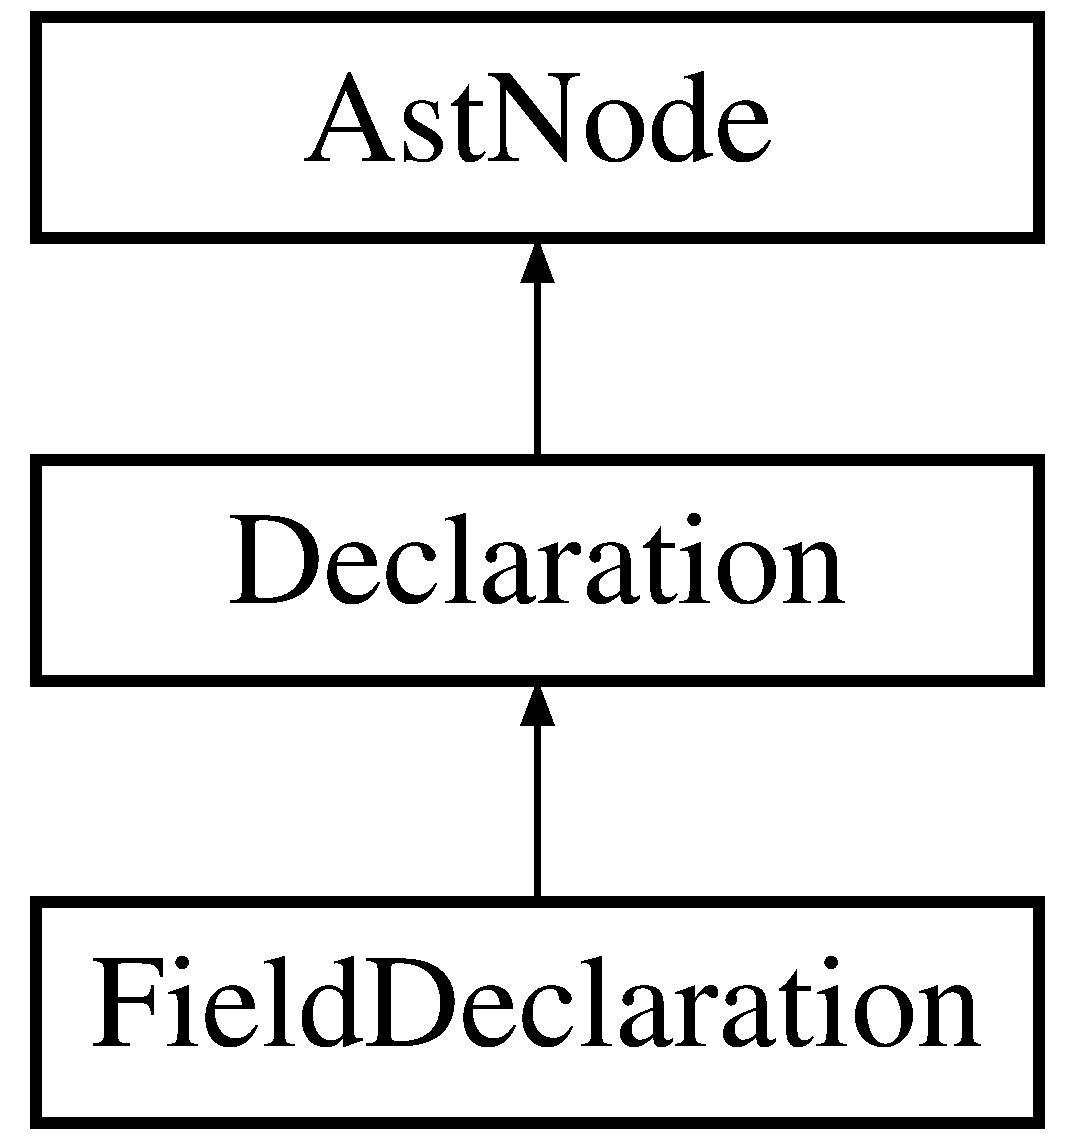
\includegraphics[height=3cm]{classFieldDeclaration}
\end{center}
\end{figure}
\subsection*{Public Member Functions}
\begin{DoxyCompactItemize}
\item 
\hyperlink{classFieldDeclaration_ae9f21a335682f2c26688c8edaf9881e6}{FieldDeclaration} (int lno, const char $\ast$fieldName, int tp, const char $\ast$iv)
\item 
const char $\ast$ \hyperlink{classFieldDeclaration_a132a85e17482895ac3af743eca97b2c4}{getName} ()
\item 
void \hyperlink{classFieldDeclaration_a960feae9f9db3bda2fb1ff5d410c3613}{setName} (const char $\ast$nm)
\item 
int \hyperlink{classFieldDeclaration_af7bf6c60c56fbe7e8e27e470fb6ff870}{getType} ()
\item 
void \hyperlink{classFieldDeclaration_a0dd7650a679bfa235441789848a54740}{setType} (int tp)
\item 
const char $\ast$ \hyperlink{classFieldDeclaration_afaef5c16cd739826c2e1463666690e95}{getInitValue} ()
\item 
void \hyperlink{classFieldDeclaration_a7b9500c22fec4f983f696751a2581fa7}{setInitValue} (const char $\ast$iv)
\item 
ENTRY $\ast$ \hyperlink{classFieldDeclaration_a133d01ba5677049a2fb8eeebc91229c0}{getEntry} ()
\item 
void \hyperlink{classFieldDeclaration_a0220f27540af855ca7c7803728926fb5}{setEntry} (ENTRY $\ast$e)
\item 
void \hyperlink{classFieldDeclaration_a60ce09d75a5864803ca3b24530267af1}{accept} (\hyperlink{classAstVisitor}{AstVisitor} $\ast$aVisitor)
\end{DoxyCompactItemize}


\subsection{Detailed Description}
This class represents a field declaration in a TinyJava class. A class field is represented by:
\begin{DoxyItemize}
\item field name -\/ a string
\item type -\/ an integer value, as defined in the \hyperlink{classAstNode}{AstNode} class
\item initial value -\/ a string representing the initial value literal
\item a pointer to the symbol table ENTRY for the field may be provided, as well.
\end{DoxyItemize}

ENTRY should be defined as a macro, and its value should be a class, which is the root of the symbol table entry hierarchy. Its default value is Entry. The macro should be defined at the beginning of the header file Ast.h. 

\subsection{Constructor \& Destructor Documentation}
\hypertarget{classFieldDeclaration_ae9f21a335682f2c26688c8edaf9881e6}{
\index{FieldDeclaration@{FieldDeclaration}!FieldDeclaration@{FieldDeclaration}}
\index{FieldDeclaration@{FieldDeclaration}!FieldDeclaration@{FieldDeclaration}}
\subsubsection[{FieldDeclaration}]{\setlength{\rightskip}{0pt plus 5cm}FieldDeclaration::FieldDeclaration (int {\em lno}, \/  const char $\ast$ {\em fieldName}, \/  int {\em tp}, \/  const char $\ast$ {\em iv})\hspace{0.3cm}{\ttfamily  \mbox{[}inline\mbox{]}}}}
\label{classFieldDeclaration_ae9f21a335682f2c26688c8edaf9881e6}
Create a new \hyperlink{classFieldDeclaration}{FieldDeclaration} object.


\begin{DoxyParams}{Parameters}
\item[{\em lno}]a source code line number with the field declaration. \item[{\em fieldName}]a string with the field name \item[{\em tp}]an integer representing the type, as defined in the \hyperlink{classAstNode}{AstNode} class \item[{\em iv}]a string with the initial value literal. \end{DoxyParams}

\begin{DoxyExceptions}{Exceptions}
\item[{\em \hyperlink{classAstException}{AstException}}]if the fieldName or the initial value is NULL \end{DoxyExceptions}


\subsection{Member Function Documentation}
\hypertarget{classFieldDeclaration_a60ce09d75a5864803ca3b24530267af1}{
\index{FieldDeclaration@{FieldDeclaration}!accept@{accept}}
\index{accept@{accept}!FieldDeclaration@{FieldDeclaration}}
\subsubsection[{accept}]{\setlength{\rightskip}{0pt plus 5cm}void FieldDeclaration::accept ({\bf AstVisitor} $\ast$ {\em aVisitor})\hspace{0.3cm}{\ttfamily  \mbox{[}inline, virtual\mbox{]}}}}
\label{classFieldDeclaration_a60ce09d75a5864803ca3b24530267af1}
Accept a visitor to this node. 
\begin{DoxyParams}{Parameters}
\item[{\em aVisitor}]is a visitor object of type \hyperlink{classAstVisitor}{AstVisitor}. \end{DoxyParams}


Implements \hyperlink{classAstNode_a67b2d6ce1262da2954fb4db255759fb3}{AstNode}.\hypertarget{classFieldDeclaration_a133d01ba5677049a2fb8eeebc91229c0}{
\index{FieldDeclaration@{FieldDeclaration}!getEntry@{getEntry}}
\index{getEntry@{getEntry}!FieldDeclaration@{FieldDeclaration}}
\subsubsection[{getEntry}]{\setlength{\rightskip}{0pt plus 5cm}ENTRY$\ast$ FieldDeclaration::getEntry ()\hspace{0.3cm}{\ttfamily  \mbox{[}inline\mbox{]}}}}
\label{classFieldDeclaration_a133d01ba5677049a2fb8eeebc91229c0}
Return a pointer to the symbol table ENTRY representing this field This value may be undefined before the symbol table is created.

\begin{DoxyReturn}{Returns}
a pointer to the symbol table ENTRY representing this field 
\end{DoxyReturn}
\hypertarget{classFieldDeclaration_afaef5c16cd739826c2e1463666690e95}{
\index{FieldDeclaration@{FieldDeclaration}!getInitValue@{getInitValue}}
\index{getInitValue@{getInitValue}!FieldDeclaration@{FieldDeclaration}}
\subsubsection[{getInitValue}]{\setlength{\rightskip}{0pt plus 5cm}const char$\ast$ FieldDeclaration::getInitValue ()\hspace{0.3cm}{\ttfamily  \mbox{[}inline\mbox{]}}}}
\label{classFieldDeclaration_afaef5c16cd739826c2e1463666690e95}
Return the initial value of this \hyperlink{classFieldDeclaration}{FieldDeclaration}.

\begin{DoxyReturn}{Returns}
a string representing the initial value of the field. 
\end{DoxyReturn}
\hypertarget{classFieldDeclaration_a132a85e17482895ac3af743eca97b2c4}{
\index{FieldDeclaration@{FieldDeclaration}!getName@{getName}}
\index{getName@{getName}!FieldDeclaration@{FieldDeclaration}}
\subsubsection[{getName}]{\setlength{\rightskip}{0pt plus 5cm}const char$\ast$ FieldDeclaration::getName ()\hspace{0.3cm}{\ttfamily  \mbox{[}inline\mbox{]}}}}
\label{classFieldDeclaration_a132a85e17482895ac3af743eca97b2c4}
Return the field name.

\begin{DoxyReturn}{Returns}
string representing the field name. 
\end{DoxyReturn}
\hypertarget{classFieldDeclaration_af7bf6c60c56fbe7e8e27e470fb6ff870}{
\index{FieldDeclaration@{FieldDeclaration}!getType@{getType}}
\index{getType@{getType}!FieldDeclaration@{FieldDeclaration}}
\subsubsection[{getType}]{\setlength{\rightskip}{0pt plus 5cm}int FieldDeclaration::getType ()\hspace{0.3cm}{\ttfamily  \mbox{[}inline\mbox{]}}}}
\label{classFieldDeclaration_af7bf6c60c56fbe7e8e27e470fb6ff870}
Return the type of this \hyperlink{classFieldDeclaration}{FieldDeclaration} node.

\begin{DoxyReturn}{Returns}
an integer value representing the type, as defined in the \hyperlink{classAstNode}{AstNode} class. 
\end{DoxyReturn}
\hypertarget{classFieldDeclaration_a0220f27540af855ca7c7803728926fb5}{
\index{FieldDeclaration@{FieldDeclaration}!setEntry@{setEntry}}
\index{setEntry@{setEntry}!FieldDeclaration@{FieldDeclaration}}
\subsubsection[{setEntry}]{\setlength{\rightskip}{0pt plus 5cm}void FieldDeclaration::setEntry (ENTRY $\ast$ {\em e})\hspace{0.3cm}{\ttfamily  \mbox{[}inline\mbox{]}}}}
\label{classFieldDeclaration_a0220f27540af855ca7c7803728926fb5}
Set the pointer to the symbol table entry representing this field. This value will typically be set during the symbol table construction phase.


\begin{DoxyParams}{Parameters}
\item[{\em e}]the pointer to the symbol table ENTRY representing this field \end{DoxyParams}
\hypertarget{classFieldDeclaration_a7b9500c22fec4f983f696751a2581fa7}{
\index{FieldDeclaration@{FieldDeclaration}!setInitValue@{setInitValue}}
\index{setInitValue@{setInitValue}!FieldDeclaration@{FieldDeclaration}}
\subsubsection[{setInitValue}]{\setlength{\rightskip}{0pt plus 5cm}void FieldDeclaration::setInitValue (const char $\ast$ {\em iv})\hspace{0.3cm}{\ttfamily  \mbox{[}inline\mbox{]}}}}
\label{classFieldDeclaration_a7b9500c22fec4f983f696751a2581fa7}
Set the new initial value of this \hyperlink{classFieldDeclaration}{FieldDeclaration}.


\begin{DoxyParams}{Parameters}
\item[{\em iv}]a string representing the initial value. \end{DoxyParams}

\begin{DoxyExceptions}{Exceptions}
\item[{\em \hyperlink{classAstException}{AstException}}]if the initial value is NULL \end{DoxyExceptions}
\hypertarget{classFieldDeclaration_a960feae9f9db3bda2fb1ff5d410c3613}{
\index{FieldDeclaration@{FieldDeclaration}!setName@{setName}}
\index{setName@{setName}!FieldDeclaration@{FieldDeclaration}}
\subsubsection[{setName}]{\setlength{\rightskip}{0pt plus 5cm}void FieldDeclaration::setName (const char $\ast$ {\em nm})\hspace{0.3cm}{\ttfamily  \mbox{[}inline\mbox{]}}}}
\label{classFieldDeclaration_a960feae9f9db3bda2fb1ff5d410c3613}
Set the field name.


\begin{DoxyParams}{Parameters}
\item[{\em nm}]a string representing the new name of the field. \end{DoxyParams}
\hypertarget{classFieldDeclaration_a0dd7650a679bfa235441789848a54740}{
\index{FieldDeclaration@{FieldDeclaration}!setType@{setType}}
\index{setType@{setType}!FieldDeclaration@{FieldDeclaration}}
\subsubsection[{setType}]{\setlength{\rightskip}{0pt plus 5cm}void FieldDeclaration::setType (int {\em tp})\hspace{0.3cm}{\ttfamily  \mbox{[}inline\mbox{]}}}}
\label{classFieldDeclaration_a0dd7650a679bfa235441789848a54740}
Set the new type of this \hyperlink{classFieldDeclaration}{FieldDeclaration}.


\begin{DoxyParams}{Parameters}
\item[{\em tp}]an integer value representing the type, as defined in the \hyperlink{classAstNode}{AstNode} class. \end{DoxyParams}


The documentation for this class was generated from the following file:\begin{DoxyCompactItemize}
\item 
FieldDeclaration.h\end{DoxyCompactItemize}

\hypertarget{classForStatement}{
\section{ForStatement Class Reference}
\label{classForStatement}\index{ForStatement@{ForStatement}}
}


This class represents a TinyJava FOR statement.  


{\ttfamily \#include $<$ForStmt.h$>$}Inheritance diagram for ForStatement::\begin{figure}[H]
\begin{center}
\leavevmode
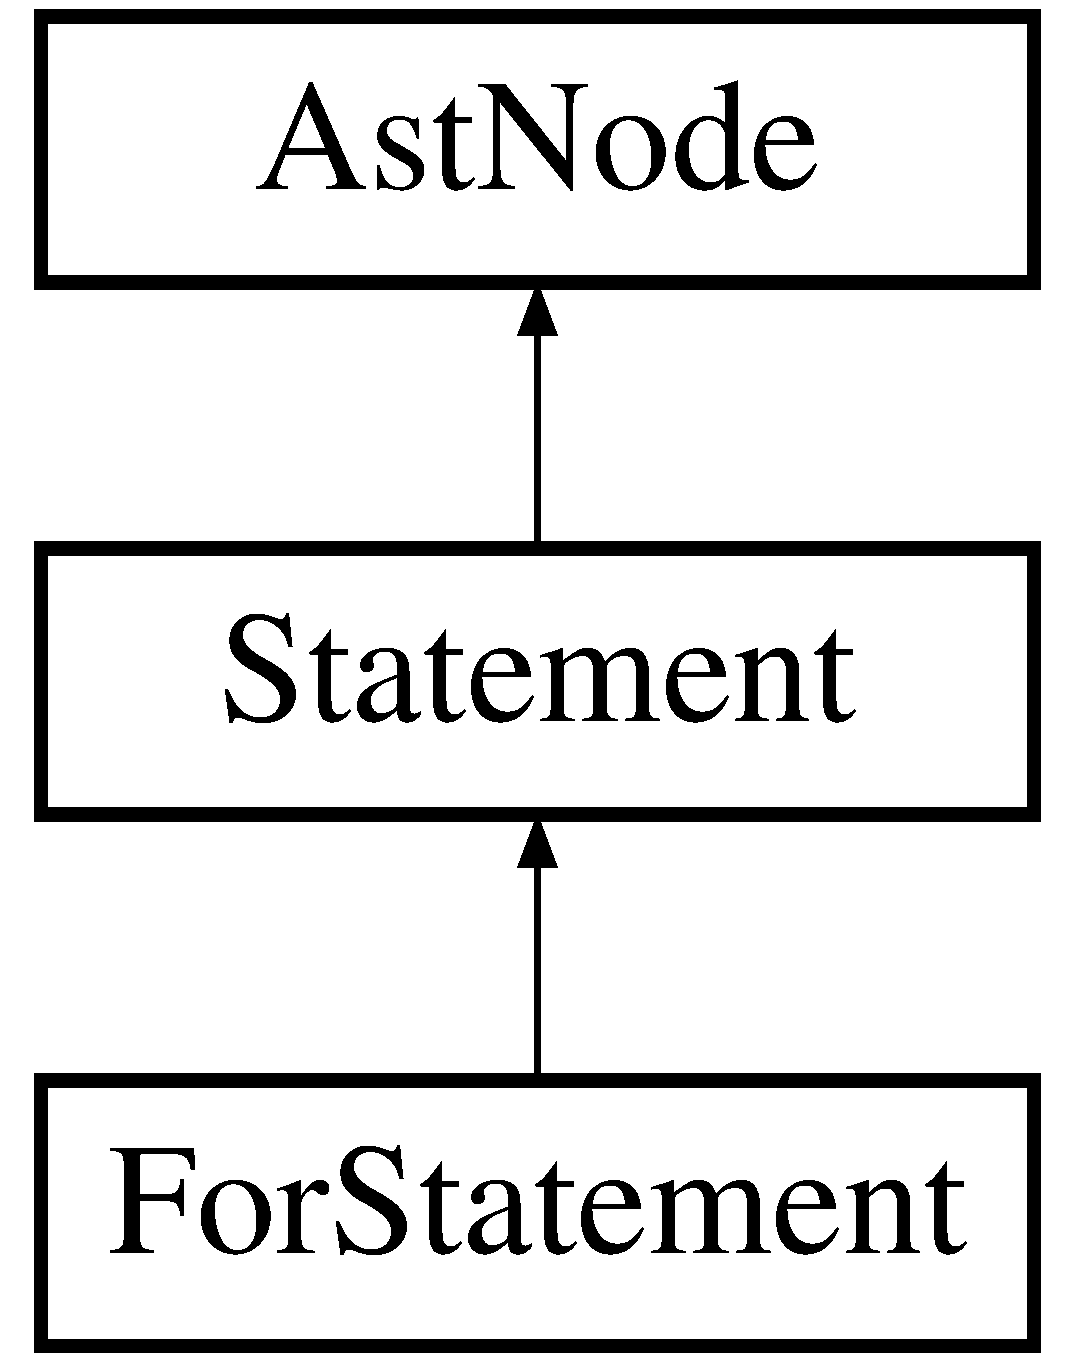
\includegraphics[height=3cm]{classForStatement}
\end{center}
\end{figure}
\subsection*{Public Member Functions}
\begin{DoxyCompactItemize}
\item 
\hyperlink{classForStatement_a34f22456bd665a1d358716e7e71a2eb1}{ForStatement} (int lno, const char $\ast$n, \hyperlink{classExpression}{Expression} $\ast$i, \hyperlink{classExpression}{Expression} $\ast$t, \hyperlink{classExpression}{Expression} $\ast$u, \hyperlink{classStatement}{Statement} $\ast$b)
\item 
\hyperlink{classForStatement_a203c223b6af97279d479734239c76604}{ForStatement} (int lno, const char $\ast$n, \hyperlink{classExpression}{Expression} $\ast$x, \hyperlink{classExpression}{Expression} $\ast$i, \hyperlink{classExpression}{Expression} $\ast$t, \hyperlink{classExpression}{Expression} $\ast$u, \hyperlink{classStatement}{Statement} $\ast$b)
\item 
const char $\ast$ \hyperlink{classForStatement_a15ffa4871bab8d925468d7171e621562}{getLHSName} ()
\item 
ENTRY $\ast$ \hyperlink{classForStatement_a42b0ef907ad4181b001392c7cb496cdf}{getEntry} ()
\item 
void \hyperlink{classForStatement_a1634064d332150b7a62ac40813776f84}{setEntry} (ENTRY $\ast$e)
\item 
\hyperlink{classExpression}{Expression} $\ast$ \hyperlink{classForStatement_a69d2324b4aa27a7bb286e5dfcbebe2bf}{getIndex} ()
\item 
\hyperlink{classExpression}{Expression} $\ast$ \hyperlink{classForStatement_a114c3ab74b627e7dcf33868864596d97}{getInit} ()
\item 
\hyperlink{classExpression}{Expression} $\ast$ \hyperlink{classForStatement_a7ecbeae3c4766ceb9510e02740284467}{getTerm} ()
\item 
\hyperlink{classExpression}{Expression} $\ast$ \hyperlink{classForStatement_a81f61002e628cff42005f4dce5c477f2}{getUpd} ()
\item 
\hyperlink{classStatement}{Statement} $\ast$ \hyperlink{classForStatement_ae52531005fd0fd8cb5e19bba89679548}{getBodyStatement} ()
\item 
void \hyperlink{classForStatement_af81e95d20aa9fe2e84cf1611845653bb}{setBodyStatement} (\hyperlink{classStatement}{Statement} $\ast$b)
\item 
void \hyperlink{classForStatement_a8d31a952806bc123a2f6227d4aa17f2f}{accept} (\hyperlink{classAstVisitor}{AstVisitor} $\ast$aVisitor)
\end{DoxyCompactItemize}


\subsection{Detailed Description}
This class represents a TinyJava FOR statement. The syntax of the for statement is either
\begin{DoxyItemize}
\item FOR '(' IDENT '=' initExpression ';' termExpression ';' updateExpression ')' statement
\end{DoxyItemize}

or


\begin{DoxyItemize}
\item FOR '(' IDENT '\mbox{[}' indexExpression '\mbox{]}' '=' initExpression ';' termExpression ';' updateExpression ')' statement
\end{DoxyItemize}

A for statement is represented by:
\begin{DoxyItemize}
\item identifier on the left-\/hand side of the initialization expression
\item an index \hyperlink{classExpression}{Expression}, if the left hand side is an array element
\item an initialization \hyperlink{classExpression}{Expression}
\item a termination \hyperlink{classExpression}{Expression}
\item an update \hyperlink{classExpression}{Expression}, and
\item a for statement body, that is another \hyperlink{classStatement}{Statement}. A symbol table ENTRY pointer may be provided, as well.
\end{DoxyItemize}

ENTRY should be defined as a macro, and its value should be a class, which is the root of the symbol table entry hierarchy. Its default value is Entry. The macro should be defined at the beginning of the header file Ast.h. 

\subsection{Constructor \& Destructor Documentation}
\hypertarget{classForStatement_a34f22456bd665a1d358716e7e71a2eb1}{
\index{ForStatement@{ForStatement}!ForStatement@{ForStatement}}
\index{ForStatement@{ForStatement}!ForStatement@{ForStatement}}
\subsubsection[{ForStatement}]{\setlength{\rightskip}{0pt plus 5cm}ForStatement::ForStatement (int {\em lno}, \/  const char $\ast$ {\em n}, \/  {\bf Expression} $\ast$ {\em i}, \/  {\bf Expression} $\ast$ {\em t}, \/  {\bf Expression} $\ast$ {\em u}, \/  {\bf Statement} $\ast$ {\em b})}}
\label{classForStatement_a34f22456bd665a1d358716e7e71a2eb1}
Create a new \hyperlink{classForStatement}{ForStatement} object.


\begin{DoxyParams}{Parameters}
\item[{\em lno}]a source code line number with the for statement (should be the beginning of the for statement) \item[{\em n}]a string representing the name on the left-\/hand side of the initialization expression \item[{\em i}]a pointer to an \hyperlink{classExpression}{Expression} representing the initialization expression \item[{\em t}]a pointer to an \hyperlink{classExpression}{Expression} representing the termination expression \item[{\em u}]a pointer to an \hyperlink{classExpression}{Expression} representing the update expression \item[{\em b}]a pointer to a \hyperlink{classStatement}{Statement} representing the for statement body \end{DoxyParams}

\begin{DoxyExceptions}{Exceptions}
\item[{\em \hyperlink{classAstException}{AstException}}]if either the n, i, t, u, or b argument is NULL \end{DoxyExceptions}
\hypertarget{classForStatement_a203c223b6af97279d479734239c76604}{
\index{ForStatement@{ForStatement}!ForStatement@{ForStatement}}
\index{ForStatement@{ForStatement}!ForStatement@{ForStatement}}
\subsubsection[{ForStatement}]{\setlength{\rightskip}{0pt plus 5cm}ForStatement::ForStatement (int {\em lno}, \/  const char $\ast$ {\em n}, \/  {\bf Expression} $\ast$ {\em x}, \/  {\bf Expression} $\ast$ {\em i}, \/  {\bf Expression} $\ast$ {\em t}, \/  {\bf Expression} $\ast$ {\em u}, \/  {\bf Statement} $\ast$ {\em b})}}
\label{classForStatement_a203c223b6af97279d479734239c76604}
Create a new \hyperlink{classForStatement}{ForStatement} object.


\begin{DoxyParams}{Parameters}
\item[{\em lno}]a source code line number with the for statement (should be the beginning of the for statement) \item[{\em n}]a string representing the name on the left-\/hand side of the initialization expression \item[{\em x}]a pointer to an \hyperlink{classExpression}{Expression} representing the index (subscript) expression, if the left hand side is an array elemnt \item[{\em i}]a pointer to an \hyperlink{classExpression}{Expression} representing the initialization expression \item[{\em t}]a pointer to an \hyperlink{classExpression}{Expression} representing the termination expression \item[{\em u}]a pointer to an \hyperlink{classExpression}{Expression} representing the update expression \item[{\em b}]a pointer to a \hyperlink{classStatement}{Statement} representing the for statement body \end{DoxyParams}

\begin{DoxyExceptions}{Exceptions}
\item[{\em \hyperlink{classAstException}{AstException}}]if either the n, x, i, t, u, or b argument is NULL \end{DoxyExceptions}


\subsection{Member Function Documentation}
\hypertarget{classForStatement_a8d31a952806bc123a2f6227d4aa17f2f}{
\index{ForStatement@{ForStatement}!accept@{accept}}
\index{accept@{accept}!ForStatement@{ForStatement}}
\subsubsection[{accept}]{\setlength{\rightskip}{0pt plus 5cm}void ForStatement::accept ({\bf AstVisitor} $\ast$ {\em aVisitor})\hspace{0.3cm}{\ttfamily  \mbox{[}inline, virtual\mbox{]}}}}
\label{classForStatement_a8d31a952806bc123a2f6227d4aa17f2f}
Accept a visitor to this node. 
\begin{DoxyParams}{Parameters}
\item[{\em aVisitor}]is a visitor object of type \hyperlink{classAstVisitor}{AstVisitor}. \end{DoxyParams}


Implements \hyperlink{classAstNode_a67b2d6ce1262da2954fb4db255759fb3}{AstNode}.\hypertarget{classForStatement_ae52531005fd0fd8cb5e19bba89679548}{
\index{ForStatement@{ForStatement}!getBodyStatement@{getBodyStatement}}
\index{getBodyStatement@{getBodyStatement}!ForStatement@{ForStatement}}
\subsubsection[{getBodyStatement}]{\setlength{\rightskip}{0pt plus 5cm}{\bf Statement}$\ast$ ForStatement::getBodyStatement ()\hspace{0.3cm}{\ttfamily  \mbox{[}inline\mbox{]}}}}
\label{classForStatement_ae52531005fd0fd8cb5e19bba89679548}
Return the body of this for statement

\begin{DoxyReturn}{Returns}
pointer to a \hyperlink{classStatement}{Statement} representing the body of the for statement 
\end{DoxyReturn}
\hypertarget{classForStatement_a42b0ef907ad4181b001392c7cb496cdf}{
\index{ForStatement@{ForStatement}!getEntry@{getEntry}}
\index{getEntry@{getEntry}!ForStatement@{ForStatement}}
\subsubsection[{getEntry}]{\setlength{\rightskip}{0pt plus 5cm}ENTRY$\ast$ ForStatement::getEntry ()\hspace{0.3cm}{\ttfamily  \mbox{[}inline\mbox{]}}}}
\label{classForStatement_a42b0ef907ad4181b001392c7cb496cdf}
Return a pointer to the symbol table entry representing the left-\/hand side of the initialization expression.

\begin{DoxyReturn}{Returns}
ENTRY pointer to the symbol table. 
\end{DoxyReturn}
\hypertarget{classForStatement_a69d2324b4aa27a7bb286e5dfcbebe2bf}{
\index{ForStatement@{ForStatement}!getIndex@{getIndex}}
\index{getIndex@{getIndex}!ForStatement@{ForStatement}}
\subsubsection[{getIndex}]{\setlength{\rightskip}{0pt plus 5cm}{\bf Expression}$\ast$ ForStatement::getIndex ()\hspace{0.3cm}{\ttfamily  \mbox{[}inline\mbox{]}}}}
\label{classForStatement_a69d2324b4aa27a7bb286e5dfcbebe2bf}
Return the index (subscript) \hyperlink{classExpression}{Expression}, if the left hand side is an array element.

\begin{DoxyReturn}{Returns}
pointer to an \hyperlink{classExpression}{Expression} representing the array index (subscript). 
\end{DoxyReturn}
\hypertarget{classForStatement_a114c3ab74b627e7dcf33868864596d97}{
\index{ForStatement@{ForStatement}!getInit@{getInit}}
\index{getInit@{getInit}!ForStatement@{ForStatement}}
\subsubsection[{getInit}]{\setlength{\rightskip}{0pt plus 5cm}{\bf Expression}$\ast$ ForStatement::getInit ()\hspace{0.3cm}{\ttfamily  \mbox{[}inline\mbox{]}}}}
\label{classForStatement_a114c3ab74b627e7dcf33868864596d97}
Return the initialization \hyperlink{classExpression}{Expression} of this for statement

\begin{DoxyReturn}{Returns}
pointer to an \hyperlink{classExpression}{Expression} epresenting the initialization \hyperlink{classExpression}{Expression} 
\end{DoxyReturn}
\hypertarget{classForStatement_a15ffa4871bab8d925468d7171e621562}{
\index{ForStatement@{ForStatement}!getLHSName@{getLHSName}}
\index{getLHSName@{getLHSName}!ForStatement@{ForStatement}}
\subsubsection[{getLHSName}]{\setlength{\rightskip}{0pt plus 5cm}const char$\ast$ ForStatement::getLHSName ()\hspace{0.3cm}{\ttfamily  \mbox{[}inline\mbox{]}}}}
\label{classForStatement_a15ffa4871bab8d925468d7171e621562}
Return the identifier (variable, field, or parameter) on the left hand side of this assignment statement.

\begin{DoxyReturn}{Returns}
a string representing the left-\/hand side identifier. 
\end{DoxyReturn}
\hypertarget{classForStatement_a7ecbeae3c4766ceb9510e02740284467}{
\index{ForStatement@{ForStatement}!getTerm@{getTerm}}
\index{getTerm@{getTerm}!ForStatement@{ForStatement}}
\subsubsection[{getTerm}]{\setlength{\rightskip}{0pt plus 5cm}{\bf Expression}$\ast$ ForStatement::getTerm ()\hspace{0.3cm}{\ttfamily  \mbox{[}inline\mbox{]}}}}
\label{classForStatement_a7ecbeae3c4766ceb9510e02740284467}
Return the termination \hyperlink{classExpression}{Expression} of this for statement

\begin{DoxyReturn}{Returns}
pointer to an \hyperlink{classExpression}{Expression} epresenting the termination \hyperlink{classExpression}{Expression} 
\end{DoxyReturn}
\hypertarget{classForStatement_a81f61002e628cff42005f4dce5c477f2}{
\index{ForStatement@{ForStatement}!getUpd@{getUpd}}
\index{getUpd@{getUpd}!ForStatement@{ForStatement}}
\subsubsection[{getUpd}]{\setlength{\rightskip}{0pt plus 5cm}{\bf Expression}$\ast$ ForStatement::getUpd ()\hspace{0.3cm}{\ttfamily  \mbox{[}inline\mbox{]}}}}
\label{classForStatement_a81f61002e628cff42005f4dce5c477f2}
Return the update \hyperlink{classExpression}{Expression} of this for statement

\begin{DoxyReturn}{Returns}
pointer to an \hyperlink{classExpression}{Expression} epresenting the update \hyperlink{classExpression}{Expression} 
\end{DoxyReturn}
\hypertarget{classForStatement_af81e95d20aa9fe2e84cf1611845653bb}{
\index{ForStatement@{ForStatement}!setBodyStatement@{setBodyStatement}}
\index{setBodyStatement@{setBodyStatement}!ForStatement@{ForStatement}}
\subsubsection[{setBodyStatement}]{\setlength{\rightskip}{0pt plus 5cm}void ForStatement::setBodyStatement ({\bf Statement} $\ast$ {\em b})\hspace{0.3cm}{\ttfamily  \mbox{[}inline\mbox{]}}}}
\label{classForStatement_af81e95d20aa9fe2e84cf1611845653bb}
Set the the body of this for statement


\begin{DoxyParams}{Parameters}
\item[{\em b}]a pointer to a \hyperlink{classStatement}{Statement} representing the body of the for statement \end{DoxyParams}

\begin{DoxyExceptions}{Exceptions}
\item[{\em \hyperlink{classAstException}{AstException}}]if the argument is NULL \end{DoxyExceptions}
\hypertarget{classForStatement_a1634064d332150b7a62ac40813776f84}{
\index{ForStatement@{ForStatement}!setEntry@{setEntry}}
\index{setEntry@{setEntry}!ForStatement@{ForStatement}}
\subsubsection[{setEntry}]{\setlength{\rightskip}{0pt plus 5cm}void ForStatement::setEntry (ENTRY $\ast$ {\em e})\hspace{0.3cm}{\ttfamily  \mbox{[}inline\mbox{]}}}}
\label{classForStatement_a1634064d332150b7a62ac40813776f84}
Set the symbol table ENTRY representing the left-\/hand side of the initialization expression.


\begin{DoxyParams}{Parameters}
\item[{\em e}]an ENTRY pointer to the new symbol table ENTRY \end{DoxyParams}


The documentation for this class was generated from the following files:\begin{DoxyCompactItemize}
\item 
ForStmt.h\item 
ForStmt.cpp\end{DoxyCompactItemize}

\hypertarget{classIfStatement}{
\section{IfStatement Class Reference}
\label{classIfStatement}\index{IfStatement@{IfStatement}}
}


This class represents a TinyJava IF statement.  


{\ttfamily \#include $<$IfStmt.h$>$}Inheritance diagram for IfStatement::\begin{figure}[H]
\begin{center}
\leavevmode
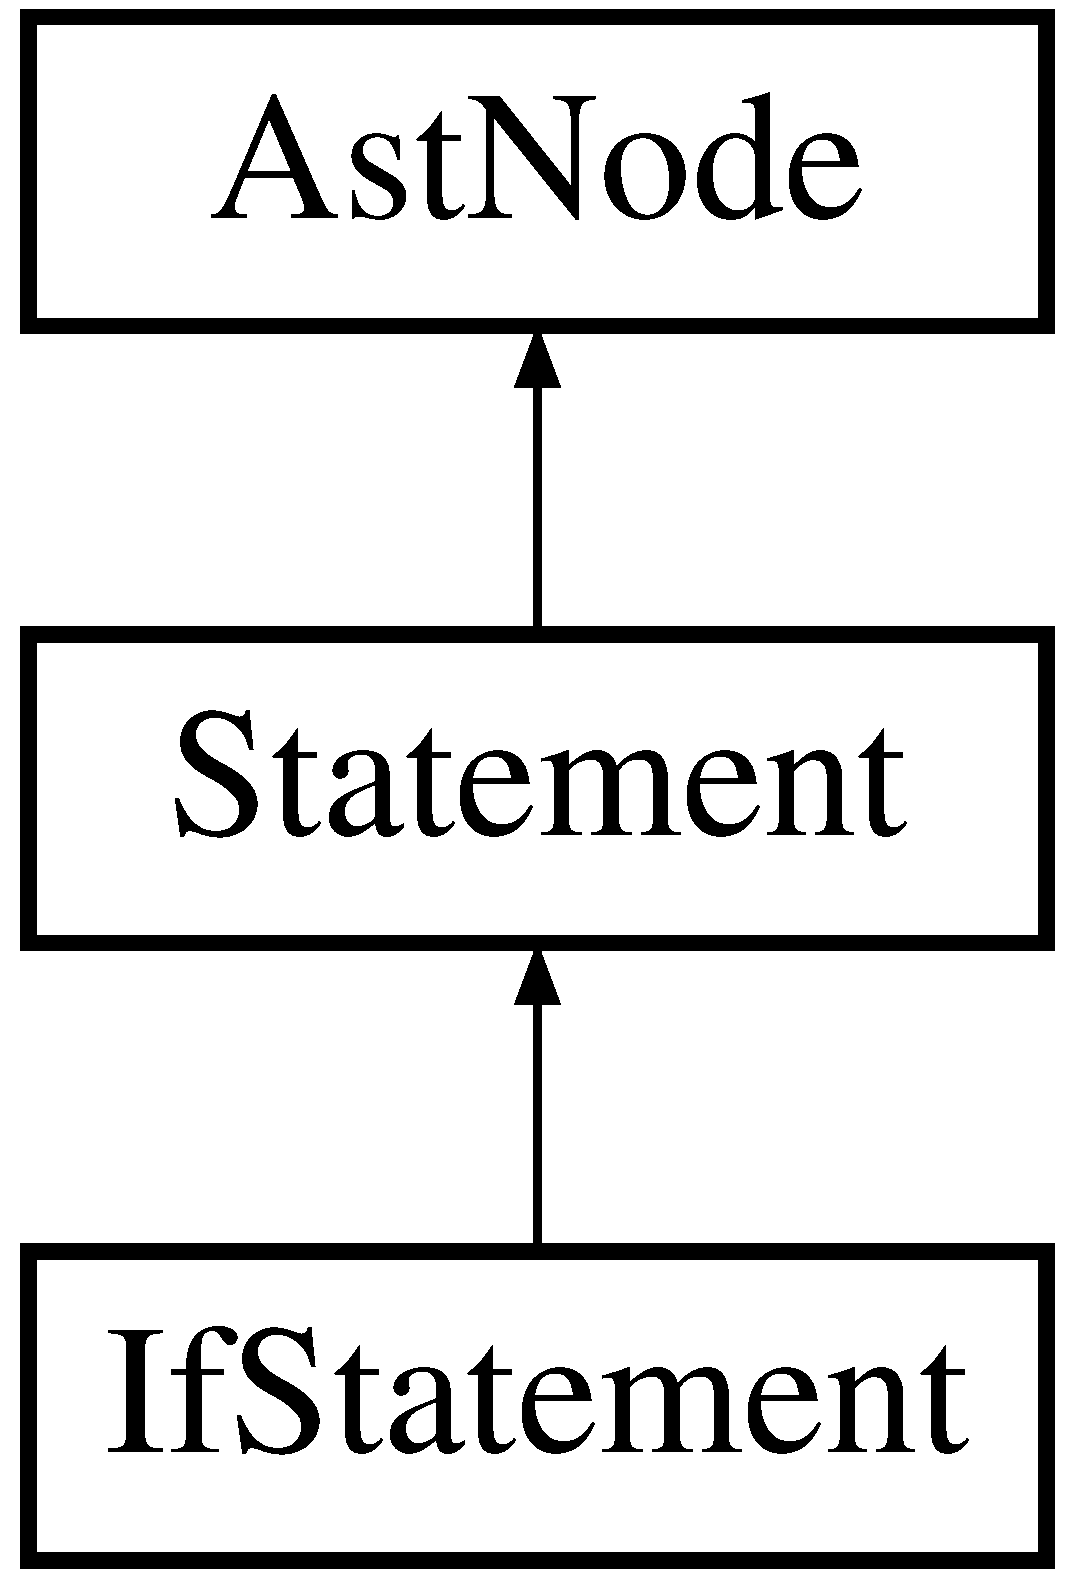
\includegraphics[height=3cm]{classIfStatement}
\end{center}
\end{figure}
\subsection*{Public Member Functions}
\begin{DoxyCompactItemize}
\item 
\hyperlink{classIfStatement_af99bd97270bb7f31932e9ccd3c85d9d3}{IfStatement} (int lno, \hyperlink{classExpression}{Expression} $\ast$e, \hyperlink{classStatement}{Statement} $\ast$ts, \hyperlink{classStatement}{Statement} $\ast$es)
\item 
\hyperlink{classExpression}{Expression} $\ast$ \hyperlink{classIfStatement_aa9a02bb22bf3f74c87fb979aa889d6b6}{getExpression} ()
\item 
\hyperlink{classStatement}{Statement} $\ast$ \hyperlink{classIfStatement_a77b917ab2b788e992f60ab5a1e56678b}{getThenStatement} ()
\item 
\hyperlink{classStatement}{Statement} $\ast$ \hyperlink{classIfStatement_a79a1c2c1a1d824c0160cdef2b9f87478}{getElseStatement} ()
\item 
void \hyperlink{classIfStatement_ab4c2cd2f1c924951d782493281d15249}{accept} (\hyperlink{classAstVisitor}{AstVisitor} $\ast$aVisitor)
\end{DoxyCompactItemize}


\subsection{Detailed Description}
This class represents a TinyJava IF statement. An if statement is represented by:
\begin{DoxyItemize}
\item a control \hyperlink{classExpression}{Expression} representation
\item a then \hyperlink{classStatement}{Statement} representation
\item an else \hyperlink{classStatement}{Statement} representation, which may be NULL 
\end{DoxyItemize}

\subsection{Constructor \& Destructor Documentation}
\hypertarget{classIfStatement_af99bd97270bb7f31932e9ccd3c85d9d3}{
\index{IfStatement@{IfStatement}!IfStatement@{IfStatement}}
\index{IfStatement@{IfStatement}!IfStatement@{IfStatement}}
\subsubsection[{IfStatement}]{\setlength{\rightskip}{0pt plus 5cm}IfStatement::IfStatement (int {\em lno}, \/  {\bf Expression} $\ast$ {\em e}, \/  {\bf Statement} $\ast$ {\em ts}, \/  {\bf Statement} $\ast$ {\em es})}}
\label{classIfStatement_af99bd97270bb7f31932e9ccd3c85d9d3}
Create a new \hyperlink{classIfStatement}{IfStatement} object


\begin{DoxyParams}{Parameters}
\item[{\em lno}]a source code line number with the if statement (should be the beginning of the if statement) \item[{\em e}]a pointer to the control \hyperlink{classExpression}{Expression} syntax tree \item[{\em ts}]a pointer to the THEN \hyperlink{classStatement}{Statement} syntax tree \item[{\em es}]a pointer to the ELSE \hyperlink{classStatement}{Statement} syntax tree, which may be NULL if the if statement has no ELSE part \end{DoxyParams}

\begin{DoxyExceptions}{Exceptions}
\item[{\em \hyperlink{classAstException}{AstException}}]if either the e or ts argument is NULL \end{DoxyExceptions}


\subsection{Member Function Documentation}
\hypertarget{classIfStatement_ab4c2cd2f1c924951d782493281d15249}{
\index{IfStatement@{IfStatement}!accept@{accept}}
\index{accept@{accept}!IfStatement@{IfStatement}}
\subsubsection[{accept}]{\setlength{\rightskip}{0pt plus 5cm}void IfStatement::accept ({\bf AstVisitor} $\ast$ {\em aVisitor})\hspace{0.3cm}{\ttfamily  \mbox{[}inline, virtual\mbox{]}}}}
\label{classIfStatement_ab4c2cd2f1c924951d782493281d15249}
Accept a visitor to this node. 
\begin{DoxyParams}{Parameters}
\item[{\em aVisitor}]is a visitor object of type \hyperlink{classAstVisitor}{AstVisitor}. \end{DoxyParams}


Implements \hyperlink{classAstNode_a67b2d6ce1262da2954fb4db255759fb3}{AstNode}.\hypertarget{classIfStatement_a79a1c2c1a1d824c0160cdef2b9f87478}{
\index{IfStatement@{IfStatement}!getElseStatement@{getElseStatement}}
\index{getElseStatement@{getElseStatement}!IfStatement@{IfStatement}}
\subsubsection[{getElseStatement}]{\setlength{\rightskip}{0pt plus 5cm}{\bf Statement}$\ast$ IfStatement::getElseStatement ()\hspace{0.3cm}{\ttfamily  \mbox{[}inline\mbox{]}}}}
\label{classIfStatement_a79a1c2c1a1d824c0160cdef2b9f87478}
Return the ELSE statement of this if statement

\begin{DoxyReturn}{Returns}
pointer to a \hyperlink{classStatement}{Statement} representing the ELSE statement 
\end{DoxyReturn}
\hypertarget{classIfStatement_aa9a02bb22bf3f74c87fb979aa889d6b6}{
\index{IfStatement@{IfStatement}!getExpression@{getExpression}}
\index{getExpression@{getExpression}!IfStatement@{IfStatement}}
\subsubsection[{getExpression}]{\setlength{\rightskip}{0pt plus 5cm}{\bf Expression}$\ast$ IfStatement::getExpression ()\hspace{0.3cm}{\ttfamily  \mbox{[}inline\mbox{]}}}}
\label{classIfStatement_aa9a02bb22bf3f74c87fb979aa889d6b6}
Return the control \hyperlink{classExpression}{Expression} of this if statement

\begin{DoxyReturn}{Returns}
pointer to an \hyperlink{classExpression}{Expression} representing the control expression 
\end{DoxyReturn}
\hypertarget{classIfStatement_a77b917ab2b788e992f60ab5a1e56678b}{
\index{IfStatement@{IfStatement}!getThenStatement@{getThenStatement}}
\index{getThenStatement@{getThenStatement}!IfStatement@{IfStatement}}
\subsubsection[{getThenStatement}]{\setlength{\rightskip}{0pt plus 5cm}{\bf Statement}$\ast$ IfStatement::getThenStatement ()\hspace{0.3cm}{\ttfamily  \mbox{[}inline\mbox{]}}}}
\label{classIfStatement_a77b917ab2b788e992f60ab5a1e56678b}
Return the THEN statement of this if statement

\begin{DoxyReturn}{Returns}
pointer to a \hyperlink{classStatement}{Statement} representing the THEN statement 
\end{DoxyReturn}


The documentation for this class was generated from the following files:\begin{DoxyCompactItemize}
\item 
IfStmt.h\item 
IfStmt.cpp\end{DoxyCompactItemize}

\hypertarget{classLiteralExpression}{
\section{LiteralExpression Class Reference}
\label{classLiteralExpression}\index{LiteralExpression@{LiteralExpression}}
}


This class represents a TinyJava literal (smallest expression).  


{\ttfamily \#include $<$LiteralExpression.h$>$}Inheritance diagram for LiteralExpression::\begin{figure}[H]
\begin{center}
\leavevmode
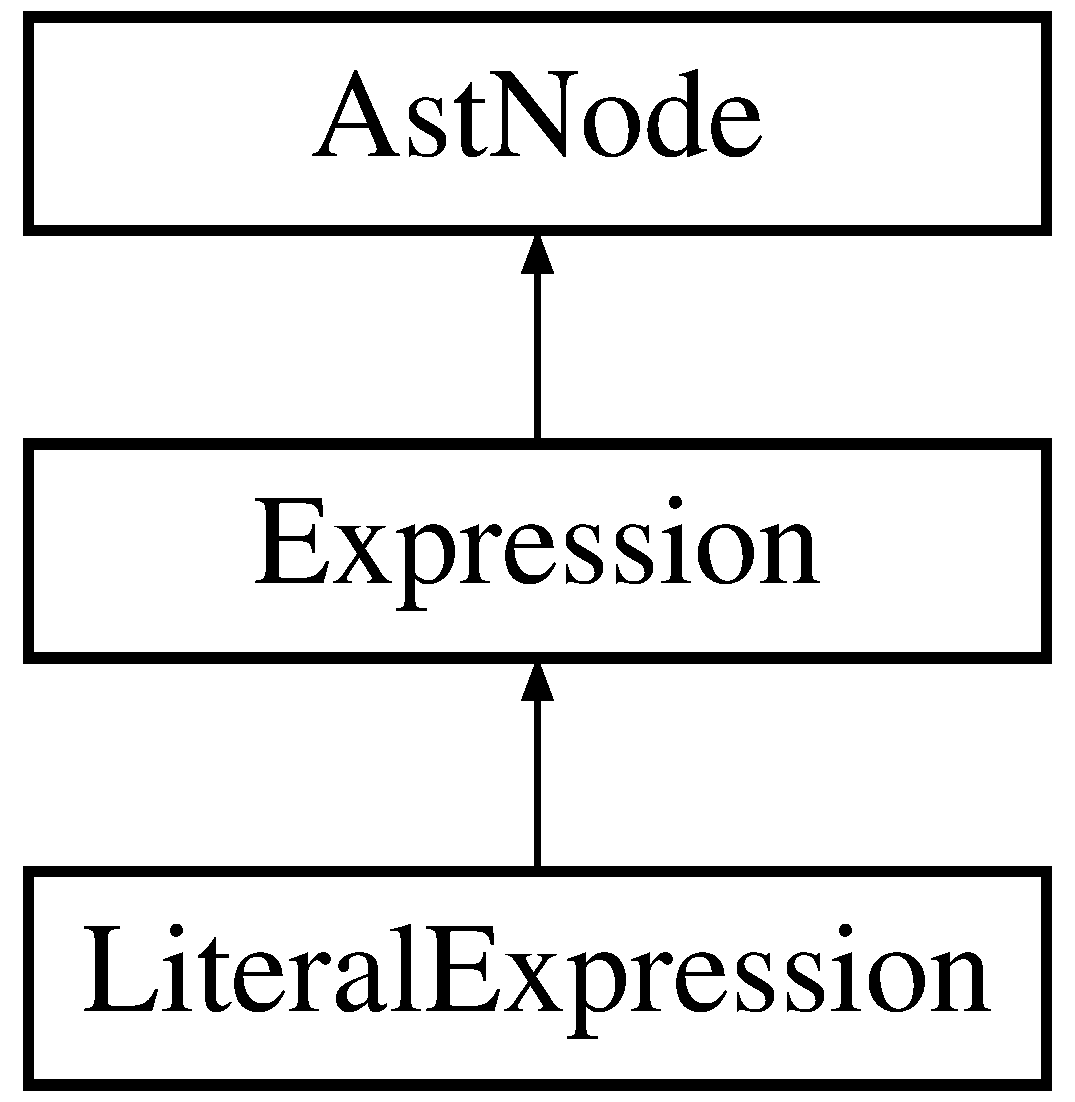
\includegraphics[height=3cm]{classLiteralExpression}
\end{center}
\end{figure}
\subsection*{Public Member Functions}
\begin{DoxyCompactItemize}
\item 
\hyperlink{classLiteralExpression_a4401fd6efc3f6808d28d64a734070df6}{LiteralExpression} (int lno, const char $\ast$lit, int tp)
\item 
const char $\ast$ \hyperlink{classLiteralExpression_a6e8ba5b0d9da137dfe00750cbfe125b3}{getLiteral} ()
\item 
void \hyperlink{classLiteralExpression_a02054e805df96a9d75ea64acc35d15a7}{accept} (\hyperlink{classAstVisitor}{AstVisitor} $\ast$aVisitor)
\end{DoxyCompactItemize}


\subsection{Detailed Description}
This class represents a TinyJava literal (smallest expression). The literal is represented as a string. It is always a leaf in an Abstract Syntax Tree. 

\subsection{Constructor \& Destructor Documentation}
\hypertarget{classLiteralExpression_a4401fd6efc3f6808d28d64a734070df6}{
\index{LiteralExpression@{LiteralExpression}!LiteralExpression@{LiteralExpression}}
\index{LiteralExpression@{LiteralExpression}!LiteralExpression@{LiteralExpression}}
\subsubsection[{LiteralExpression}]{\setlength{\rightskip}{0pt plus 5cm}LiteralExpression::LiteralExpression (int {\em lno}, \/  const char $\ast$ {\em lit}, \/  int {\em tp})\hspace{0.3cm}{\ttfamily  \mbox{[}inline\mbox{]}}}}
\label{classLiteralExpression_a4401fd6efc3f6808d28d64a734070df6}
Create a new \hyperlink{classLiteralExpression}{LiteralExpression} object.


\begin{DoxyParams}{Parameters}
\item[{\em lno}]is a source line number with this literal \item[{\em lit}]a string representing the literal value \item[{\em tp}]an integer representing the type, as defined in the \hyperlink{classAstNode}{AstNode} class \end{DoxyParams}

\begin{DoxyExceptions}{Exceptions}
\item[{\em \hyperlink{classAstException}{AstException}}]if the lit argument is NULL \end{DoxyExceptions}


\subsection{Member Function Documentation}
\hypertarget{classLiteralExpression_a02054e805df96a9d75ea64acc35d15a7}{
\index{LiteralExpression@{LiteralExpression}!accept@{accept}}
\index{accept@{accept}!LiteralExpression@{LiteralExpression}}
\subsubsection[{accept}]{\setlength{\rightskip}{0pt plus 5cm}void LiteralExpression::accept ({\bf AstVisitor} $\ast$ {\em aVisitor})\hspace{0.3cm}{\ttfamily  \mbox{[}inline, virtual\mbox{]}}}}
\label{classLiteralExpression_a02054e805df96a9d75ea64acc35d15a7}
Accept a visitor to this node. 
\begin{DoxyParams}{Parameters}
\item[{\em aVisitor}]is a visitor object of type \hyperlink{classAstVisitor}{AstVisitor}. \end{DoxyParams}


Implements \hyperlink{classAstNode_a67b2d6ce1262da2954fb4db255759fb3}{AstNode}.\hypertarget{classLiteralExpression_a6e8ba5b0d9da137dfe00750cbfe125b3}{
\index{LiteralExpression@{LiteralExpression}!getLiteral@{getLiteral}}
\index{getLiteral@{getLiteral}!LiteralExpression@{LiteralExpression}}
\subsubsection[{getLiteral}]{\setlength{\rightskip}{0pt plus 5cm}const char$\ast$ LiteralExpression::getLiteral ()\hspace{0.3cm}{\ttfamily  \mbox{[}inline\mbox{]}}}}
\label{classLiteralExpression_a6e8ba5b0d9da137dfe00750cbfe125b3}
Return the literal value.

\begin{DoxyReturn}{Returns}
a string representing the literal value 
\end{DoxyReturn}


The documentation for this class was generated from the following file:\begin{DoxyCompactItemize}
\item 
LiteralExpression.h\end{DoxyCompactItemize}

\hypertarget{classMethodCallExpression}{
\section{MethodCallExpression Class Reference}
\label{classMethodCallExpression}\index{MethodCallExpression@{MethodCallExpression}}
}


This class represents a TinyJava method call expression.  


{\ttfamily \#include $<$MethodCallExpression.h$>$}Inheritance diagram for MethodCallExpression::\begin{figure}[H]
\begin{center}
\leavevmode
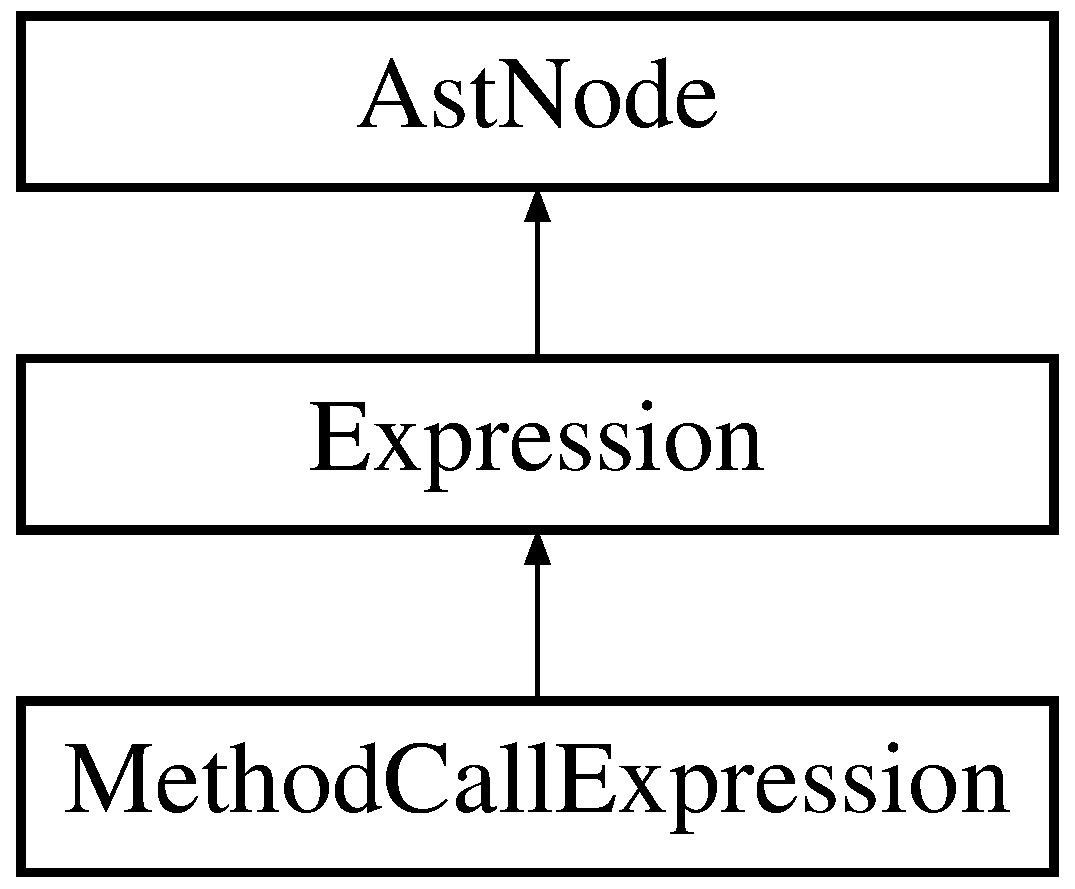
\includegraphics[height=3cm]{classMethodCallExpression}
\end{center}
\end{figure}
\subsection*{Public Member Functions}
\begin{DoxyCompactItemize}
\item 
\hyperlink{classMethodCallExpression_a5019b48097b4bcddd2016e19e7aa9b21}{MethodCallExpression} (int lno, const char $\ast$className, const char $\ast$methodName, std::vector$<$ \hyperlink{classExpression}{Expression} $\ast$ $>$ $\ast$args)
\item 
const char $\ast$ \hyperlink{classMethodCallExpression_aac842be4123a65f75e09dad4369fcdb2}{getClassName} ()
\item 
const char $\ast$ \hyperlink{classMethodCallExpression_a53338c550e4f939f8c263f08a52ec8f5}{getMethodName} ()
\item 
ENTRY $\ast$ \hyperlink{classMethodCallExpression_acba6b59d3a951124c09bc8222dea1b82}{getEntry} ()
\item 
void \hyperlink{classMethodCallExpression_a573fa44f50e5c3c55e0801d726ccf594}{setEntry} (ENTRY $\ast$e)
\item 
int \hyperlink{classMethodCallExpression_ac827bda72aa7edd546dc70ba7e4dea7a}{getNoArguments} ()
\item 
\hyperlink{classExpression}{Expression} $\ast$ \hyperlink{classMethodCallExpression_a8fdb332750c263169f163cd15bf2181c}{getArgument} (int pos)
\item 
std::vector$<$ \hyperlink{classExpression}{Expression} $\ast$ $>$ $\ast$ \hyperlink{classMethodCallExpression_ac8d64b39cf5cce5ff7baaef80e9c8911}{getArguments} ()
\item 
void \hyperlink{classMethodCallExpression_a31c2b10a2914b5a71d16feab9bb96d34}{setArguments} (std::vector$<$ \hyperlink{classExpression}{Expression} $\ast$ $>$ $\ast$args)
\item 
void \hyperlink{classMethodCallExpression_a40f6c0c6861cc3ea50253a47a7ec6879}{addArgument} (\hyperlink{classExpression}{Expression} $\ast$argument)
\item 
void \hyperlink{classMethodCallExpression_a1930d4df840960e60304da85acc70b63}{prependArgument} (\hyperlink{classExpression}{Expression} $\ast$argument)
\item 
void \hyperlink{classMethodCallExpression_a306fe23511d0d35c003a6256816ccea6}{accept} (\hyperlink{classAstVisitor}{AstVisitor} $\ast$aVisitor)
\end{DoxyCompactItemize}


\subsection{Detailed Description}
This class represents a TinyJava method call expression. A nethod call expression is represented by:
\begin{DoxyItemize}
\item class name, if the referenced method is a static method in a different class
\item method name; a pointer to the symbol table ENTRY for the name may also be included.
\item call arguments
\end{DoxyItemize}

ENTRY should be defined as a macro, and its value should be a class, which is the root of the symbol table entry hierarchy. Its default value is Entry. The macro should be defined at the beginning of the header file Ast.h. 

\subsection{Constructor \& Destructor Documentation}
\hypertarget{classMethodCallExpression_a5019b48097b4bcddd2016e19e7aa9b21}{
\index{MethodCallExpression@{MethodCallExpression}!MethodCallExpression@{MethodCallExpression}}
\index{MethodCallExpression@{MethodCallExpression}!MethodCallExpression@{MethodCallExpression}}
\subsubsection[{MethodCallExpression}]{\setlength{\rightskip}{0pt plus 5cm}MethodCallExpression::MethodCallExpression (int {\em lno}, \/  const char $\ast$ {\em className}, \/  const char $\ast$ {\em methodName}, \/  std::vector$<$ {\bf Expression} $\ast$ $>$ $\ast$ {\em args})}}
\label{classMethodCallExpression_a5019b48097b4bcddd2016e19e7aa9b21}
Create a new \hyperlink{classMethodCallExpression}{MethodCallExpression} object. The default type of this \hyperlink{classExpression}{Expression} is set to \hyperlink{classAstNode_a8568313f5d280773a446280c94d382f8}{AstNode::TINT}.


\begin{DoxyParams}{Parameters}
\item[{\em lno}]a source line number with this method call expression \item[{\em className}]a string representing the class name with the method (if thie is a qualified name) \item[{\em methodName}]a string representing the method name \item[{\em args}]a std::vector of \hyperlink{classExpression}{Expression} pointers, each representing an argument expression \end{DoxyParams}

\begin{DoxyExceptions}{Exceptions}
\item[{\em \hyperlink{classAstException}{AstException}}]if the methodName is NULL \end{DoxyExceptions}


\subsection{Member Function Documentation}
\hypertarget{classMethodCallExpression_a306fe23511d0d35c003a6256816ccea6}{
\index{MethodCallExpression@{MethodCallExpression}!accept@{accept}}
\index{accept@{accept}!MethodCallExpression@{MethodCallExpression}}
\subsubsection[{accept}]{\setlength{\rightskip}{0pt plus 5cm}void MethodCallExpression::accept ({\bf AstVisitor} $\ast$ {\em aVisitor})\hspace{0.3cm}{\ttfamily  \mbox{[}inline, virtual\mbox{]}}}}
\label{classMethodCallExpression_a306fe23511d0d35c003a6256816ccea6}
Accept a visitor to this node. 
\begin{DoxyParams}{Parameters}
\item[{\em aVisitor}]is a visitor object of type \hyperlink{classAstVisitor}{AstVisitor}. \end{DoxyParams}


Implements \hyperlink{classAstNode_a67b2d6ce1262da2954fb4db255759fb3}{AstNode}.\hypertarget{classMethodCallExpression_a40f6c0c6861cc3ea50253a47a7ec6879}{
\index{MethodCallExpression@{MethodCallExpression}!addArgument@{addArgument}}
\index{addArgument@{addArgument}!MethodCallExpression@{MethodCallExpression}}
\subsubsection[{addArgument}]{\setlength{\rightskip}{0pt plus 5cm}void MethodCallExpression::addArgument ({\bf Expression} $\ast$ {\em argument})}}
\label{classMethodCallExpression_a40f6c0c6861cc3ea50253a47a7ec6879}
Add anther argument to this \hyperlink{classMethodCallExpression}{MethodCallExpression}. The new argument will be the last argumnet.


\begin{DoxyParams}{Parameters}
\item[{\em argument}]an \hyperlink{classExpression}{Expression} pointer representing an argument expression \end{DoxyParams}

\begin{DoxyExceptions}{Exceptions}
\item[{\em \hyperlink{classAstException}{AstException}}]if the argument is NULL \end{DoxyExceptions}
\hypertarget{classMethodCallExpression_a8fdb332750c263169f163cd15bf2181c}{
\index{MethodCallExpression@{MethodCallExpression}!getArgument@{getArgument}}
\index{getArgument@{getArgument}!MethodCallExpression@{MethodCallExpression}}
\subsubsection[{getArgument}]{\setlength{\rightskip}{0pt plus 5cm}{\bf Expression}$\ast$ MethodCallExpression::getArgument (int {\em pos})\hspace{0.3cm}{\ttfamily  \mbox{[}inline\mbox{]}}}}
\label{classMethodCallExpression_a8fdb332750c263169f163cd15bf2181c}
Return the specific argument \hyperlink{classExpression}{Expression}


\begin{DoxyParams}{Parameters}
\item[{\em pos}]the argument position; the first argument is at position 0 \end{DoxyParams}
\begin{DoxyReturn}{Returns}
a pointer to the \hyperlink{classExpression}{Expression} representing the requested argument of this method call 
\end{DoxyReturn}

\begin{DoxyExceptions}{Exceptions}
\item[{\em \hyperlink{classAstException}{AstException}}]if the requested argument does not exist, i.e. if the method call has no arguments, or if the pos value is outside of the argument number range \end{DoxyExceptions}
\hypertarget{classMethodCallExpression_ac8d64b39cf5cce5ff7baaef80e9c8911}{
\index{MethodCallExpression@{MethodCallExpression}!getArguments@{getArguments}}
\index{getArguments@{getArguments}!MethodCallExpression@{MethodCallExpression}}
\subsubsection[{getArguments}]{\setlength{\rightskip}{0pt plus 5cm}std::vector$<${\bf Expression} $\ast$$>$$\ast$ MethodCallExpression::getArguments ()\hspace{0.3cm}{\ttfamily  \mbox{[}inline\mbox{]}}}}
\label{classMethodCallExpression_ac8d64b39cf5cce5ff7baaef80e9c8911}
Return all arguments of this \hyperlink{classMethodCallExpression}{MethodCallExpression}

\begin{DoxyReturn}{Returns}
a pointer to a std::vector of \hyperlink{classExpression}{Expression} pointers, each representing an argument expression 
\end{DoxyReturn}
\hypertarget{classMethodCallExpression_aac842be4123a65f75e09dad4369fcdb2}{
\index{MethodCallExpression@{MethodCallExpression}!getClassName@{getClassName}}
\index{getClassName@{getClassName}!MethodCallExpression@{MethodCallExpression}}
\subsubsection[{getClassName}]{\setlength{\rightskip}{0pt plus 5cm}const char$\ast$ MethodCallExpression::getClassName ()\hspace{0.3cm}{\ttfamily  \mbox{[}inline\mbox{]}}}}
\label{classMethodCallExpression_aac842be4123a65f75e09dad4369fcdb2}
Return the class name of this method call (if a qualified name)

\begin{DoxyReturn}{Returns}
a string representing the class name 
\end{DoxyReturn}
\hypertarget{classMethodCallExpression_acba6b59d3a951124c09bc8222dea1b82}{
\index{MethodCallExpression@{MethodCallExpression}!getEntry@{getEntry}}
\index{getEntry@{getEntry}!MethodCallExpression@{MethodCallExpression}}
\subsubsection[{getEntry}]{\setlength{\rightskip}{0pt plus 5cm}ENTRY$\ast$ MethodCallExpression::getEntry ()\hspace{0.3cm}{\ttfamily  \mbox{[}inline\mbox{]}}}}
\label{classMethodCallExpression_acba6b59d3a951124c09bc8222dea1b82}
Return the symbol table entry for this method

\begin{DoxyReturn}{Returns}
a pointer to the symbol table entry representing the called method 
\end{DoxyReturn}
\hypertarget{classMethodCallExpression_a53338c550e4f939f8c263f08a52ec8f5}{
\index{MethodCallExpression@{MethodCallExpression}!getMethodName@{getMethodName}}
\index{getMethodName@{getMethodName}!MethodCallExpression@{MethodCallExpression}}
\subsubsection[{getMethodName}]{\setlength{\rightskip}{0pt plus 5cm}const char$\ast$ MethodCallExpression::getMethodName ()\hspace{0.3cm}{\ttfamily  \mbox{[}inline\mbox{]}}}}
\label{classMethodCallExpression_a53338c550e4f939f8c263f08a52ec8f5}
Return the method name of this method call

\begin{DoxyReturn}{Returns}
a string representing the method name 
\end{DoxyReturn}
\hypertarget{classMethodCallExpression_ac827bda72aa7edd546dc70ba7e4dea7a}{
\index{MethodCallExpression@{MethodCallExpression}!getNoArguments@{getNoArguments}}
\index{getNoArguments@{getNoArguments}!MethodCallExpression@{MethodCallExpression}}
\subsubsection[{getNoArguments}]{\setlength{\rightskip}{0pt plus 5cm}int MethodCallExpression::getNoArguments ()\hspace{0.3cm}{\ttfamily  \mbox{[}inline\mbox{]}}}}
\label{classMethodCallExpression_ac827bda72aa7edd546dc70ba7e4dea7a}
Return the numbed of arguments in thie method call

\begin{DoxyReturn}{Returns}
the numbed of arguments in thie method call 
\end{DoxyReturn}
\hypertarget{classMethodCallExpression_a1930d4df840960e60304da85acc70b63}{
\index{MethodCallExpression@{MethodCallExpression}!prependArgument@{prependArgument}}
\index{prependArgument@{prependArgument}!MethodCallExpression@{MethodCallExpression}}
\subsubsection[{prependArgument}]{\setlength{\rightskip}{0pt plus 5cm}void MethodCallExpression::prependArgument ({\bf Expression} $\ast$ {\em argument})}}
\label{classMethodCallExpression_a1930d4df840960e60304da85acc70b63}
Add anther argument to this \hyperlink{classMethodCallExpression}{MethodCallExpression}. The new argument will be the first argumnet.


\begin{DoxyParams}{Parameters}
\item[{\em argument}]an \hyperlink{classExpression}{Expression} pointer representing an argument expression \end{DoxyParams}

\begin{DoxyExceptions}{Exceptions}
\item[{\em \hyperlink{classAstException}{AstException}}]if the argument is NULL \end{DoxyExceptions}
\hypertarget{classMethodCallExpression_a31c2b10a2914b5a71d16feab9bb96d34}{
\index{MethodCallExpression@{MethodCallExpression}!setArguments@{setArguments}}
\index{setArguments@{setArguments}!MethodCallExpression@{MethodCallExpression}}
\subsubsection[{setArguments}]{\setlength{\rightskip}{0pt plus 5cm}void MethodCallExpression::setArguments (std::vector$<$ {\bf Expression} $\ast$ $>$ $\ast$ {\em args})\hspace{0.3cm}{\ttfamily  \mbox{[}inline\mbox{]}}}}
\label{classMethodCallExpression_a31c2b10a2914b5a71d16feab9bb96d34}
Set the arguments for this \hyperlink{classMethodCallExpression}{MethodCallExpression}


\begin{DoxyParams}{Parameters}
\item[{\em args}]a pointer to a std::vector of \hyperlink{classExpression}{Expression} pointers, each representing an argument expression \end{DoxyParams}
\hypertarget{classMethodCallExpression_a573fa44f50e5c3c55e0801d726ccf594}{
\index{MethodCallExpression@{MethodCallExpression}!setEntry@{setEntry}}
\index{setEntry@{setEntry}!MethodCallExpression@{MethodCallExpression}}
\subsubsection[{setEntry}]{\setlength{\rightskip}{0pt plus 5cm}void MethodCallExpression::setEntry (ENTRY $\ast$ {\em e})\hspace{0.3cm}{\ttfamily  \mbox{[}inline\mbox{]}}}}
\label{classMethodCallExpression_a573fa44f50e5c3c55e0801d726ccf594}
Set the symbol table ENTRY for this method


\begin{DoxyParams}{Parameters}
\item[{\em e}]pointer to a new symbol table ENTRY representing the called method \end{DoxyParams}


The documentation for this class was generated from the following files:\begin{DoxyCompactItemize}
\item 
MethodCallExpression.h\item 
MethodCallExpression.cpp\end{DoxyCompactItemize}

\hypertarget{classMethodCallStatement}{
\section{MethodCallStatement Class Reference}
\label{classMethodCallStatement}\index{MethodCallStatement@{MethodCallStatement}}
}


This class represents a TinyJava method call statement.  


{\ttfamily \#include $<$MethodCallStmt.h$>$}Inheritance diagram for MethodCallStatement::\begin{figure}[H]
\begin{center}
\leavevmode
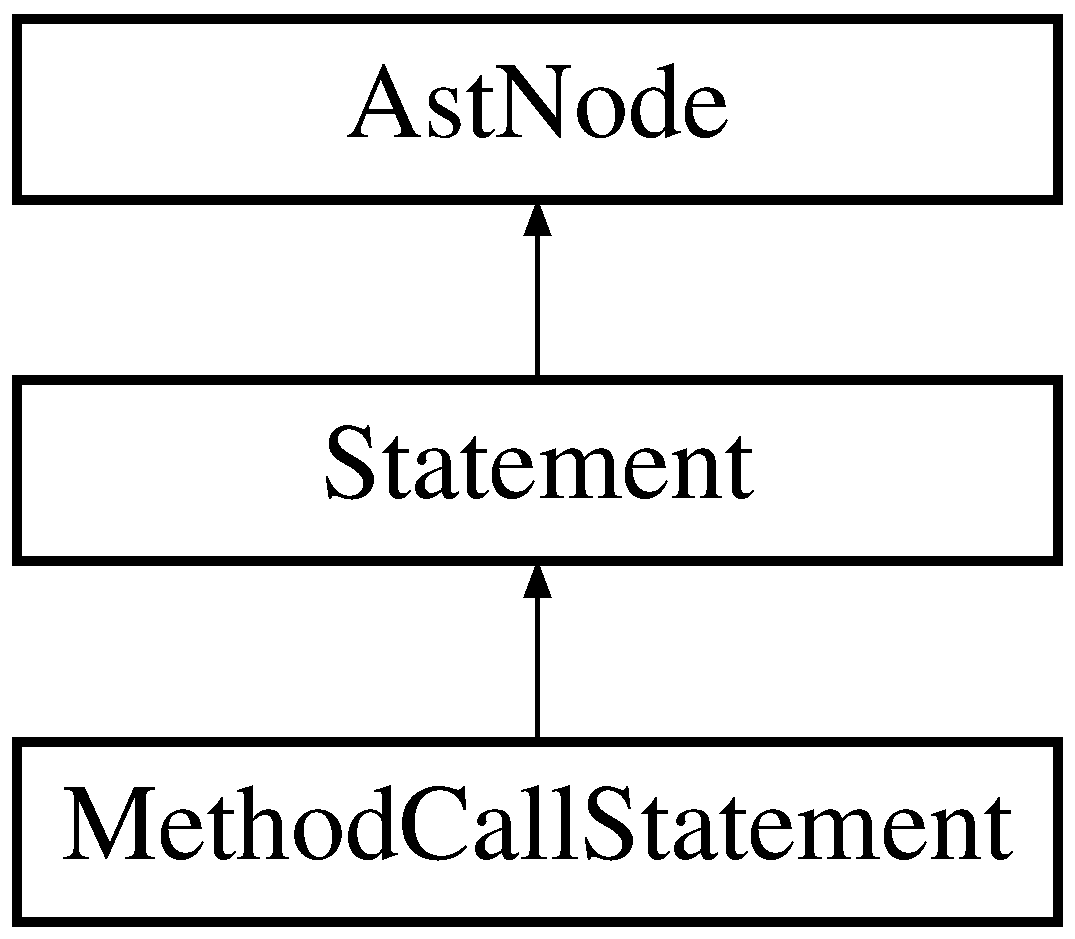
\includegraphics[height=3cm]{classMethodCallStatement}
\end{center}
\end{figure}
\subsection*{Public Member Functions}
\begin{DoxyCompactItemize}
\item 
\hyperlink{classMethodCallStatement_aa0ebf89fb7b2a464aed2685070578279}{MethodCallStatement} (int lno, \hyperlink{classExpression}{Expression} $\ast$e)
\item 
\hyperlink{classExpression}{Expression} $\ast$ \hyperlink{classMethodCallStatement_ab19af10f9dd979693f1714baf6f6e10f}{getExpression} ()
\item 
void \hyperlink{classMethodCallStatement_a4bbae8f172868a47ba651f436087e16f}{accept} (\hyperlink{classAstVisitor}{AstVisitor} $\ast$aVisitor)
\end{DoxyCompactItemize}


\subsection{Detailed Description}
This class represents a TinyJava method call statement. A method call statement node is a \char`\"{}wrapper\char`\"{} class used to represent a method call expression as a statement. 

\subsection{Constructor \& Destructor Documentation}
\hypertarget{classMethodCallStatement_aa0ebf89fb7b2a464aed2685070578279}{
\index{MethodCallStatement@{MethodCallStatement}!MethodCallStatement@{MethodCallStatement}}
\index{MethodCallStatement@{MethodCallStatement}!MethodCallStatement@{MethodCallStatement}}
\subsubsection[{MethodCallStatement}]{\setlength{\rightskip}{0pt plus 5cm}MethodCallStatement::MethodCallStatement (int {\em lno}, \/  {\bf Expression} $\ast$ {\em e})\hspace{0.3cm}{\ttfamily  \mbox{[}inline\mbox{]}}}}
\label{classMethodCallStatement_aa0ebf89fb7b2a464aed2685070578279}
Createa a new \hyperlink{classMethodCallStatement}{MethodCallStatement} object.


\begin{DoxyParams}{Parameters}
\item[{\em lno}]a source code line number with the method call statement. \item[{\em e}]a pointer to an \hyperlink{classExpression}{Expression} representing the \hyperlink{classMethodCallExpression}{MethodCallExpression} \end{DoxyParams}

\begin{DoxyExceptions}{Exceptions}
\item[{\em \hyperlink{classAstException}{AstException}}]if the e (\hyperlink{classExpression}{Expression}) argument is NULL or if it is not a \hyperlink{classMethodCallExpression}{MethodCallExpression} \end{DoxyExceptions}


\subsection{Member Function Documentation}
\hypertarget{classMethodCallStatement_a4bbae8f172868a47ba651f436087e16f}{
\index{MethodCallStatement@{MethodCallStatement}!accept@{accept}}
\index{accept@{accept}!MethodCallStatement@{MethodCallStatement}}
\subsubsection[{accept}]{\setlength{\rightskip}{0pt plus 5cm}void MethodCallStatement::accept ({\bf AstVisitor} $\ast$ {\em aVisitor})\hspace{0.3cm}{\ttfamily  \mbox{[}inline, virtual\mbox{]}}}}
\label{classMethodCallStatement_a4bbae8f172868a47ba651f436087e16f}
Accept a visitor to this node. 
\begin{DoxyParams}{Parameters}
\item[{\em aVisitor}]is a visitor object of type \hyperlink{classAstVisitor}{AstVisitor}. \end{DoxyParams}


Implements \hyperlink{classAstNode_a67b2d6ce1262da2954fb4db255759fb3}{AstNode}.\hypertarget{classMethodCallStatement_ab19af10f9dd979693f1714baf6f6e10f}{
\index{MethodCallStatement@{MethodCallStatement}!getExpression@{getExpression}}
\index{getExpression@{getExpression}!MethodCallStatement@{MethodCallStatement}}
\subsubsection[{getExpression}]{\setlength{\rightskip}{0pt plus 5cm}{\bf Expression}$\ast$ MethodCallStatement::getExpression ()\hspace{0.3cm}{\ttfamily  \mbox{[}inline\mbox{]}}}}
\label{classMethodCallStatement_ab19af10f9dd979693f1714baf6f6e10f}
Return the \hyperlink{classMethodCallExpression}{MethodCallExpression} of this \hyperlink{classMethodCallStatement}{MethodCallStatement}

\begin{DoxyReturn}{Returns}
a pointer to an \hyperlink{classExpression}{Expression} representing the \hyperlink{classMethodCallExpression}{MethodCallExpression} 
\end{DoxyReturn}


The documentation for this class was generated from the following file:\begin{DoxyCompactItemize}
\item 
MethodCallStmt.h\end{DoxyCompactItemize}

\hypertarget{classMethodDeclaration}{
\section{MethodDeclaration Class Reference}
\label{classMethodDeclaration}\index{MethodDeclaration@{MethodDeclaration}}
}


This class represents a method declaration in a TinyJava class.  


{\ttfamily \#include $<$MethodDeclaration.h$>$}Inheritance diagram for MethodDeclaration::\begin{figure}[H]
\begin{center}
\leavevmode
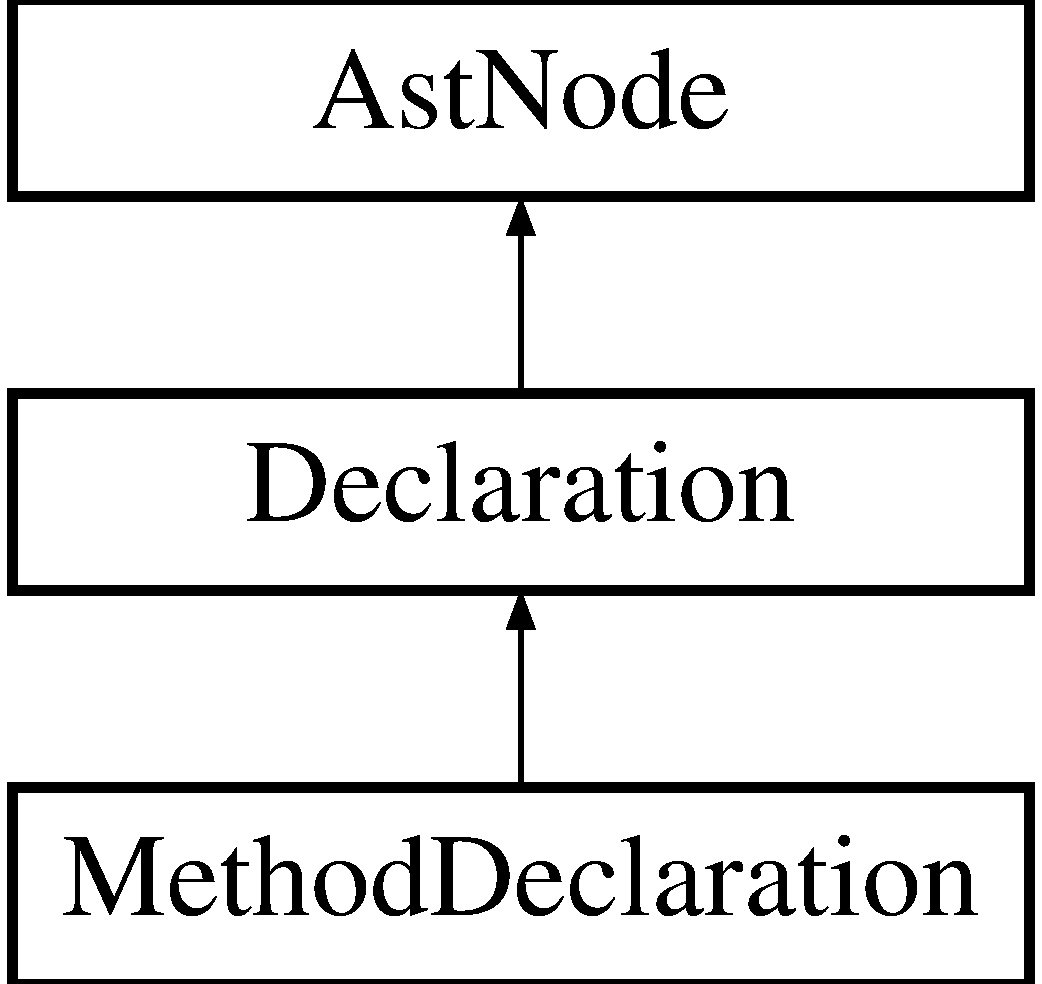
\includegraphics[height=3cm]{classMethodDeclaration}
\end{center}
\end{figure}
\subsection*{Public Member Functions}
\begin{DoxyCompactItemize}
\item 
\hyperlink{classMethodDeclaration_ae1ac6dc291290fc20f067360e275d3bb}{MethodDeclaration} (int lno, const char $\ast$nm, int rt)
\item 
const char $\ast$ \hyperlink{classMethodDeclaration_a792d1e64f2126f6daca537cb85e5ae6e}{getName} ()
\item 
bool \hyperlink{classMethodDeclaration_ac857d555077d6b35696470fd33f9315c}{isPublicMethod} ()
\item 
void \hyperlink{classMethodDeclaration_ad22630f0023935de4f76b0f399633ede}{setPublicMethod} (bool isPubliclyVisible)
\item 
int \hyperlink{classMethodDeclaration_ab26bfa7db28f171f2a25dacefd5141bf}{getRetType} ()
\item 
void \hyperlink{classMethodDeclaration_a82bce812810c881e6f1dca61b5b631ff}{setParameters} (std::vector$<$ \hyperlink{classDeclaration}{Declaration} $\ast$ $>$ $\ast$ps)
\item 
std::vector$<$ \hyperlink{classDeclaration}{Declaration} $\ast$ $>$ $\ast$ \hyperlink{classMethodDeclaration_ae57ec0b65b1edcaa7c6ddf5a08304886}{getParameters} ()
\item 
void \hyperlink{classMethodDeclaration_ad65f55276d3ea08cc0156a8a4eb3e035}{setVariables} (std::vector$<$ \hyperlink{classDeclaration}{Declaration} $\ast$ $>$ $\ast$vs)
\item 
std::vector$<$ \hyperlink{classDeclaration}{Declaration} $\ast$ $>$ $\ast$ \hyperlink{classMethodDeclaration_a4078ee50432bfa957007584cf6f3f260}{getVariables} ()
\item 
ENTRY $\ast$ \hyperlink{classMethodDeclaration_ab32ff62da9f19c145ad13f811b97b265}{getEntry} ()
\item 
void \hyperlink{classMethodDeclaration_aa786d4c52123cf501a85f2e3604f7cb6}{setEntry} (ENTRY $\ast$e)
\item 
\hyperlink{classStatement}{Statement} $\ast$ \hyperlink{classMethodDeclaration_a7c7b3d34df4197370caca80119f19c0f}{getBody} ()
\item 
void \hyperlink{classMethodDeclaration_a0ba428c0491f39c66a6b26d24077b56c}{setBody} (\hyperlink{classStatement}{Statement} $\ast$b)
\item 
void \hyperlink{classMethodDeclaration_af4989b6bfa1fdc87be33f4315aa54a7e}{accept} (\hyperlink{classAstVisitor}{AstVisitor} $\ast$aVisitor)
\end{DoxyCompactItemize}


\subsection{Detailed Description}
This class represents a method declaration in a TinyJava class. A method declaration is represented by:
\begin{DoxyItemize}
\item the method name (a string)
\item whether the method public or not
\item the return type of the method (an integer value, as defined in the \hyperlink{classAstNode}{AstNode} class)
\item formal parameters of the method (\hyperlink{classDeclaration}{Declaration} pointers)
\item local variables of the method (\hyperlink{classDeclaration}{Declaration} pointers)
\item body of the method (a pointer to a \hyperlink{classStatement}{Statement})
\end{DoxyItemize}

A pointer to the symbol table ENTRY for the method may also be included.

ENTRY should be defined as a macro, and its value should be a class, which is the root of the symbol table entry hierarchy. Its default value is Entry. The macro should be defined at the beginning of the header file Ast.h. 

\subsection{Constructor \& Destructor Documentation}
\hypertarget{classMethodDeclaration_ae1ac6dc291290fc20f067360e275d3bb}{
\index{MethodDeclaration@{MethodDeclaration}!MethodDeclaration@{MethodDeclaration}}
\index{MethodDeclaration@{MethodDeclaration}!MethodDeclaration@{MethodDeclaration}}
\subsubsection[{MethodDeclaration}]{\setlength{\rightskip}{0pt plus 5cm}MethodDeclaration::MethodDeclaration (int {\em lno}, \/  const char $\ast$ {\em nm}, \/  int {\em rt})}}
\label{classMethodDeclaration_ae1ac6dc291290fc20f067360e275d3bb}
Create a new \hyperlink{classMethodDeclaration}{MethodDeclaration} object. The method body is set to NULL. The symbol table ENTRY pointer is set to NULL. No parameters or local variables are created.


\begin{DoxyParams}{Parameters}
\item[{\em lno}]a source code line number with the method declaration (should be the beginning of the method) \item[{\em nm}]a string representing the method name \item[{\em rt}]a integer value representing the return type, as defined in the \hyperlink{classAstNode}{AstNode} class \end{DoxyParams}

\begin{DoxyExceptions}{Exceptions}
\item[{\em \hyperlink{classAstException}{AstException}}]if the method name is NULL \end{DoxyExceptions}


\subsection{Member Function Documentation}
\hypertarget{classMethodDeclaration_af4989b6bfa1fdc87be33f4315aa54a7e}{
\index{MethodDeclaration@{MethodDeclaration}!accept@{accept}}
\index{accept@{accept}!MethodDeclaration@{MethodDeclaration}}
\subsubsection[{accept}]{\setlength{\rightskip}{0pt plus 5cm}void MethodDeclaration::accept ({\bf AstVisitor} $\ast$ {\em aVisitor})\hspace{0.3cm}{\ttfamily  \mbox{[}inline, virtual\mbox{]}}}}
\label{classMethodDeclaration_af4989b6bfa1fdc87be33f4315aa54a7e}
Accept a visitor to this node. 
\begin{DoxyParams}{Parameters}
\item[{\em aVisitor}]is a visitor object of type \hyperlink{classAstVisitor}{AstVisitor}. \end{DoxyParams}


Implements \hyperlink{classAstNode_a67b2d6ce1262da2954fb4db255759fb3}{AstNode}.\hypertarget{classMethodDeclaration_a7c7b3d34df4197370caca80119f19c0f}{
\index{MethodDeclaration@{MethodDeclaration}!getBody@{getBody}}
\index{getBody@{getBody}!MethodDeclaration@{MethodDeclaration}}
\subsubsection[{getBody}]{\setlength{\rightskip}{0pt plus 5cm}{\bf Statement}$\ast$ MethodDeclaration::getBody ()\hspace{0.3cm}{\ttfamily  \mbox{[}inline\mbox{]}}}}
\label{classMethodDeclaration_a7c7b3d34df4197370caca80119f19c0f}
Return the body of this method

\begin{DoxyReturn}{Returns}
pointer to a \hyperlink{classStatement}{Statement} representing the body of the method 
\end{DoxyReturn}
\hypertarget{classMethodDeclaration_ab32ff62da9f19c145ad13f811b97b265}{
\index{MethodDeclaration@{MethodDeclaration}!getEntry@{getEntry}}
\index{getEntry@{getEntry}!MethodDeclaration@{MethodDeclaration}}
\subsubsection[{getEntry}]{\setlength{\rightskip}{0pt plus 5cm}ENTRY$\ast$ MethodDeclaration::getEntry ()\hspace{0.3cm}{\ttfamily  \mbox{[}inline\mbox{]}}}}
\label{classMethodDeclaration_ab32ff62da9f19c145ad13f811b97b265}
Return a pointer to the symbol table ENTRY representing this method declaration. This value may be undefined before the symbol table is created.

\begin{DoxyReturn}{Returns}
a pointer to the symbol table entry representing this method declaration. 
\end{DoxyReturn}
\hypertarget{classMethodDeclaration_a792d1e64f2126f6daca537cb85e5ae6e}{
\index{MethodDeclaration@{MethodDeclaration}!getName@{getName}}
\index{getName@{getName}!MethodDeclaration@{MethodDeclaration}}
\subsubsection[{getName}]{\setlength{\rightskip}{0pt plus 5cm}const char$\ast$ MethodDeclaration::getName ()\hspace{0.3cm}{\ttfamily  \mbox{[}inline\mbox{]}}}}
\label{classMethodDeclaration_a792d1e64f2126f6daca537cb85e5ae6e}
Return the method name.

\begin{DoxyReturn}{Returns}
string representing the method name. 
\end{DoxyReturn}
\hypertarget{classMethodDeclaration_ae57ec0b65b1edcaa7c6ddf5a08304886}{
\index{MethodDeclaration@{MethodDeclaration}!getParameters@{getParameters}}
\index{getParameters@{getParameters}!MethodDeclaration@{MethodDeclaration}}
\subsubsection[{getParameters}]{\setlength{\rightskip}{0pt plus 5cm}std::vector$<${\bf Declaration} $\ast$$>$$\ast$ MethodDeclaration::getParameters ()\hspace{0.3cm}{\ttfamily  \mbox{[}inline\mbox{]}}}}
\label{classMethodDeclaration_ae57ec0b65b1edcaa7c6ddf5a08304886}
Return all formal parameters of this method.

\begin{DoxyReturn}{Returns}
a pointer to a std::vector with pointers referencing ParameterDeclarations of this method 
\end{DoxyReturn}
\hypertarget{classMethodDeclaration_ab26bfa7db28f171f2a25dacefd5141bf}{
\index{MethodDeclaration@{MethodDeclaration}!getRetType@{getRetType}}
\index{getRetType@{getRetType}!MethodDeclaration@{MethodDeclaration}}
\subsubsection[{getRetType}]{\setlength{\rightskip}{0pt plus 5cm}int MethodDeclaration::getRetType ()\hspace{0.3cm}{\ttfamily  \mbox{[}inline\mbox{]}}}}
\label{classMethodDeclaration_ab26bfa7db28f171f2a25dacefd5141bf}
Return the type of this method declaration node.

\begin{DoxyReturn}{Returns}
an integer value representing the method return type, as defined in the \hyperlink{classAstNode}{AstNode} class. 
\end{DoxyReturn}
\hypertarget{classMethodDeclaration_a4078ee50432bfa957007584cf6f3f260}{
\index{MethodDeclaration@{MethodDeclaration}!getVariables@{getVariables}}
\index{getVariables@{getVariables}!MethodDeclaration@{MethodDeclaration}}
\subsubsection[{getVariables}]{\setlength{\rightskip}{0pt plus 5cm}std::vector$<${\bf Declaration} $\ast$$>$$\ast$ MethodDeclaration::getVariables ()\hspace{0.3cm}{\ttfamily  \mbox{[}inline\mbox{]}}}}
\label{classMethodDeclaration_a4078ee50432bfa957007584cf6f3f260}
Return all local variables of this method.

\begin{DoxyReturn}{Returns}
a pointer to a std::vector with pointers referencing VariableDeclarations of this method 
\end{DoxyReturn}
\hypertarget{classMethodDeclaration_ac857d555077d6b35696470fd33f9315c}{
\index{MethodDeclaration@{MethodDeclaration}!isPublicMethod@{isPublicMethod}}
\index{isPublicMethod@{isPublicMethod}!MethodDeclaration@{MethodDeclaration}}
\subsubsection[{isPublicMethod}]{\setlength{\rightskip}{0pt plus 5cm}bool MethodDeclaration::isPublicMethod ()\hspace{0.3cm}{\ttfamily  \mbox{[}inline\mbox{]}}}}
\label{classMethodDeclaration_ac857d555077d6b35696470fd33f9315c}
Is the method public?

\begin{DoxyReturn}{Returns}
a boolean value representing the method's public visibility status 
\end{DoxyReturn}
\hypertarget{classMethodDeclaration_a0ba428c0491f39c66a6b26d24077b56c}{
\index{MethodDeclaration@{MethodDeclaration}!setBody@{setBody}}
\index{setBody@{setBody}!MethodDeclaration@{MethodDeclaration}}
\subsubsection[{setBody}]{\setlength{\rightskip}{0pt plus 5cm}void MethodDeclaration::setBody ({\bf Statement} $\ast$ {\em b})\hspace{0.3cm}{\ttfamily  \mbox{[}inline\mbox{]}}}}
\label{classMethodDeclaration_a0ba428c0491f39c66a6b26d24077b56c}
Set the body of thie method


\begin{DoxyParams}{Parameters}
\item[{\em b}]a \hyperlink{classStatement}{Statement} pointer representing the body of the method; must be a pointer to \hyperlink{classBlockStatement}{BlockStatement} \end{DoxyParams}

\begin{DoxyExceptions}{Exceptions}
\item[{\em \hyperlink{classAstException}{AstException}}]if the argument b is NULL or if it is not a \hyperlink{classBlockStatement}{BlockStatement} \end{DoxyExceptions}
\hypertarget{classMethodDeclaration_aa786d4c52123cf501a85f2e3604f7cb6}{
\index{MethodDeclaration@{MethodDeclaration}!setEntry@{setEntry}}
\index{setEntry@{setEntry}!MethodDeclaration@{MethodDeclaration}}
\subsubsection[{setEntry}]{\setlength{\rightskip}{0pt plus 5cm}void MethodDeclaration::setEntry (ENTRY $\ast$ {\em e})\hspace{0.3cm}{\ttfamily  \mbox{[}inline\mbox{]}}}}
\label{classMethodDeclaration_aa786d4c52123cf501a85f2e3604f7cb6}
Set the pointer to the symbol table entry representing this method declaration. This value will typically be set during the symbol table construction phase.


\begin{DoxyParams}{Parameters}
\item[{\em e}]the pointer to the symbol table entry representing this method declaration. \end{DoxyParams}
\hypertarget{classMethodDeclaration_a82bce812810c881e6f1dca61b5b631ff}{
\index{MethodDeclaration@{MethodDeclaration}!setParameters@{setParameters}}
\index{setParameters@{setParameters}!MethodDeclaration@{MethodDeclaration}}
\subsubsection[{setParameters}]{\setlength{\rightskip}{0pt plus 5cm}void MethodDeclaration::setParameters (std::vector$<$ {\bf Declaration} $\ast$ $>$ $\ast$ {\em ps})}}
\label{classMethodDeclaration_a82bce812810c881e6f1dca61b5b631ff}
Set the formal parameters of this method declaration


\begin{DoxyParams}{Parameters}
\item[{\em ps}]a pointer to a std::vector of \hyperlink{classParameterDeclaration}{ParameterDeclaration} pointers, each representing a formal parameter declaration \end{DoxyParams}

\begin{DoxyExceptions}{Exceptions}
\item[{\em \hyperlink{classAstException}{AstException}}]if any of the \hyperlink{classDeclaration}{Declaration} pointers in the argument std::vector is NULL or is not a \hyperlink{classParameterDeclaration}{ParameterDeclaration} \end{DoxyExceptions}
\hypertarget{classMethodDeclaration_ad22630f0023935de4f76b0f399633ede}{
\index{MethodDeclaration@{MethodDeclaration}!setPublicMethod@{setPublicMethod}}
\index{setPublicMethod@{setPublicMethod}!MethodDeclaration@{MethodDeclaration}}
\subsubsection[{setPublicMethod}]{\setlength{\rightskip}{0pt plus 5cm}void MethodDeclaration::setPublicMethod (bool {\em isPubliclyVisible})\hspace{0.3cm}{\ttfamily  \mbox{[}inline\mbox{]}}}}
\label{classMethodDeclaration_ad22630f0023935de4f76b0f399633ede}
Set the public visibility status of this method


\begin{DoxyParams}{Parameters}
\item[{\em isPubliclyVisible}]the new public visibility status \end{DoxyParams}
\hypertarget{classMethodDeclaration_ad65f55276d3ea08cc0156a8a4eb3e035}{
\index{MethodDeclaration@{MethodDeclaration}!setVariables@{setVariables}}
\index{setVariables@{setVariables}!MethodDeclaration@{MethodDeclaration}}
\subsubsection[{setVariables}]{\setlength{\rightskip}{0pt plus 5cm}void MethodDeclaration::setVariables (std::vector$<$ {\bf Declaration} $\ast$ $>$ $\ast$ {\em vs})}}
\label{classMethodDeclaration_ad65f55276d3ea08cc0156a8a4eb3e035}
Set the local variables of this method declaration


\begin{DoxyParams}{Parameters}
\item[{\em vs}]a pointer to a std::vector of \hyperlink{classVariableDeclaration}{VariableDeclaration} pointers, each representing a local variable declaration \end{DoxyParams}

\begin{DoxyExceptions}{Exceptions}
\item[{\em \hyperlink{classAstException}{AstException}}]if any of the \hyperlink{classDeclaration}{Declaration} pointers in the argument std::vector is NULL or is not a \hyperlink{classVariableDeclaration}{VariableDeclaration} \end{DoxyExceptions}


The documentation for this class was generated from the following files:\begin{DoxyCompactItemize}
\item 
MethodDeclaration.h\item 
MethodDeclaration.cpp\end{DoxyCompactItemize}

\hypertarget{classNewExpression}{
\section{NewExpression Class Reference}
\label{classNewExpression}\index{NewExpression@{NewExpression}}
}


This class represents a TinyJava NEW expression (used for array creation).  


{\ttfamily \#include $<$NewExpression.h$>$}Inheritance diagram for NewExpression::\begin{figure}[H]
\begin{center}
\leavevmode
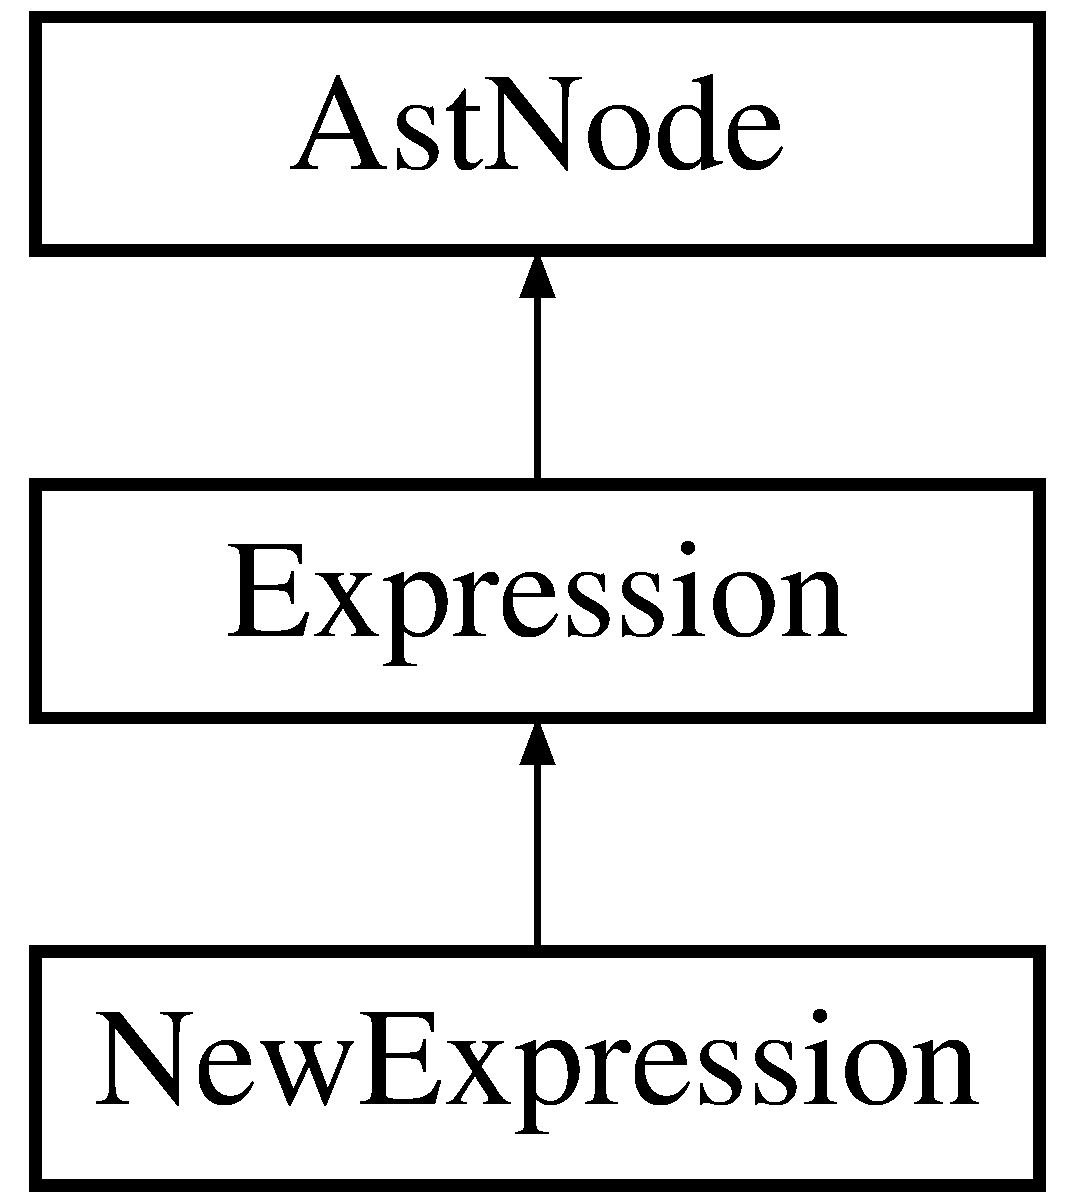
\includegraphics[height=3cm]{classNewExpression}
\end{center}
\end{figure}
\subsection*{Public Member Functions}
\begin{DoxyCompactItemize}
\item 
\hyperlink{classNewExpression_a19c967d630d86b4ff25b95e589d3a84d}{NewExpression} (int lno, int tp, \hyperlink{classExpression}{Expression} $\ast$size)
\item 
int \hyperlink{classNewExpression_aa26ede4c3685e4cf1846eb62b9051355}{getBaseType} ()
\item 
\hyperlink{classExpression}{Expression} $\ast$ \hyperlink{classNewExpression_a86da8a128d8c401ba775cd997aa634fa}{getExpression} ()
\item 
void \hyperlink{classNewExpression_a187b0a20b76ebd542c84b43880ef9692}{setExpression} (\hyperlink{classExpression}{Expression} $\ast$arg)
\item 
void \hyperlink{classNewExpression_a4b5178e78150432ac58a08197204fa27}{accept} (\hyperlink{classAstVisitor}{AstVisitor} $\ast$aVisitor)
\end{DoxyCompactItemize}


\subsection{Detailed Description}
This class represents a TinyJava NEW expression (used for array creation). A \hyperlink{classNewExpression}{NewExpression} is represented by:
\begin{DoxyItemize}
\item the constructed type (i.e. array base type)
\item an \hyperlink{classExpression}{Expression} representing the size of the array to be created 
\end{DoxyItemize}

\subsection{Constructor \& Destructor Documentation}
\hypertarget{classNewExpression_a19c967d630d86b4ff25b95e589d3a84d}{
\index{NewExpression@{NewExpression}!NewExpression@{NewExpression}}
\index{NewExpression@{NewExpression}!NewExpression@{NewExpression}}
\subsubsection[{NewExpression}]{\setlength{\rightskip}{0pt plus 5cm}NewExpression::NewExpression (int {\em lno}, \/  int {\em tp}, \/  {\bf Expression} $\ast$ {\em size})\hspace{0.3cm}{\ttfamily  \mbox{[}inline\mbox{]}}}}
\label{classNewExpression_a19c967d630d86b4ff25b95e589d3a84d}
Create a new \hyperlink{classNewExpression}{NewExpression} object


\begin{DoxyParams}{Parameters}
\item[{\em lno}]a source line number containing the new expression \item[{\em tp}]the type of the created value (array base type), as defined in the \hyperlink{classAstNode}{AstNode} class \item[{\em size}]a pointer to \hyperlink{classExpression}{Expression} representing the size of the new array \end{DoxyParams}

\begin{DoxyExceptions}{Exceptions}
\item[{\em \hyperlink{classAstException}{AstException}}]if the size \hyperlink{classExpression}{Expression} is NULL \end{DoxyExceptions}


\subsection{Member Function Documentation}
\hypertarget{classNewExpression_a4b5178e78150432ac58a08197204fa27}{
\index{NewExpression@{NewExpression}!accept@{accept}}
\index{accept@{accept}!NewExpression@{NewExpression}}
\subsubsection[{accept}]{\setlength{\rightskip}{0pt plus 5cm}void NewExpression::accept ({\bf AstVisitor} $\ast$ {\em aVisitor})\hspace{0.3cm}{\ttfamily  \mbox{[}inline, virtual\mbox{]}}}}
\label{classNewExpression_a4b5178e78150432ac58a08197204fa27}
Accept a visitor to this node. 
\begin{DoxyParams}{Parameters}
\item[{\em aVisitor}]is a visitor object of type \hyperlink{classAstVisitor}{AstVisitor}. \end{DoxyParams}


Implements \hyperlink{classAstNode_a67b2d6ce1262da2954fb4db255759fb3}{AstNode}.\hypertarget{classNewExpression_aa26ede4c3685e4cf1846eb62b9051355}{
\index{NewExpression@{NewExpression}!getBaseType@{getBaseType}}
\index{getBaseType@{getBaseType}!NewExpression@{NewExpression}}
\subsubsection[{getBaseType}]{\setlength{\rightskip}{0pt plus 5cm}int NewExpression::getBaseType ()\hspace{0.3cm}{\ttfamily  \mbox{[}inline\mbox{]}}}}
\label{classNewExpression_aa26ede4c3685e4cf1846eb62b9051355}
Return the type to be created (array base type)

\begin{DoxyReturn}{Returns}
an integer value representing the type, as defined in the \hyperlink{classAstNode}{AstNode} class. 
\end{DoxyReturn}
\hypertarget{classNewExpression_a86da8a128d8c401ba775cd997aa634fa}{
\index{NewExpression@{NewExpression}!getExpression@{getExpression}}
\index{getExpression@{getExpression}!NewExpression@{NewExpression}}
\subsubsection[{getExpression}]{\setlength{\rightskip}{0pt plus 5cm}{\bf Expression}$\ast$ NewExpression::getExpression ()\hspace{0.3cm}{\ttfamily  \mbox{[}inline\mbox{]}}}}
\label{classNewExpression_a86da8a128d8c401ba775cd997aa634fa}
Return the size \hyperlink{classExpression}{Expression}

\begin{DoxyReturn}{Returns}
a pointer to \hyperlink{classExpression}{Expression} representing the array size 
\end{DoxyReturn}
\hypertarget{classNewExpression_a187b0a20b76ebd542c84b43880ef9692}{
\index{NewExpression@{NewExpression}!setExpression@{setExpression}}
\index{setExpression@{setExpression}!NewExpression@{NewExpression}}
\subsubsection[{setExpression}]{\setlength{\rightskip}{0pt plus 5cm}void NewExpression::setExpression ({\bf Expression} $\ast$ {\em arg})\hspace{0.3cm}{\ttfamily  \mbox{[}inline\mbox{]}}}}
\label{classNewExpression_a187b0a20b76ebd542c84b43880ef9692}
Set the size \hyperlink{classExpression}{Expression}


\begin{DoxyParams}{Parameters}
\item[{\em arg}]is a pointer to an \hyperlink{classExpression}{Expression} representing the array size \end{DoxyParams}

\begin{DoxyExceptions}{Exceptions}
\item[{\em \hyperlink{classAstException}{AstException}}]if the arg \hyperlink{classExpression}{Expression} is NULL \end{DoxyExceptions}


The documentation for this class was generated from the following file:\begin{DoxyCompactItemize}
\item 
NewExpression.h\end{DoxyCompactItemize}

\hypertarget{classParameterDeclaration}{
\section{ParameterDeclaration Class Reference}
\label{classParameterDeclaration}\index{ParameterDeclaration@{ParameterDeclaration}}
}


This class represents a declaration of a formal parameter of a TinyJava class method.  


{\ttfamily \#include $<$ParameterDeclaration.h$>$}Inheritance diagram for ParameterDeclaration::\begin{figure}[H]
\begin{center}
\leavevmode
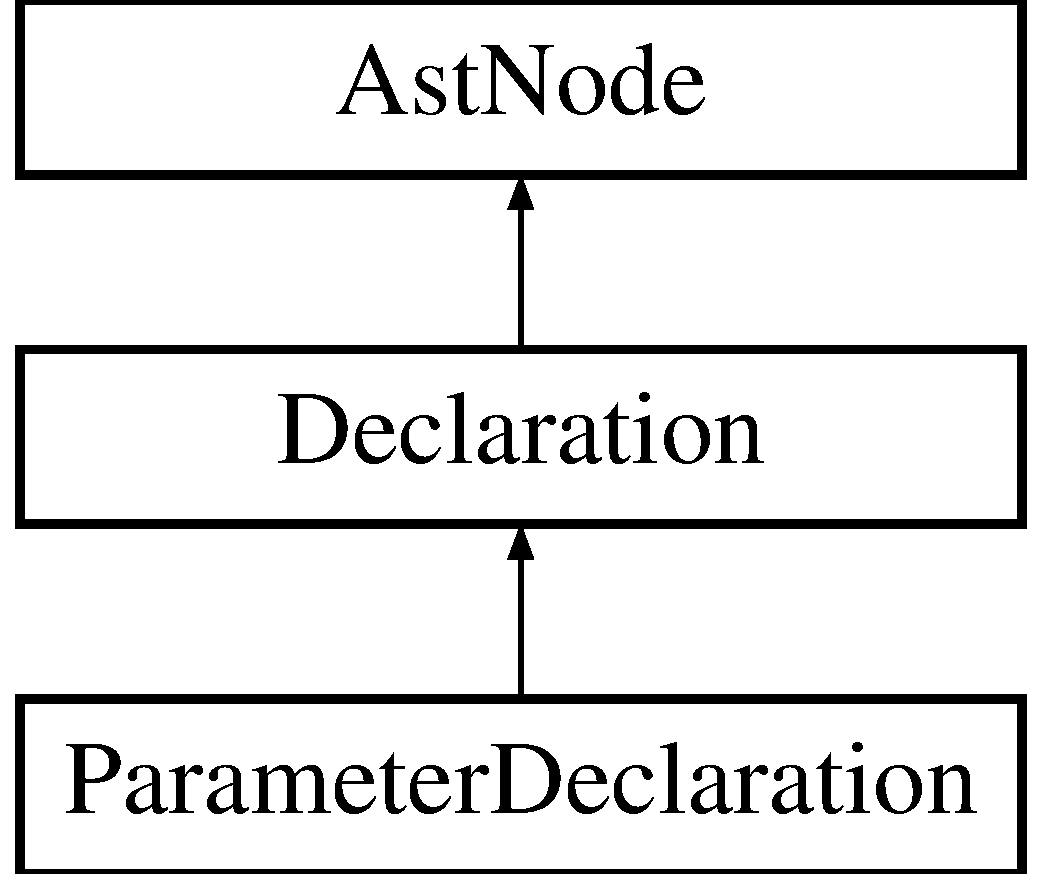
\includegraphics[height=3cm]{classParameterDeclaration}
\end{center}
\end{figure}
\subsection*{Public Member Functions}
\begin{DoxyCompactItemize}
\item 
\hyperlink{classParameterDeclaration_ac1212fec82bbbcb3d965f6b21ba0f814}{ParameterDeclaration} (int lno, const char $\ast$nm, int tp)
\item 
const char $\ast$ \hyperlink{classParameterDeclaration_ae8b4050a45ff9671d5bc4020ce8a921f}{getName} ()
\item 
void \hyperlink{classParameterDeclaration_a1883647c68399feaffb9531e27b85bb2}{setName} (const char $\ast$nm)
\item 
int \hyperlink{classParameterDeclaration_a68cbaf66b6aa35c05fc30f236321829a}{getType} ()
\item 
void \hyperlink{classParameterDeclaration_aee125114f14e0bcfaa15753d6b1379cf}{setType} (int tp)
\item 
ENTRY $\ast$ \hyperlink{classParameterDeclaration_a80ec2ae28260deaa1925f3de51c620a8}{getEntry} ()
\item 
void \hyperlink{classParameterDeclaration_a8b07142bec67be6eccd2bdf3147fb5a2}{setEntry} (ENTRY $\ast$e)
\item 
void \hyperlink{classParameterDeclaration_a7e9679286d169930445a159abd5e42ad}{accept} (\hyperlink{classAstVisitor}{AstVisitor} $\ast$aVisitor)
\end{DoxyCompactItemize}


\subsection{Detailed Description}
This class represents a declaration of a formal parameter of a TinyJava class method. A parameter is represented by:
\begin{DoxyItemize}
\item parameter name -\/ a string
\item type -\/ an integer value, as defined in the \hyperlink{classAstNode}{AstNode} class
\item a pointer to the symbol table ENTRY for the variable (which may be initially undefined).
\end{DoxyItemize}

ENTRY should be defined as a macro, and its value should be a class, which is the root of the symbol table entry hierarchy. Its default value is Entry. The macro should be defined at the beginning of the header file Ast.h. 

\subsection{Constructor \& Destructor Documentation}
\hypertarget{classParameterDeclaration_ac1212fec82bbbcb3d965f6b21ba0f814}{
\index{ParameterDeclaration@{ParameterDeclaration}!ParameterDeclaration@{ParameterDeclaration}}
\index{ParameterDeclaration@{ParameterDeclaration}!ParameterDeclaration@{ParameterDeclaration}}
\subsubsection[{ParameterDeclaration}]{\setlength{\rightskip}{0pt plus 5cm}ParameterDeclaration::ParameterDeclaration (int {\em lno}, \/  const char $\ast$ {\em nm}, \/  int {\em tp})\hspace{0.3cm}{\ttfamily  \mbox{[}inline\mbox{]}}}}
\label{classParameterDeclaration_ac1212fec82bbbcb3d965f6b21ba0f814}
Create a new \hyperlink{classParameterDeclaration}{ParameterDeclaration} object.


\begin{DoxyParams}{Parameters}
\item[{\em lno}]a source code line number with the parameter declaration. \item[{\em nm}]a string with the parameter name \item[{\em tp}]an integer representing the type, as defined in the \hyperlink{classAstNode}{AstNode} class \end{DoxyParams}

\begin{DoxyExceptions}{Exceptions}
\item[{\em \hyperlink{classAstException}{AstException}}]if the parameter name is NULL \end{DoxyExceptions}


\subsection{Member Function Documentation}
\hypertarget{classParameterDeclaration_a7e9679286d169930445a159abd5e42ad}{
\index{ParameterDeclaration@{ParameterDeclaration}!accept@{accept}}
\index{accept@{accept}!ParameterDeclaration@{ParameterDeclaration}}
\subsubsection[{accept}]{\setlength{\rightskip}{0pt plus 5cm}void ParameterDeclaration::accept ({\bf AstVisitor} $\ast$ {\em aVisitor})\hspace{0.3cm}{\ttfamily  \mbox{[}inline, virtual\mbox{]}}}}
\label{classParameterDeclaration_a7e9679286d169930445a159abd5e42ad}
Accept a visitor to this node. 
\begin{DoxyParams}{Parameters}
\item[{\em aVisitor}]is a visitor object of type \hyperlink{classAstVisitor}{AstVisitor}. \end{DoxyParams}


Implements \hyperlink{classAstNode_a67b2d6ce1262da2954fb4db255759fb3}{AstNode}.\hypertarget{classParameterDeclaration_a80ec2ae28260deaa1925f3de51c620a8}{
\index{ParameterDeclaration@{ParameterDeclaration}!getEntry@{getEntry}}
\index{getEntry@{getEntry}!ParameterDeclaration@{ParameterDeclaration}}
\subsubsection[{getEntry}]{\setlength{\rightskip}{0pt plus 5cm}ENTRY$\ast$ ParameterDeclaration::getEntry ()\hspace{0.3cm}{\ttfamily  \mbox{[}inline\mbox{]}}}}
\label{classParameterDeclaration_a80ec2ae28260deaa1925f3de51c620a8}
Return a pointer to the symbol table ENTRY representing this parameter This value may be undefined before the symbol table is created.

\begin{DoxyReturn}{Returns}
a pointer to the symbol table ENTRY representing this parameter 
\end{DoxyReturn}
\hypertarget{classParameterDeclaration_ae8b4050a45ff9671d5bc4020ce8a921f}{
\index{ParameterDeclaration@{ParameterDeclaration}!getName@{getName}}
\index{getName@{getName}!ParameterDeclaration@{ParameterDeclaration}}
\subsubsection[{getName}]{\setlength{\rightskip}{0pt plus 5cm}const char$\ast$ ParameterDeclaration::getName ()\hspace{0.3cm}{\ttfamily  \mbox{[}inline\mbox{]}}}}
\label{classParameterDeclaration_ae8b4050a45ff9671d5bc4020ce8a921f}
Return the parameter name.

\begin{DoxyReturn}{Returns}
string representing the parameter name. 
\end{DoxyReturn}
\hypertarget{classParameterDeclaration_a68cbaf66b6aa35c05fc30f236321829a}{
\index{ParameterDeclaration@{ParameterDeclaration}!getType@{getType}}
\index{getType@{getType}!ParameterDeclaration@{ParameterDeclaration}}
\subsubsection[{getType}]{\setlength{\rightskip}{0pt plus 5cm}int ParameterDeclaration::getType ()\hspace{0.3cm}{\ttfamily  \mbox{[}inline\mbox{]}}}}
\label{classParameterDeclaration_a68cbaf66b6aa35c05fc30f236321829a}
Return the type of this \hyperlink{classParameterDeclaration}{ParameterDeclaration}.

\begin{DoxyReturn}{Returns}
an integer value representing the type, as defined in the \hyperlink{classAstNode}{AstNode} class. 
\end{DoxyReturn}
\hypertarget{classParameterDeclaration_a8b07142bec67be6eccd2bdf3147fb5a2}{
\index{ParameterDeclaration@{ParameterDeclaration}!setEntry@{setEntry}}
\index{setEntry@{setEntry}!ParameterDeclaration@{ParameterDeclaration}}
\subsubsection[{setEntry}]{\setlength{\rightskip}{0pt plus 5cm}void ParameterDeclaration::setEntry (ENTRY $\ast$ {\em e})\hspace{0.3cm}{\ttfamily  \mbox{[}inline\mbox{]}}}}
\label{classParameterDeclaration_a8b07142bec67be6eccd2bdf3147fb5a2}
Set the pointer to the symbol table ENTRY representing this parameter. This value will typically be set during the symbol table construction phase.


\begin{DoxyParams}{Parameters}
\item[{\em e}]the pointer to the symbol table ENTRY representing this parameter \end{DoxyParams}
\hypertarget{classParameterDeclaration_a1883647c68399feaffb9531e27b85bb2}{
\index{ParameterDeclaration@{ParameterDeclaration}!setName@{setName}}
\index{setName@{setName}!ParameterDeclaration@{ParameterDeclaration}}
\subsubsection[{setName}]{\setlength{\rightskip}{0pt plus 5cm}void ParameterDeclaration::setName (const char $\ast$ {\em nm})\hspace{0.3cm}{\ttfamily  \mbox{[}inline\mbox{]}}}}
\label{classParameterDeclaration_a1883647c68399feaffb9531e27b85bb2}
Set the parameter name.


\begin{DoxyParams}{Parameters}
\item[{\em nm}]a string representing the new name of the parameter \end{DoxyParams}
\hypertarget{classParameterDeclaration_aee125114f14e0bcfaa15753d6b1379cf}{
\index{ParameterDeclaration@{ParameterDeclaration}!setType@{setType}}
\index{setType@{setType}!ParameterDeclaration@{ParameterDeclaration}}
\subsubsection[{setType}]{\setlength{\rightskip}{0pt plus 5cm}void ParameterDeclaration::setType (int {\em tp})\hspace{0.3cm}{\ttfamily  \mbox{[}inline\mbox{]}}}}
\label{classParameterDeclaration_aee125114f14e0bcfaa15753d6b1379cf}
Set the new type of this \hyperlink{classParameterDeclaration}{ParameterDeclaration}.


\begin{DoxyParams}{Parameters}
\item[{\em tp}]an integer value representing the type, as defined in the \hyperlink{classAstNode}{AstNode} class. \end{DoxyParams}


The documentation for this class was generated from the following file:\begin{DoxyCompactItemize}
\item 
ParameterDeclaration.h\end{DoxyCompactItemize}

\hypertarget{classReferenceExpression}{
\section{ReferenceExpression Class Reference}
\label{classReferenceExpression}\index{ReferenceExpression@{ReferenceExpression}}
}


This class represents an identifier reference in a TinyJava expression; may be an array element reference with an index (subscript) expression.  


{\ttfamily \#include $<$ReferenceExpression.h$>$}Inheritance diagram for ReferenceExpression::\begin{figure}[H]
\begin{center}
\leavevmode
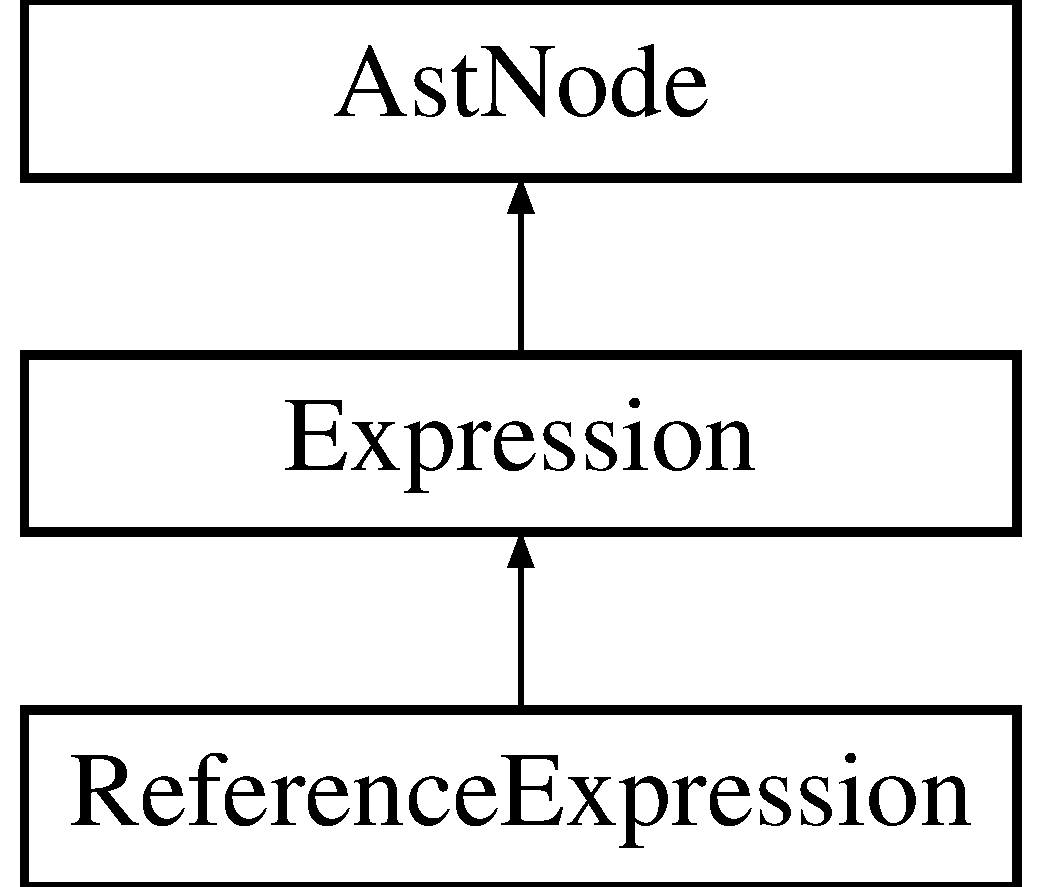
\includegraphics[height=3cm]{classReferenceExpression}
\end{center}
\end{figure}
\subsection*{Public Member Functions}
\begin{DoxyCompactItemize}
\item 
\hyperlink{classReferenceExpression_a7f614ef621f7336070a5a0f495475cce}{ReferenceExpression} (int lno, const char $\ast$n)
\item 
\hyperlink{classReferenceExpression_a374d0940a132e2c36b96f502354822af}{ReferenceExpression} (int lno, const char $\ast$n, \hyperlink{classExpression}{Expression} $\ast$ex)
\item 
const char $\ast$ \hyperlink{classReferenceExpression_a5a5123067be08b29efb72db0a3c59ec0}{getName} ()
\item 
ENTRY $\ast$ \hyperlink{classReferenceExpression_aaa972751c0253013518547cf6efaa513}{getEntry} ()
\item 
void \hyperlink{classReferenceExpression_a764220182810e4b7d0ec4b5f294d08f8}{setEntry} (ENTRY $\ast$e)
\item 
\hyperlink{classExpression}{Expression} $\ast$ \hyperlink{classReferenceExpression_a88b28a401551edd1cd4462df16ce8a51}{getExpression} ()
\item 
void \hyperlink{classReferenceExpression_a5235ddeb368f790fd69b73dc1fe5a80e}{accept} (\hyperlink{classAstVisitor}{AstVisitor} $\ast$aVisitor)
\end{DoxyCompactItemize}


\subsection{Detailed Description}
This class represents an identifier reference in a TinyJava expression; may be an array element reference with an index (subscript) expression. A referred identifier may be either a class field, a method parameter, or a local variable. It may also be a reference to an array alement. A \hyperlink{classReferenceExpression}{ReferenceExpression} is usually a leaf in an Abstract Syntax Tree.

A reference expression representation has:
\begin{DoxyItemize}
\item a string representing the referenced name (a variable, parameter, or a class field);
\item an index (subscript) expression, if the reference is to an array element
\item a pointer to the symbol table entry for the name may also be included. 
\end{DoxyItemize}

\subsection{Constructor \& Destructor Documentation}
\hypertarget{classReferenceExpression_a7f614ef621f7336070a5a0f495475cce}{
\index{ReferenceExpression@{ReferenceExpression}!ReferenceExpression@{ReferenceExpression}}
\index{ReferenceExpression@{ReferenceExpression}!ReferenceExpression@{ReferenceExpression}}
\subsubsection[{ReferenceExpression}]{\setlength{\rightskip}{0pt plus 5cm}ReferenceExpression::ReferenceExpression (int {\em lno}, \/  const char $\ast$ {\em n})\hspace{0.3cm}{\ttfamily  \mbox{[}inline\mbox{]}}}}
\label{classReferenceExpression_a7f614ef621f7336070a5a0f495475cce}
Create a new \hyperlink{classReferenceExpression}{ReferenceExpression} object.


\begin{DoxyParams}{Parameters}
\item[{\em lno}]is a source line number with the referenced identifier \item[{\em n}]is a string representing the name \end{DoxyParams}

\begin{DoxyExceptions}{Exceptions}
\item[{\em \hyperlink{classAstException}{AstException}}]if the name is NULL \end{DoxyExceptions}
\hypertarget{classReferenceExpression_a374d0940a132e2c36b96f502354822af}{
\index{ReferenceExpression@{ReferenceExpression}!ReferenceExpression@{ReferenceExpression}}
\index{ReferenceExpression@{ReferenceExpression}!ReferenceExpression@{ReferenceExpression}}
\subsubsection[{ReferenceExpression}]{\setlength{\rightskip}{0pt plus 5cm}ReferenceExpression::ReferenceExpression (int {\em lno}, \/  const char $\ast$ {\em n}, \/  {\bf Expression} $\ast$ {\em ex})\hspace{0.3cm}{\ttfamily  \mbox{[}inline\mbox{]}}}}
\label{classReferenceExpression_a374d0940a132e2c36b96f502354822af}
Create a new \hyperlink{classReferenceExpression}{ReferenceExpression} object.


\begin{DoxyParams}{Parameters}
\item[{\em lno}]is a source line number with the referenced identifier \item[{\em n}]is a string representing the name \item[{\em ex}]is a pointer to an index (subscript) expression, if it is an array element reference \end{DoxyParams}

\begin{DoxyExceptions}{Exceptions}
\item[{\em \hyperlink{classAstException}{AstException}}]if the name or the expression is NULL \end{DoxyExceptions}


\subsection{Member Function Documentation}
\hypertarget{classReferenceExpression_a5235ddeb368f790fd69b73dc1fe5a80e}{
\index{ReferenceExpression@{ReferenceExpression}!accept@{accept}}
\index{accept@{accept}!ReferenceExpression@{ReferenceExpression}}
\subsubsection[{accept}]{\setlength{\rightskip}{0pt plus 5cm}void ReferenceExpression::accept ({\bf AstVisitor} $\ast$ {\em aVisitor})\hspace{0.3cm}{\ttfamily  \mbox{[}inline, virtual\mbox{]}}}}
\label{classReferenceExpression_a5235ddeb368f790fd69b73dc1fe5a80e}
Accept a visitor to this node. 
\begin{DoxyParams}{Parameters}
\item[{\em aVisitor}]is a visitor object of type \hyperlink{classAstVisitor}{AstVisitor}. \end{DoxyParams}


Implements \hyperlink{classAstNode_a67b2d6ce1262da2954fb4db255759fb3}{AstNode}.\hypertarget{classReferenceExpression_aaa972751c0253013518547cf6efaa513}{
\index{ReferenceExpression@{ReferenceExpression}!getEntry@{getEntry}}
\index{getEntry@{getEntry}!ReferenceExpression@{ReferenceExpression}}
\subsubsection[{getEntry}]{\setlength{\rightskip}{0pt plus 5cm}ENTRY$\ast$ ReferenceExpression::getEntry ()\hspace{0.3cm}{\ttfamily  \mbox{[}inline\mbox{]}}}}
\label{classReferenceExpression_aaa972751c0253013518547cf6efaa513}
Return the symbol table ENTRY representing the referenced identifier.

\begin{DoxyReturn}{Returns}
ENTRY pointer to the symbol table representing the referenced identifier 
\end{DoxyReturn}
\hypertarget{classReferenceExpression_a88b28a401551edd1cd4462df16ce8a51}{
\index{ReferenceExpression@{ReferenceExpression}!getExpression@{getExpression}}
\index{getExpression@{getExpression}!ReferenceExpression@{ReferenceExpression}}
\subsubsection[{getExpression}]{\setlength{\rightskip}{0pt plus 5cm}{\bf Expression}$\ast$ ReferenceExpression::getExpression ()\hspace{0.3cm}{\ttfamily  \mbox{[}inline\mbox{]}}}}
\label{classReferenceExpression_a88b28a401551edd1cd4462df16ce8a51}
Return the index (subscript) expression, if it is an array element reference.

\begin{DoxyReturn}{Returns}
\hyperlink{classExpression}{Expression} pointer representing the array index (subscript). 
\end{DoxyReturn}
\hypertarget{classReferenceExpression_a5a5123067be08b29efb72db0a3c59ec0}{
\index{ReferenceExpression@{ReferenceExpression}!getName@{getName}}
\index{getName@{getName}!ReferenceExpression@{ReferenceExpression}}
\subsubsection[{getName}]{\setlength{\rightskip}{0pt plus 5cm}const char$\ast$ ReferenceExpression::getName ()\hspace{0.3cm}{\ttfamily  \mbox{[}inline\mbox{]}}}}
\label{classReferenceExpression_a5a5123067be08b29efb72db0a3c59ec0}
Return the referenced identifier (variable, field, or parameter).

\begin{DoxyReturn}{Returns}
a string representing the referenced name 
\end{DoxyReturn}
\hypertarget{classReferenceExpression_a764220182810e4b7d0ec4b5f294d08f8}{
\index{ReferenceExpression@{ReferenceExpression}!setEntry@{setEntry}}
\index{setEntry@{setEntry}!ReferenceExpression@{ReferenceExpression}}
\subsubsection[{setEntry}]{\setlength{\rightskip}{0pt plus 5cm}void ReferenceExpression::setEntry (ENTRY $\ast$ {\em e})\hspace{0.3cm}{\ttfamily  \mbox{[}inline\mbox{]}}}}
\label{classReferenceExpression_a764220182810e4b7d0ec4b5f294d08f8}
Set the symbol table ENTRY representing the referenced identifier.


\begin{DoxyParams}{Parameters}
\item[{\em e}]is the new pointer to the symbol table. \end{DoxyParams}


The documentation for this class was generated from the following file:\begin{DoxyCompactItemize}
\item 
ReferenceExpression.h\end{DoxyCompactItemize}

\hypertarget{classReturnStatement}{
\section{ReturnStatement Class Reference}
\label{classReturnStatement}\index{ReturnStatement@{ReturnStatement}}
}


This class represents a TinyJava return statement, with or without an expression.  


{\ttfamily \#include $<$ReturnStmt.h$>$}Inheritance diagram for ReturnStatement::\begin{figure}[H]
\begin{center}
\leavevmode
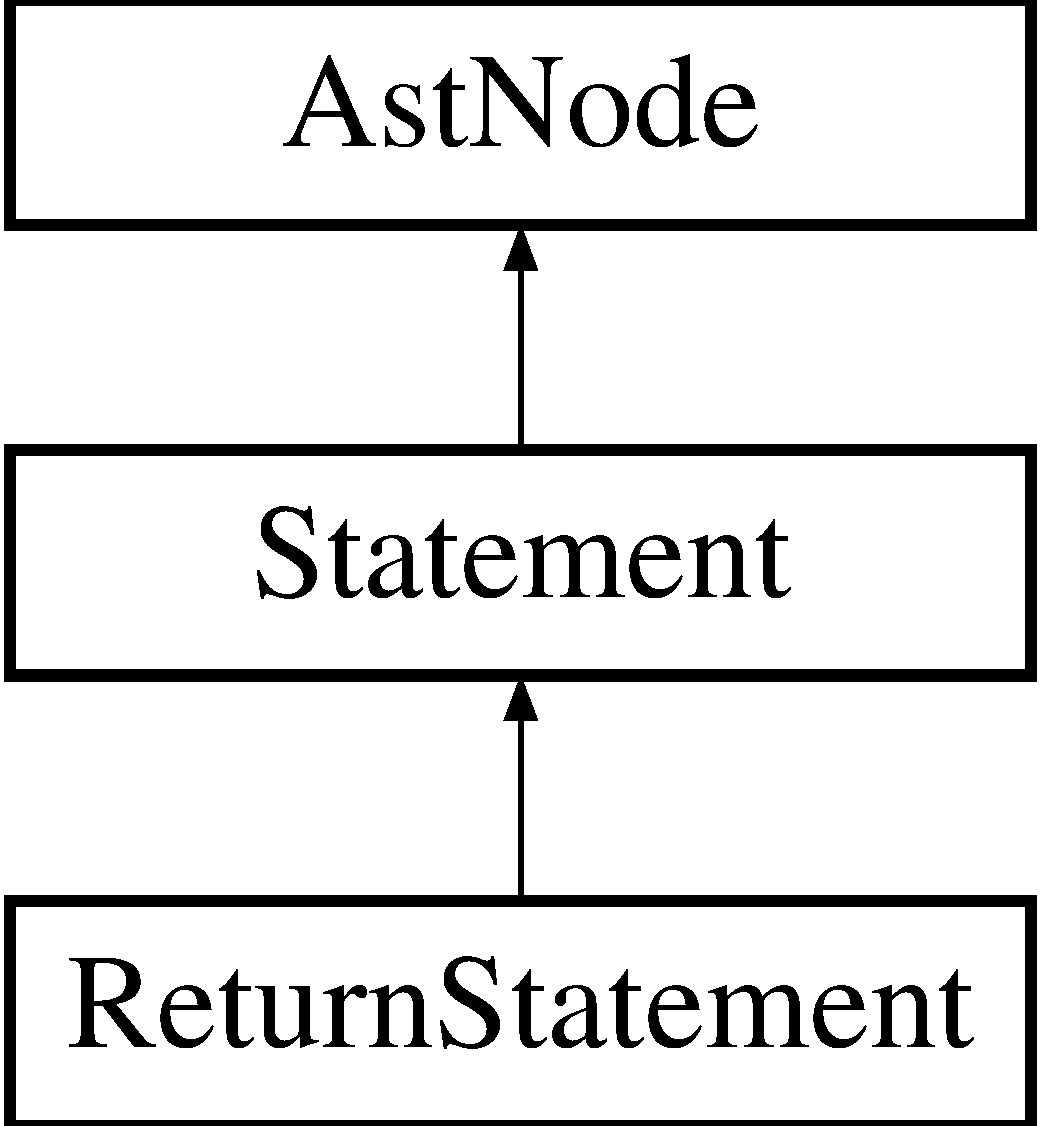
\includegraphics[height=3cm]{classReturnStatement}
\end{center}
\end{figure}
\subsection*{Public Member Functions}
\begin{DoxyCompactItemize}
\item 
\hyperlink{classReturnStatement_a24684312040304edbc031695431317ff}{ReturnStatement} (int lno, ENTRY $\ast$e, \hyperlink{classExpression}{Expression} $\ast$exp)
\item 
ENTRY $\ast$ \hyperlink{classReturnStatement_acecfc9f66e24cc51f1038234cf886229}{getEntry} ()
\item 
void \hyperlink{classReturnStatement_a92ec20af78eb69baae892b95946ceeb5}{setEntry} (ENTRY $\ast$e)
\item 
\hyperlink{classExpression}{Expression} $\ast$ \hyperlink{classReturnStatement_a219347b1f7f79387888f3252a7e07bad}{getExpression} ()
\item 
void \hyperlink{classReturnStatement_a491cb39772b9054be31d27dbc0d72d0f}{accept} (\hyperlink{classAstVisitor}{AstVisitor} $\ast$aVisitor)
\end{DoxyCompactItemize}


\subsection{Detailed Description}
This class represents a TinyJava return statement, with or without an expression. A return statement is represented by:
\begin{DoxyItemize}
\item an \hyperlink{classExpression}{Expression} representing the value to be returned (may be NULL)
\item a pointer to the symbol table ENTRY for the name may also be included (may be initially NULL).
\end{DoxyItemize}

ENTRY should be defined as a macro, and its value should be a class, which is the root of the symbol table entry hierarchy. Its default value is Entry. The macro should be defined at the beginning of the header file Ast.h. 

\subsection{Constructor \& Destructor Documentation}
\hypertarget{classReturnStatement_a24684312040304edbc031695431317ff}{
\index{ReturnStatement@{ReturnStatement}!ReturnStatement@{ReturnStatement}}
\index{ReturnStatement@{ReturnStatement}!ReturnStatement@{ReturnStatement}}
\subsubsection[{ReturnStatement}]{\setlength{\rightskip}{0pt plus 5cm}ReturnStatement::ReturnStatement (int {\em lno}, \/  ENTRY $\ast$ {\em e}, \/  {\bf Expression} $\ast$ {\em exp})\hspace{0.3cm}{\ttfamily  \mbox{[}inline\mbox{]}}}}
\label{classReturnStatement_a24684312040304edbc031695431317ff}
Create a new \hyperlink{classReturnStatement}{ReturnStatement} object.


\begin{DoxyParams}{Parameters}
\item[{\em lno}]is a source line number with the return statement \item[{\em e}]is a pointer to the symbol tabel ENTRY representing the method \item[{\em exp}]is a pointer to an expression node representing the return value expression \end{DoxyParams}

\begin{DoxyExceptions}{Exceptions}
\item[{\em \hyperlink{classAstException}{AstException}}]if the symbol table ENTRY or the expression is NULL \end{DoxyExceptions}


\subsection{Member Function Documentation}
\hypertarget{classReturnStatement_a491cb39772b9054be31d27dbc0d72d0f}{
\index{ReturnStatement@{ReturnStatement}!accept@{accept}}
\index{accept@{accept}!ReturnStatement@{ReturnStatement}}
\subsubsection[{accept}]{\setlength{\rightskip}{0pt plus 5cm}void ReturnStatement::accept ({\bf AstVisitor} $\ast$ {\em aVisitor})\hspace{0.3cm}{\ttfamily  \mbox{[}inline, virtual\mbox{]}}}}
\label{classReturnStatement_a491cb39772b9054be31d27dbc0d72d0f}
Accept a visitor to this node. 
\begin{DoxyParams}{Parameters}
\item[{\em aVisitor}]is a visitor object of type \hyperlink{classAstVisitor}{AstVisitor}. \end{DoxyParams}


Implements \hyperlink{classAstNode_a67b2d6ce1262da2954fb4db255759fb3}{AstNode}.\hypertarget{classReturnStatement_acecfc9f66e24cc51f1038234cf886229}{
\index{ReturnStatement@{ReturnStatement}!getEntry@{getEntry}}
\index{getEntry@{getEntry}!ReturnStatement@{ReturnStatement}}
\subsubsection[{getEntry}]{\setlength{\rightskip}{0pt plus 5cm}ENTRY$\ast$ ReturnStatement::getEntry ()\hspace{0.3cm}{\ttfamily  \mbox{[}inline\mbox{]}}}}
\label{classReturnStatement_acecfc9f66e24cc51f1038234cf886229}
Return the symbol table ENTRY representing the method within which the return statement is included.

\begin{DoxyReturn}{Returns}
ENTRY pointer to the symbol table ENTRY representing the method of the return 
\end{DoxyReturn}
\hypertarget{classReturnStatement_a219347b1f7f79387888f3252a7e07bad}{
\index{ReturnStatement@{ReturnStatement}!getExpression@{getExpression}}
\index{getExpression@{getExpression}!ReturnStatement@{ReturnStatement}}
\subsubsection[{getExpression}]{\setlength{\rightskip}{0pt plus 5cm}{\bf Expression}$\ast$ ReturnStatement::getExpression ()\hspace{0.3cm}{\ttfamily  \mbox{[}inline\mbox{]}}}}
\label{classReturnStatement_a219347b1f7f79387888f3252a7e07bad}
Return the \hyperlink{classExpression}{Expression} pointer representing the return expression.

\begin{DoxyReturn}{Returns}
\hyperlink{classExpression}{Expression} pointer representing the return value expression. 
\end{DoxyReturn}
\hypertarget{classReturnStatement_a92ec20af78eb69baae892b95946ceeb5}{
\index{ReturnStatement@{ReturnStatement}!setEntry@{setEntry}}
\index{setEntry@{setEntry}!ReturnStatement@{ReturnStatement}}
\subsubsection[{setEntry}]{\setlength{\rightskip}{0pt plus 5cm}void ReturnStatement::setEntry (ENTRY $\ast$ {\em e})\hspace{0.3cm}{\ttfamily  \mbox{[}inline\mbox{]}}}}
\label{classReturnStatement_a92ec20af78eb69baae892b95946ceeb5}
Set the symbol table ENTRY representing the method within which the return statement is included.


\begin{DoxyParams}{Parameters}
\item[{\em e}]a pointer to a new symbol table ENTRY representing the method of the return \end{DoxyParams}


The documentation for this class was generated from the following file:\begin{DoxyCompactItemize}
\item 
ReturnStmt.h\end{DoxyCompactItemize}

\hypertarget{classStatement}{
\section{Statement Class Reference}
\label{classStatement}\index{Statement@{Statement}}
}


This class is the parent of all statement Abstract Syntax Tree nodes.  


{\ttfamily \#include $<$Statement.h$>$}Inheritance diagram for Statement::\begin{figure}[H]
\begin{center}
\leavevmode
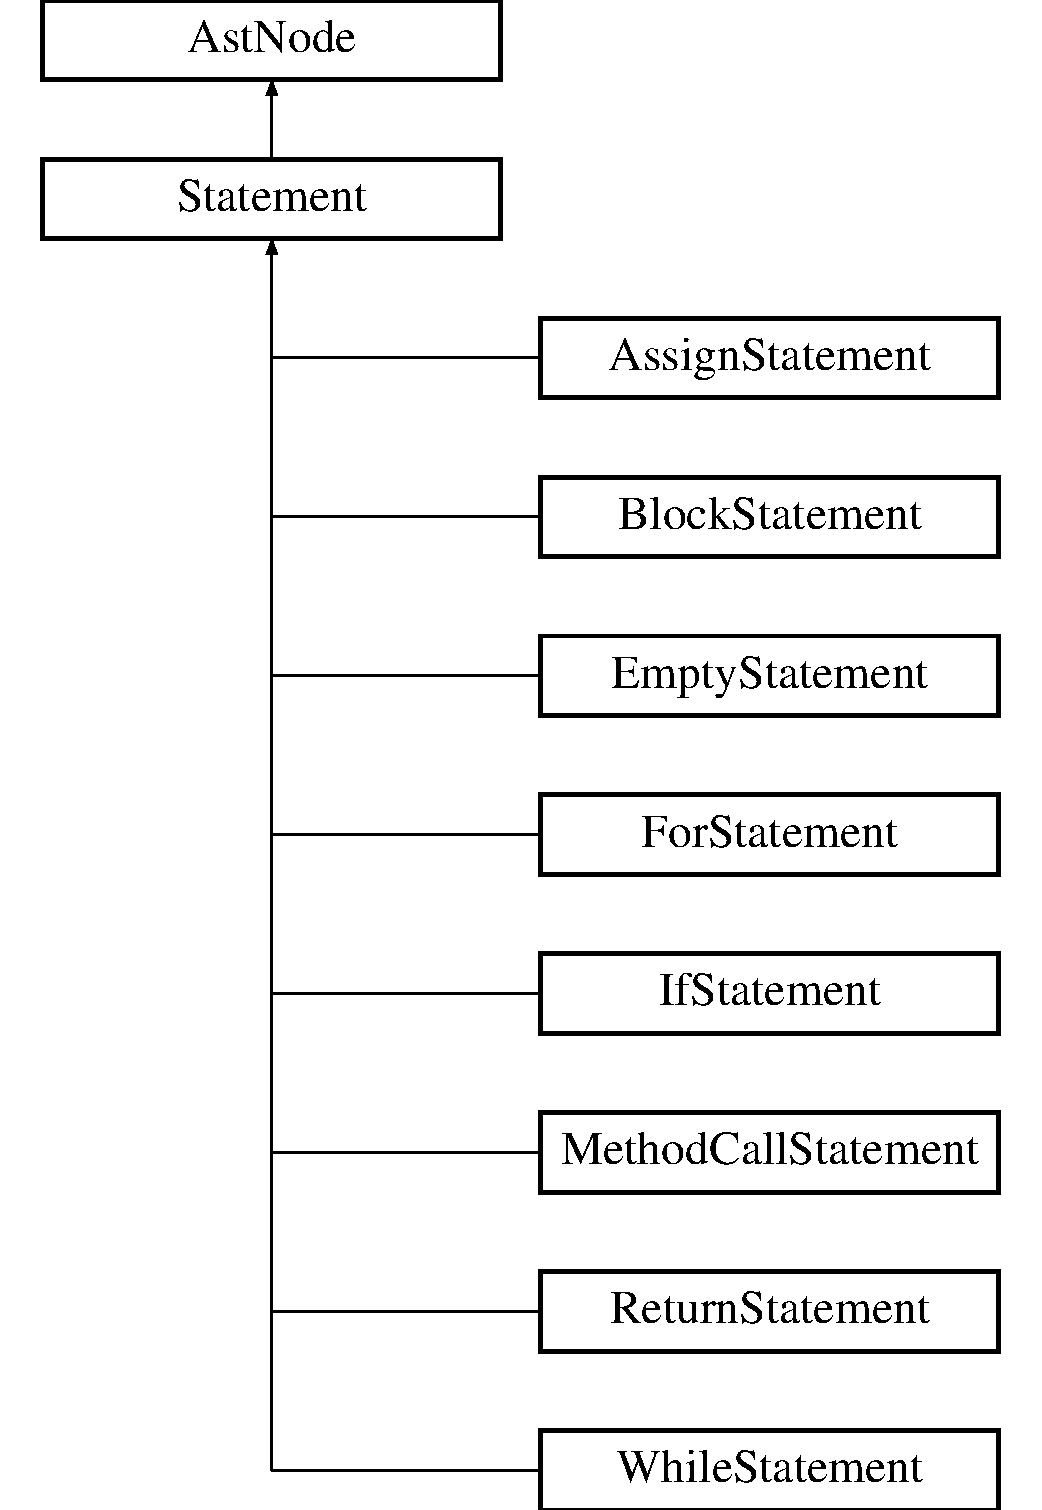
\includegraphics[height=10cm]{classStatement}
\end{center}
\end{figure}


\subsection{Detailed Description}
This class is the parent of all statement Abstract Syntax Tree nodes. This class will not have direct instances. It only serves as the common parent class of:


\begin{DoxyItemize}
\item \hyperlink{classAssignStatement}{AssignStatement}
\item \hyperlink{classBlockStatement}{BlockStatement}
\item \hyperlink{classEmptyStatement}{EmptyStatement}
\item \hyperlink{classForStatement}{ForStatement}
\item \hyperlink{classIfStatement}{IfStatement}
\item \hyperlink{classMethodCallStatement}{MethodCallStatement}
\item \hyperlink{classReturnStatement}{ReturnStatement}
\item \hyperlink{classWhileStatement}{WhileStatement} 
\end{DoxyItemize}

The documentation for this class was generated from the following file:\begin{DoxyCompactItemize}
\item 
Statement.h\end{DoxyCompactItemize}

\hypertarget{classUnaryExpression}{
\section{UnaryExpression Class Reference}
\label{classUnaryExpression}\index{UnaryExpression@{UnaryExpression}}
}


This class represents a TinyJava (prefix or postfix) unary expression involving a unary operator and an operand expression.  


{\ttfamily \#include $<$UnaryExpression.h$>$}Inheritance diagram for UnaryExpression::\begin{figure}[H]
\begin{center}
\leavevmode
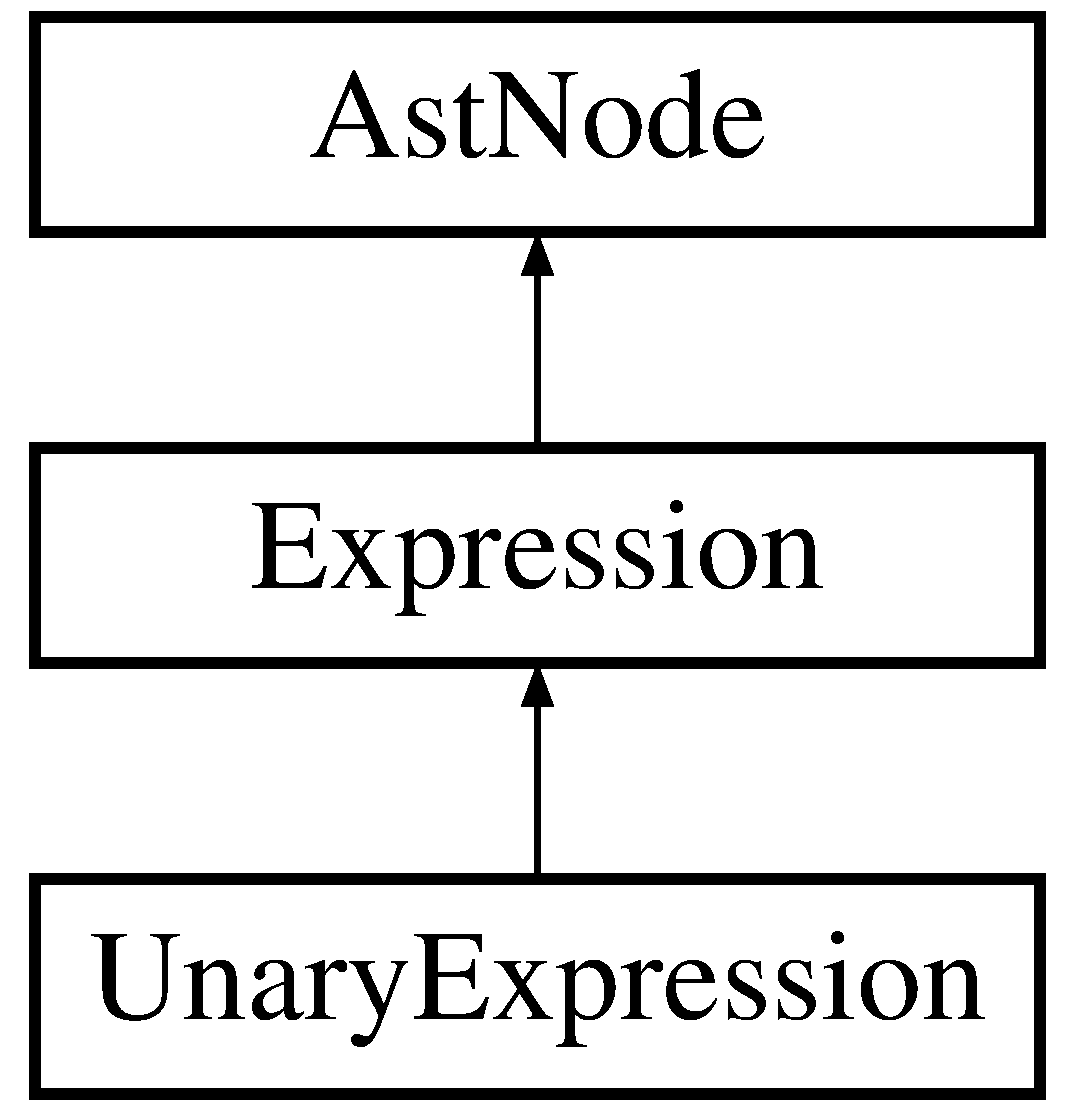
\includegraphics[height=3cm]{classUnaryExpression}
\end{center}
\end{figure}
\subsection*{Public Member Functions}
\begin{DoxyCompactItemize}
\item 
\hyperlink{classUnaryExpression_a03b712bd21c8ec768ae8bdd95ef325f0}{UnaryExpression} (int lno, int op, \hyperlink{classExpression}{Expression} $\ast$arg, bool post=false)
\item 
int \hyperlink{classUnaryExpression_a9818b1b3ddfaa787e321ec28fea399dc}{getOperator} ()
\item 
\hyperlink{classExpression}{Expression} $\ast$ \hyperlink{classUnaryExpression_aca23f932e421218f5e260f09acd99b51}{getOperand} ()
\item 
void \hyperlink{classUnaryExpression_a6c05bb27e3025ec166041091e4023eaf}{setOperand} (\hyperlink{classExpression}{Expression} $\ast$arg)
\item 
bool \hyperlink{classUnaryExpression_aa7905d7a0bd4197cb72af72c8218194c}{isPostfix} ()
\item 
void \hyperlink{classUnaryExpression_a555e53bb0a187856275b8d2c885b75d0}{accept} (\hyperlink{classAstVisitor}{AstVisitor} $\ast$aVisitor)
\end{DoxyCompactItemize}


\subsection{Detailed Description}
This class represents a TinyJava (prefix or postfix) unary expression involving a unary operator and an operand expression. A unary expression is represented by:
\begin{DoxyItemize}
\item an operator (which must be an arithmetic operator)
\item information if it is a postfix unary expression
\item an operand \hyperlink{classExpression}{Expression} subtree representing the operator's argument 
\end{DoxyItemize}

\subsection{Constructor \& Destructor Documentation}
\hypertarget{classUnaryExpression_a03b712bd21c8ec768ae8bdd95ef325f0}{
\index{UnaryExpression@{UnaryExpression}!UnaryExpression@{UnaryExpression}}
\index{UnaryExpression@{UnaryExpression}!UnaryExpression@{UnaryExpression}}
\subsubsection[{UnaryExpression}]{\setlength{\rightskip}{0pt plus 5cm}UnaryExpression::UnaryExpression (int {\em lno}, \/  int {\em op}, \/  {\bf Expression} $\ast$ {\em arg}, \/  bool {\em post} = {\ttfamily false})\hspace{0.3cm}{\ttfamily  \mbox{[}inline\mbox{]}}}}
\label{classUnaryExpression_a03b712bd21c8ec768ae8bdd95ef325f0}
Create a new \hyperlink{classUnaryExpression}{UnaryExpression} object.


\begin{DoxyParams}{Parameters}
\item[{\em lno}]source code line number with the unary expression. \item[{\em op}]an int value representing the operator; it should be one of the constants defined in the \hyperlink{classAstNode}{AstNode} class \item[{\em arg}]an \hyperlink{classExpression}{Expression} representing the operand \item[{\em post}]a boolean value indicating if it is a postfix unary expression; the default is false \end{DoxyParams}

\begin{DoxyExceptions}{Exceptions}
\item[{\em \hyperlink{classAstException}{AstException}}]if either the arg operand is NULL \end{DoxyExceptions}


\subsection{Member Function Documentation}
\hypertarget{classUnaryExpression_a555e53bb0a187856275b8d2c885b75d0}{
\index{UnaryExpression@{UnaryExpression}!accept@{accept}}
\index{accept@{accept}!UnaryExpression@{UnaryExpression}}
\subsubsection[{accept}]{\setlength{\rightskip}{0pt plus 5cm}void UnaryExpression::accept ({\bf AstVisitor} $\ast$ {\em aVisitor})\hspace{0.3cm}{\ttfamily  \mbox{[}inline, virtual\mbox{]}}}}
\label{classUnaryExpression_a555e53bb0a187856275b8d2c885b75d0}
Accept a visitor to this node. 
\begin{DoxyParams}{Parameters}
\item[{\em aVisitor}]is a visitor object of type \hyperlink{classAstVisitor}{AstVisitor}. \end{DoxyParams}


Implements \hyperlink{classAstNode_a67b2d6ce1262da2954fb4db255759fb3}{AstNode}.\hypertarget{classUnaryExpression_aca23f932e421218f5e260f09acd99b51}{
\index{UnaryExpression@{UnaryExpression}!getOperand@{getOperand}}
\index{getOperand@{getOperand}!UnaryExpression@{UnaryExpression}}
\subsubsection[{getOperand}]{\setlength{\rightskip}{0pt plus 5cm}{\bf Expression}$\ast$ UnaryExpression::getOperand ()\hspace{0.3cm}{\ttfamily  \mbox{[}inline\mbox{]}}}}
\label{classUnaryExpression_aca23f932e421218f5e260f09acd99b51}
Return the operand of this unary expression.

\begin{DoxyReturn}{Returns}
the \hyperlink{classExpression}{Expression} pointer which is the operand expression tree 
\end{DoxyReturn}
\hypertarget{classUnaryExpression_a9818b1b3ddfaa787e321ec28fea399dc}{
\index{UnaryExpression@{UnaryExpression}!getOperator@{getOperator}}
\index{getOperator@{getOperator}!UnaryExpression@{UnaryExpression}}
\subsubsection[{getOperator}]{\setlength{\rightskip}{0pt plus 5cm}int UnaryExpression::getOperator ()\hspace{0.3cm}{\ttfamily  \mbox{[}inline\mbox{]}}}}
\label{classUnaryExpression_a9818b1b3ddfaa787e321ec28fea399dc}
Return the operator of this unary expression.

\begin{DoxyReturn}{Returns}
operator, as defined in the \hyperlink{classAstNode}{AstNode} class. 
\end{DoxyReturn}
\hypertarget{classUnaryExpression_aa7905d7a0bd4197cb72af72c8218194c}{
\index{UnaryExpression@{UnaryExpression}!isPostfix@{isPostfix}}
\index{isPostfix@{isPostfix}!UnaryExpression@{UnaryExpression}}
\subsubsection[{isPostfix}]{\setlength{\rightskip}{0pt plus 5cm}bool UnaryExpression::isPostfix ()\hspace{0.3cm}{\ttfamily  \mbox{[}inline\mbox{]}}}}
\label{classUnaryExpression_aa7905d7a0bd4197cb72af72c8218194c}
Is it a postfix unary expression?

\begin{DoxyReturn}{Returns}
a boolean value indicating if it is a postifx unary expression 
\end{DoxyReturn}
\hypertarget{classUnaryExpression_a6c05bb27e3025ec166041091e4023eaf}{
\index{UnaryExpression@{UnaryExpression}!setOperand@{setOperand}}
\index{setOperand@{setOperand}!UnaryExpression@{UnaryExpression}}
\subsubsection[{setOperand}]{\setlength{\rightskip}{0pt plus 5cm}void UnaryExpression::setOperand ({\bf Expression} $\ast$ {\em arg})\hspace{0.3cm}{\ttfamily  \mbox{[}inline\mbox{]}}}}
\label{classUnaryExpression_a6c05bb27e3025ec166041091e4023eaf}
Set the operand expression of this unary expression.


\begin{DoxyParams}{Parameters}
\item[{\em arg}]the expression to be the new operand \end{DoxyParams}

\begin{DoxyExceptions}{Exceptions}
\item[{\em \hyperlink{classAstException}{AstException}}]if the argument expression is NULL \end{DoxyExceptions}


The documentation for this class was generated from the following file:\begin{DoxyCompactItemize}
\item 
UnaryExpression.h\end{DoxyCompactItemize}

\hypertarget{classVariableDeclaration}{
\section{VariableDeclaration Class Reference}
\label{classVariableDeclaration}\index{VariableDeclaration@{VariableDeclaration}}
}


This class represents a declaration of a local variable in a TinyJava class method.  


{\ttfamily \#include $<$VariableDeclaration.h$>$}Inheritance diagram for VariableDeclaration::\begin{figure}[H]
\begin{center}
\leavevmode
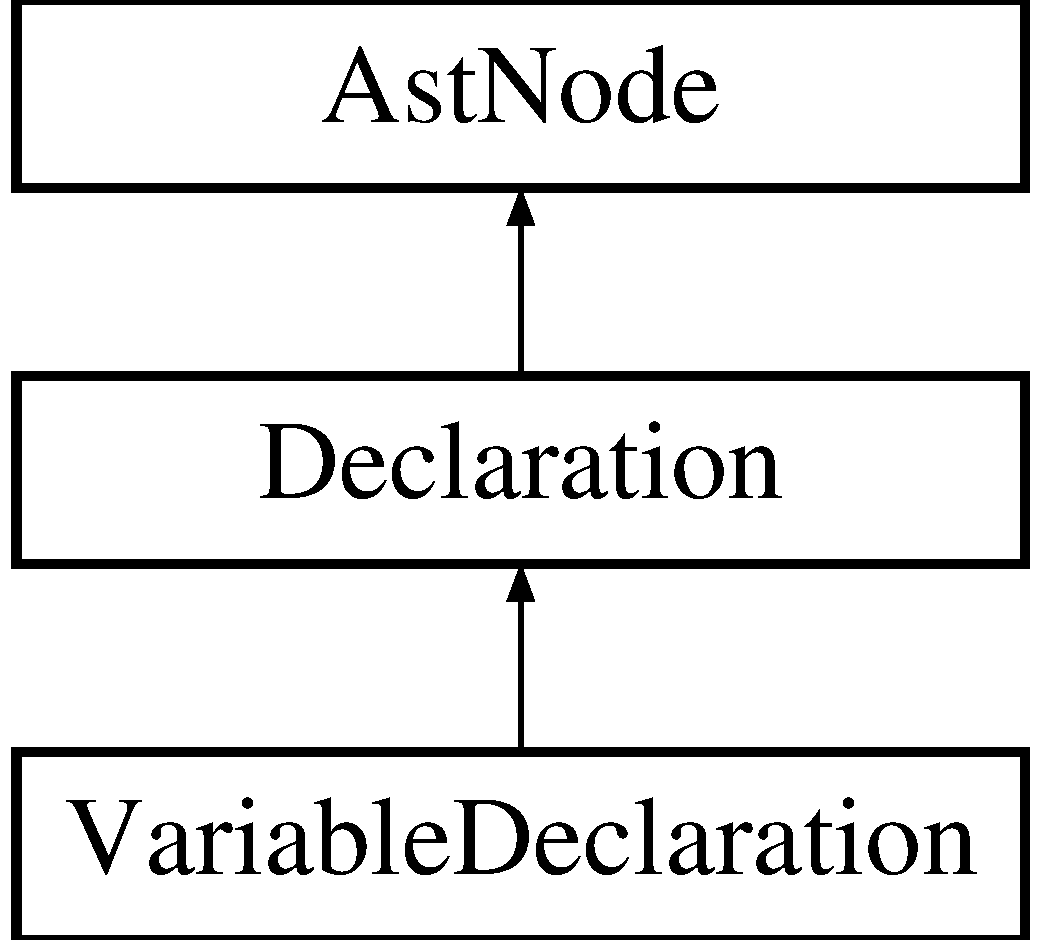
\includegraphics[height=3cm]{classVariableDeclaration}
\end{center}
\end{figure}
\subsection*{Public Member Functions}
\begin{DoxyCompactItemize}
\item 
\hyperlink{classVariableDeclaration_a4d671e248b007508b41e69a6c0571957}{VariableDeclaration} (int lno, const char $\ast$nm, int tp, const char $\ast$iv)
\item 
const char $\ast$ \hyperlink{classVariableDeclaration_a0651102c92331f832679816bccd08ddd}{getName} ()
\item 
void \hyperlink{classVariableDeclaration_a87d34512598049ef3f1d945451873ab5}{setName} (const char $\ast$nm)
\item 
int \hyperlink{classVariableDeclaration_a1384f2df0a1fcc9d2f55a20d4db0d34b}{getType} ()
\item 
void \hyperlink{classVariableDeclaration_a3fbc1e04d3d8e6aa487ced5215347b51}{setType} (int tp)
\item 
const char $\ast$ \hyperlink{classVariableDeclaration_ad4e01c324003e1730afcfe3a231ee2a0}{getInitValue} ()
\item 
void \hyperlink{classVariableDeclaration_a4bdb316526fd2c35221c6b65aa667bc7}{setInitValue} (const char $\ast$iv)
\item 
ENTRY $\ast$ \hyperlink{classVariableDeclaration_a42520812cc7fd155b4d30852ca1c68f7}{getEntry} ()
\item 
void \hyperlink{classVariableDeclaration_a42cfc2417b553b93190b937d7413a32c}{setEntry} (ENTRY $\ast$e)
\item 
void \hyperlink{classVariableDeclaration_af8e0086b00a9bc45f2aff7bf91d8f17d}{accept} (\hyperlink{classAstVisitor}{AstVisitor} $\ast$aVisitor)
\end{DoxyCompactItemize}


\subsection{Detailed Description}
This class represents a declaration of a local variable in a TinyJava class method. A variable is represented by:
\begin{DoxyItemize}
\item variable name -\/ a string
\item type -\/ an integer value, as defined in the \hyperlink{classAstNode}{AstNode} class
\item initial value -\/ a string representing the initial value (a literal)
\item a pointer to the symbol table ENTRY for the variable (which may be initially undefined).
\end{DoxyItemize}

ENTRY should be defined as a macro, and its value should be a class, which is the root of the symbol table entry hierarchy. Its default value is Entry. The macro should be defined at the beginning of the header file Ast.h. 

\subsection{Constructor \& Destructor Documentation}
\hypertarget{classVariableDeclaration_a4d671e248b007508b41e69a6c0571957}{
\index{VariableDeclaration@{VariableDeclaration}!VariableDeclaration@{VariableDeclaration}}
\index{VariableDeclaration@{VariableDeclaration}!VariableDeclaration@{VariableDeclaration}}
\subsubsection[{VariableDeclaration}]{\setlength{\rightskip}{0pt plus 5cm}VariableDeclaration::VariableDeclaration (int {\em lno}, \/  const char $\ast$ {\em nm}, \/  int {\em tp}, \/  const char $\ast$ {\em iv})\hspace{0.3cm}{\ttfamily  \mbox{[}inline\mbox{]}}}}
\label{classVariableDeclaration_a4d671e248b007508b41e69a6c0571957}
Create a new \hyperlink{classVariableDeclaration}{VariableDeclaration} object.


\begin{DoxyParams}{Parameters}
\item[{\em lno}]a source code line number with the variable declaration. \item[{\em nm}]a string with the variable name \item[{\em tp}]an integer representing the type, as defined in the \hyperlink{classAstNode}{AstNode} class \item[{\em iv}]a string with the initial value (a literal) \end{DoxyParams}

\begin{DoxyExceptions}{Exceptions}
\item[{\em \hyperlink{classAstException}{AstException}}]if the variable name or the initial value is NULL \end{DoxyExceptions}


\subsection{Member Function Documentation}
\hypertarget{classVariableDeclaration_af8e0086b00a9bc45f2aff7bf91d8f17d}{
\index{VariableDeclaration@{VariableDeclaration}!accept@{accept}}
\index{accept@{accept}!VariableDeclaration@{VariableDeclaration}}
\subsubsection[{accept}]{\setlength{\rightskip}{0pt plus 5cm}void VariableDeclaration::accept ({\bf AstVisitor} $\ast$ {\em aVisitor})\hspace{0.3cm}{\ttfamily  \mbox{[}inline, virtual\mbox{]}}}}
\label{classVariableDeclaration_af8e0086b00a9bc45f2aff7bf91d8f17d}
Accept a visitor to this node. 
\begin{DoxyParams}{Parameters}
\item[{\em aVisitor}]is a visitor object of type \hyperlink{classAstVisitor}{AstVisitor}. \end{DoxyParams}


Implements \hyperlink{classAstNode_a67b2d6ce1262da2954fb4db255759fb3}{AstNode}.\hypertarget{classVariableDeclaration_a42520812cc7fd155b4d30852ca1c68f7}{
\index{VariableDeclaration@{VariableDeclaration}!getEntry@{getEntry}}
\index{getEntry@{getEntry}!VariableDeclaration@{VariableDeclaration}}
\subsubsection[{getEntry}]{\setlength{\rightskip}{0pt plus 5cm}ENTRY$\ast$ VariableDeclaration::getEntry ()\hspace{0.3cm}{\ttfamily  \mbox{[}inline\mbox{]}}}}
\label{classVariableDeclaration_a42520812cc7fd155b4d30852ca1c68f7}
Return a pointer to the symbol table ENTRY representing this variable This value may be undefined before the symbol table is created.

\begin{DoxyReturn}{Returns}
a pointer to the symbol table ENTRY representing this variable 
\end{DoxyReturn}
\hypertarget{classVariableDeclaration_ad4e01c324003e1730afcfe3a231ee2a0}{
\index{VariableDeclaration@{VariableDeclaration}!getInitValue@{getInitValue}}
\index{getInitValue@{getInitValue}!VariableDeclaration@{VariableDeclaration}}
\subsubsection[{getInitValue}]{\setlength{\rightskip}{0pt plus 5cm}const char$\ast$ VariableDeclaration::getInitValue ()\hspace{0.3cm}{\ttfamily  \mbox{[}inline\mbox{]}}}}
\label{classVariableDeclaration_ad4e01c324003e1730afcfe3a231ee2a0}
Return the initial value of this \hyperlink{classVariableDeclaration}{VariableDeclaration}.

\begin{DoxyReturn}{Returns}
a string representing the initial value of the variable. 
\end{DoxyReturn}
\hypertarget{classVariableDeclaration_a0651102c92331f832679816bccd08ddd}{
\index{VariableDeclaration@{VariableDeclaration}!getName@{getName}}
\index{getName@{getName}!VariableDeclaration@{VariableDeclaration}}
\subsubsection[{getName}]{\setlength{\rightskip}{0pt plus 5cm}const char$\ast$ VariableDeclaration::getName ()\hspace{0.3cm}{\ttfamily  \mbox{[}inline\mbox{]}}}}
\label{classVariableDeclaration_a0651102c92331f832679816bccd08ddd}
Return the variable name.

\begin{DoxyReturn}{Returns}
string representing the variable name. 
\end{DoxyReturn}
\hypertarget{classVariableDeclaration_a1384f2df0a1fcc9d2f55a20d4db0d34b}{
\index{VariableDeclaration@{VariableDeclaration}!getType@{getType}}
\index{getType@{getType}!VariableDeclaration@{VariableDeclaration}}
\subsubsection[{getType}]{\setlength{\rightskip}{0pt plus 5cm}int VariableDeclaration::getType ()\hspace{0.3cm}{\ttfamily  \mbox{[}inline\mbox{]}}}}
\label{classVariableDeclaration_a1384f2df0a1fcc9d2f55a20d4db0d34b}
Return the type of this \hyperlink{classVariableDeclaration}{VariableDeclaration}.

\begin{DoxyReturn}{Returns}
an integer value representing the type, as defined in the \hyperlink{classAstNode}{AstNode} class. 
\end{DoxyReturn}
\hypertarget{classVariableDeclaration_a42cfc2417b553b93190b937d7413a32c}{
\index{VariableDeclaration@{VariableDeclaration}!setEntry@{setEntry}}
\index{setEntry@{setEntry}!VariableDeclaration@{VariableDeclaration}}
\subsubsection[{setEntry}]{\setlength{\rightskip}{0pt plus 5cm}void VariableDeclaration::setEntry (ENTRY $\ast$ {\em e})\hspace{0.3cm}{\ttfamily  \mbox{[}inline\mbox{]}}}}
\label{classVariableDeclaration_a42cfc2417b553b93190b937d7413a32c}
Set the pointer to the symbol table ENTRY representing this variable. This value will typically be set during the symbol table construction phase.


\begin{DoxyParams}{Parameters}
\item[{\em e}]the pointer to the symbol table ENTRY representing this variable \end{DoxyParams}
\hypertarget{classVariableDeclaration_a4bdb316526fd2c35221c6b65aa667bc7}{
\index{VariableDeclaration@{VariableDeclaration}!setInitValue@{setInitValue}}
\index{setInitValue@{setInitValue}!VariableDeclaration@{VariableDeclaration}}
\subsubsection[{setInitValue}]{\setlength{\rightskip}{0pt plus 5cm}void VariableDeclaration::setInitValue (const char $\ast$ {\em iv})\hspace{0.3cm}{\ttfamily  \mbox{[}inline\mbox{]}}}}
\label{classVariableDeclaration_a4bdb316526fd2c35221c6b65aa667bc7}
Set the new initial value of this \hyperlink{classVariableDeclaration}{VariableDeclaration}.


\begin{DoxyParams}{Parameters}
\item[{\em iv}]a string representing the initial value of this variable \end{DoxyParams}

\begin{DoxyExceptions}{Exceptions}
\item[{\em \hyperlink{classAstException}{AstException}}]if the initial value is NULL \end{DoxyExceptions}
\hypertarget{classVariableDeclaration_a87d34512598049ef3f1d945451873ab5}{
\index{VariableDeclaration@{VariableDeclaration}!setName@{setName}}
\index{setName@{setName}!VariableDeclaration@{VariableDeclaration}}
\subsubsection[{setName}]{\setlength{\rightskip}{0pt plus 5cm}void VariableDeclaration::setName (const char $\ast$ {\em nm})\hspace{0.3cm}{\ttfamily  \mbox{[}inline\mbox{]}}}}
\label{classVariableDeclaration_a87d34512598049ef3f1d945451873ab5}
Set the variable name.


\begin{DoxyParams}{Parameters}
\item[{\em nm}]a string representing the new name of the variable. \end{DoxyParams}
\hypertarget{classVariableDeclaration_a3fbc1e04d3d8e6aa487ced5215347b51}{
\index{VariableDeclaration@{VariableDeclaration}!setType@{setType}}
\index{setType@{setType}!VariableDeclaration@{VariableDeclaration}}
\subsubsection[{setType}]{\setlength{\rightskip}{0pt plus 5cm}void VariableDeclaration::setType (int {\em tp})\hspace{0.3cm}{\ttfamily  \mbox{[}inline\mbox{]}}}}
\label{classVariableDeclaration_a3fbc1e04d3d8e6aa487ced5215347b51}
Set the new type of this \hyperlink{classVariableDeclaration}{VariableDeclaration}.


\begin{DoxyParams}{Parameters}
\item[{\em tp}]an integer value representing the type, as defined in the \hyperlink{classAstNode}{AstNode} class. \end{DoxyParams}


The documentation for this class was generated from the following file:\begin{DoxyCompactItemize}
\item 
VariableDeclaration.h\end{DoxyCompactItemize}

\hypertarget{classWhileStatement}{
\section{WhileStatement Class Reference}
\label{classWhileStatement}\index{WhileStatement@{WhileStatement}}
}


This class represents a TinyJava WHILE statement.  


{\ttfamily \#include $<$WhileStmt.h$>$}Inheritance diagram for WhileStatement::\begin{figure}[H]
\begin{center}
\leavevmode
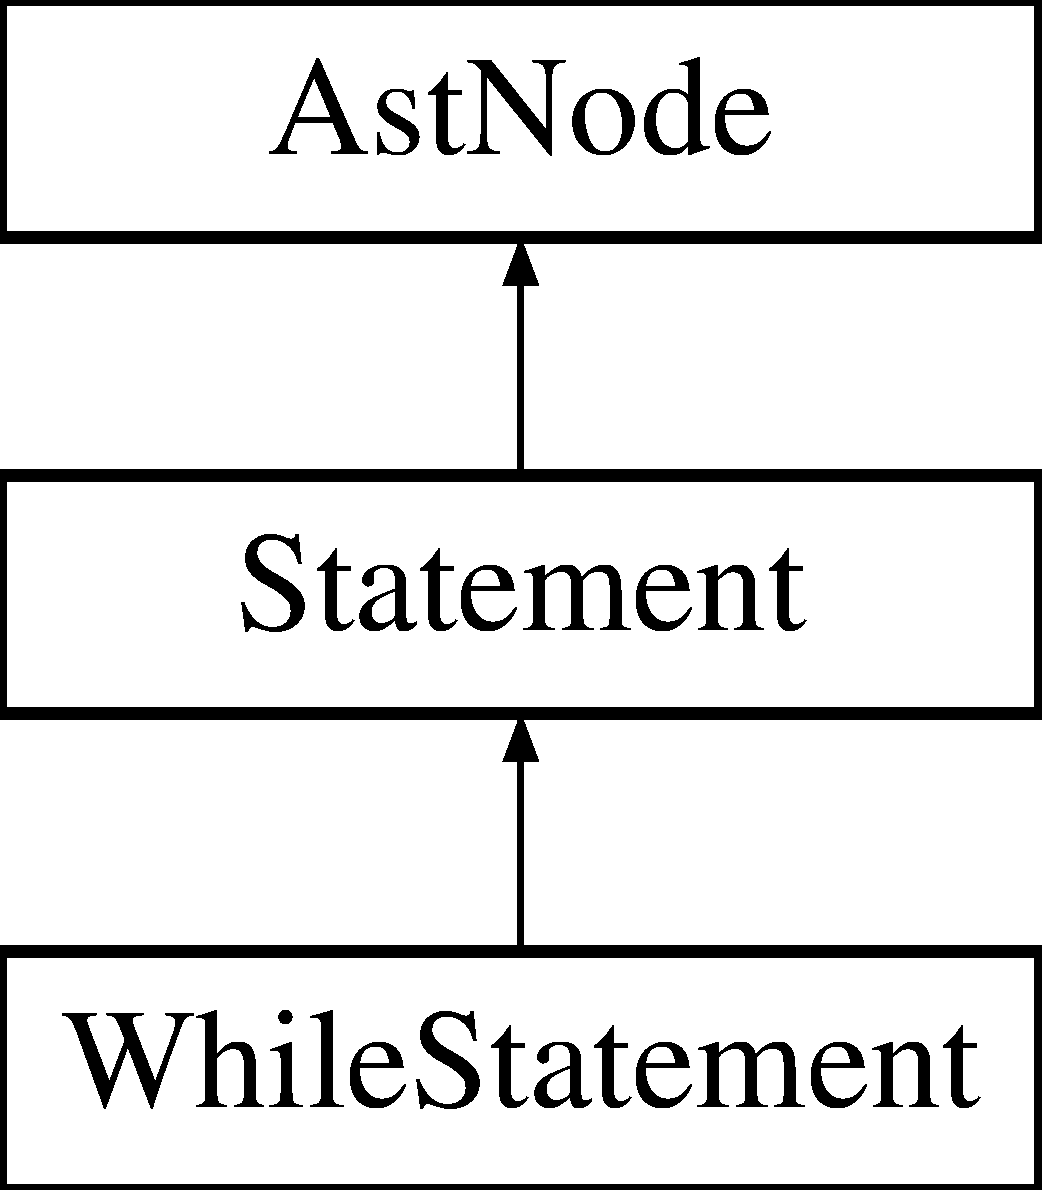
\includegraphics[height=3cm]{classWhileStatement}
\end{center}
\end{figure}
\subsection*{Public Member Functions}
\begin{DoxyCompactItemize}
\item 
\hyperlink{classWhileStatement_ab75b71383a4c7f1c8ad103cab6f02b10}{WhileStatement} (int lno, \hyperlink{classExpression}{Expression} $\ast$e, \hyperlink{classStatement}{Statement} $\ast$b)
\item 
\hyperlink{classExpression}{Expression} $\ast$ \hyperlink{classWhileStatement_a8ccd99538f16bc15feb7f7eff947a923}{getExpression} ()
\item 
\hyperlink{classStatement}{Statement} $\ast$ \hyperlink{classWhileStatement_a68631c014236d2a635aa4395c6dd229c}{getBodyStatement} ()
\item 
void \hyperlink{classWhileStatement_abde6377670b22bad622f1a2ec2aade65}{setBodyStatement} (\hyperlink{classStatement}{Statement} $\ast$b)
\item 
void \hyperlink{classWhileStatement_aeb7e6e61053a3e8a7b82a54c4eb8bf0d}{accept} (\hyperlink{classAstVisitor}{AstVisitor} $\ast$aVisitor)
\end{DoxyCompactItemize}


\subsection{Detailed Description}
This class represents a TinyJava WHILE statement. A while statement is represented by:
\begin{DoxyItemize}
\item a control \hyperlink{classExpression}{Expression} representation
\item the while loop body \hyperlink{classStatement}{Statement} representation 
\end{DoxyItemize}

\subsection{Constructor \& Destructor Documentation}
\hypertarget{classWhileStatement_ab75b71383a4c7f1c8ad103cab6f02b10}{
\index{WhileStatement@{WhileStatement}!WhileStatement@{WhileStatement}}
\index{WhileStatement@{WhileStatement}!WhileStatement@{WhileStatement}}
\subsubsection[{WhileStatement}]{\setlength{\rightskip}{0pt plus 5cm}WhileStatement::WhileStatement (int {\em lno}, \/  {\bf Expression} $\ast$ {\em e}, \/  {\bf Statement} $\ast$ {\em b})\hspace{0.3cm}{\ttfamily  \mbox{[}inline\mbox{]}}}}
\label{classWhileStatement_ab75b71383a4c7f1c8ad103cab6f02b10}
Create a new \hyperlink{classWhileStatement}{WhileStatement} object


\begin{DoxyParams}{Parameters}
\item[{\em lno}]a source code line number with the while statement (should be the beginning of the while statement) \item[{\em e}]a pointer to the control \hyperlink{classExpression}{Expression} syntax tree \item[{\em b}]a pointer to the \hyperlink{classStatement}{Statement} body syntax tree \end{DoxyParams}

\begin{DoxyExceptions}{Exceptions}
\item[{\em \hyperlink{classAstException}{AstException}}]if either the e or b argument is NULL \end{DoxyExceptions}


\subsection{Member Function Documentation}
\hypertarget{classWhileStatement_aeb7e6e61053a3e8a7b82a54c4eb8bf0d}{
\index{WhileStatement@{WhileStatement}!accept@{accept}}
\index{accept@{accept}!WhileStatement@{WhileStatement}}
\subsubsection[{accept}]{\setlength{\rightskip}{0pt plus 5cm}void WhileStatement::accept ({\bf AstVisitor} $\ast$ {\em aVisitor})\hspace{0.3cm}{\ttfamily  \mbox{[}inline, virtual\mbox{]}}}}
\label{classWhileStatement_aeb7e6e61053a3e8a7b82a54c4eb8bf0d}
Accept a visitor to this node. 
\begin{DoxyParams}{Parameters}
\item[{\em aVisitor}]is a visitor object of type \hyperlink{classAstVisitor}{AstVisitor}. \end{DoxyParams}


Implements \hyperlink{classAstNode_a67b2d6ce1262da2954fb4db255759fb3}{AstNode}.\hypertarget{classWhileStatement_a68631c014236d2a635aa4395c6dd229c}{
\index{WhileStatement@{WhileStatement}!getBodyStatement@{getBodyStatement}}
\index{getBodyStatement@{getBodyStatement}!WhileStatement@{WhileStatement}}
\subsubsection[{getBodyStatement}]{\setlength{\rightskip}{0pt plus 5cm}{\bf Statement}$\ast$ WhileStatement::getBodyStatement ()\hspace{0.3cm}{\ttfamily  \mbox{[}inline\mbox{]}}}}
\label{classWhileStatement_a68631c014236d2a635aa4395c6dd229c}
Return the body of this while statement

\begin{DoxyReturn}{Returns}
pointer to a \hyperlink{classStatement}{Statement} representing the body of the while statement 
\end{DoxyReturn}
\hypertarget{classWhileStatement_a8ccd99538f16bc15feb7f7eff947a923}{
\index{WhileStatement@{WhileStatement}!getExpression@{getExpression}}
\index{getExpression@{getExpression}!WhileStatement@{WhileStatement}}
\subsubsection[{getExpression}]{\setlength{\rightskip}{0pt plus 5cm}{\bf Expression}$\ast$ WhileStatement::getExpression ()\hspace{0.3cm}{\ttfamily  \mbox{[}inline\mbox{]}}}}
\label{classWhileStatement_a8ccd99538f16bc15feb7f7eff947a923}
Return the control \hyperlink{classExpression}{Expression} of this while statement

\begin{DoxyReturn}{Returns}
pointer to an \hyperlink{classExpression}{Expression} representing the control expression 
\end{DoxyReturn}
\hypertarget{classWhileStatement_abde6377670b22bad622f1a2ec2aade65}{
\index{WhileStatement@{WhileStatement}!setBodyStatement@{setBodyStatement}}
\index{setBodyStatement@{setBodyStatement}!WhileStatement@{WhileStatement}}
\subsubsection[{setBodyStatement}]{\setlength{\rightskip}{0pt plus 5cm}void WhileStatement::setBodyStatement ({\bf Statement} $\ast$ {\em b})\hspace{0.3cm}{\ttfamily  \mbox{[}inline\mbox{]}}}}
\label{classWhileStatement_abde6377670b22bad622f1a2ec2aade65}
Set the the body of this while statement


\begin{DoxyParams}{Parameters}
\item[{\em b}]a pointer to a \hyperlink{classStatement}{Statement} representing the body of the while statement \end{DoxyParams}

\begin{DoxyExceptions}{Exceptions}
\item[{\em \hyperlink{classAstException}{AstException}}]if the argument is NULL \end{DoxyExceptions}


The documentation for this class was generated from the following file:\begin{DoxyCompactItemize}
\item 
WhileStmt.h\end{DoxyCompactItemize}

\printindex
\end{document}
